\documentclass[conference,a4paper]{IEEEtran}
% IEEE conference format (two columns, 10 pt Times, A4), laid out like the reference paper
% "Deep Learning Model for Sign Language Detection with Integrated Morse Code Conversion".
% The publisher's running header/footer (proceedings title, ISBN, DOI, copyright line) is added
% by the conference at publication time and is intentionally not reproduced here.

\usepackage{cite}
\usepackage{amsmath}
\usepackage{graphicx}
\usepackage{array}
\usepackage{booktabs}
\usepackage{multirow}
\usepackage{adjustbox}
\usepackage{textcomp}
\usepackage{xcolor}
\usepackage{tikz}
\usetikzlibrary{positioning,arrows.meta,shapes.geometric,fit,calc}
\usepackage[T1]{fontenc}
\usepackage{url}
\def\BibTeX{{\rm B\kern-.05em{\sc i\kern-.025em b}\kern-.08em
    T\kern-.1667em\lower.7ex\hbox{E}\kern-.125em X}}

\renewcommand{\IEEEkeywordsname}{Keywords}
\setlength{\tabcolsep}{3.5pt}
% columns end where the text ends: with many floats, flush-bottom pages stretch the space between paragraphs
\raggedbottom

% generated by eval/make_paper_assets.js -- do not edit
\newcommand{\nBenchTotal}{24{,}248}
\newcommand{\nBenchFaults}{13{,}356}
\newcommand{\nBenchClean}{10{,}892}
\newcommand{\nBenchClasses}{20}
\newcommand{\nBenchGold}{864}
\newcommand{\nBenchWorkbooks}{72}
\newcommand{\eonevonerejectR}{44.2}
\newcommand{\eonevonerejectF}{61.3}
\newcommand{\eonevonerejectFPR}{0.0}
\newcommand{\eonevonerejectP}{100.0}
\newcommand{\eonevoneflagR}{69.2}
\newcommand{\eonevoneflagF}{76.4}
\newcommand{\eonevoneflagFPR}{14.7}
\newcommand{\eonevoneflagP}{85.2}
\newcommand{\eonevtworejectR}{83.0}
\newcommand{\eonevtworejectF}{90.7}
\newcommand{\eonevtworejectFPR}{0.0}
\newcommand{\eonevtworejectP}{100.0}
\newcommand{\eonevtwoflagR}{92.4}
\newcommand{\eonevtwoflagF}{95.5}
\newcommand{\eonevtwoflagFPR}{1.3}
\newcommand{\eonevtwoflagP}{98.8}
\newcommand{\eonelintrejectR}{27.2}
\newcommand{\eonelintrejectF}{42.4}
\newcommand{\eonelintrejectFPR}{1.3}
\newcommand{\eonelintrejectP}{96.2}
\newcommand{\eonelintflagR}{27.2}
\newcommand{\eonelintflagF}{42.4}
\newcommand{\eonelintflagFPR}{1.3}
\newcommand{\eonelintflagP}{96.2}
\newcommand{\eonesyntaxrejectR}{17.6}
\newcommand{\eonesyntaxrejectF}{29.9}
\newcommand{\eonesyntaxrejectFPR}{0.0}
\newcommand{\eonesyntaxrejectP}{100.0}
\newcommand{\eonesyntaxflagR}{17.6}
\newcommand{\eonesyntaxflagF}{29.9}
\newcommand{\eonesyntaxflagFPR}{0.0}
\newcommand{\eonesyntaxflagP}{100.0}
\newcommand{\ablstructuralRejectR}{62.4}
\newcommand{\ablstructuralRejectF}{76.9}
\newcommand{\ablsymbolsRejectR}{66.5}
\newcommand{\ablsymbolsRejectF}{79.9}
\newcommand{\ablboundsRejectR}{78.5}
\newcommand{\ablboundsRejectF}{87.9}
\newcommand{\ablshapeRejectR}{79.2}
\newcommand{\ablshapeRejectF}{88.4}
\newcommand{\ablgroundingRejectR}{83.0}
\newcommand{\ablgroundingRejectF}{90.7}
\newcommand{\ablcircularRejectR}{50.6}
\newcommand{\ablcircularRejectF}{67.2}
\newcommand{\ablqueryRejectR}{81.9}
\newcommand{\ablqueryRejectF}{90.1}
\newcommand{\visloudN}{10{,}004}
\newcommand{\visloudvoneReject}{46.4}
\newcommand{\visloudvoneFlag}{71.4}
\newcommand{\visloudvtwoReject}{93.7}
\newcommand{\visloudvtwoFlag}{99.7}
\newcommand{\vissilentN}{3{,}352}
\newcommand{\vissilentvoneReject}{37.7}
\newcommand{\vissilentvoneFlag}{62.5}
\newcommand{\vissilentvtwoReject}{50.9}
\newcommand{\vissilentvtwoFlag}{70.7}
\newcommand{\clsrangecontainsselfvoneReject}{0}
\newcommand{\clsrangecontainsselfvoneFlag}{100}
\newcommand{\clsrangecontainsselfvtwoReject}{100}
\newcommand{\clsrangecontainsselfvtwoFlag}{100}
\newcommand{\clsrangecontainsselfN}{864}
\newcommand{\clscolumncontainsselfvoneReject}{0}
\newcommand{\clscolumncontainsselfvoneFlag}{0}
\newcommand{\clscolumncontainsselfvtwoReject}{100}
\newcommand{\clscolumncontainsselfvtwoFlag}{100}
\newcommand{\clscolumncontainsselfN}{864}
\newcommand{\clscycleindirectrangevoneReject}{0}
\newcommand{\clscycleindirectrangevoneFlag}{0}
\newcommand{\clscycleindirectrangevtwoReject}{100}
\newcommand{\clscycleindirectrangevtwoFlag}{100}
\newcommand{\clscycleindirectrangeN}{864}
\newcommand{\clsghostfunctionvoneReject}{0}
\newcommand{\clsghostfunctionvoneFlag}{100}
\newcommand{\clsghostfunctionvtwoReject}{64}
\newcommand{\clsghostfunctionvtwoFlag}{100}
\newcommand{\clsghostfunctionN}{864}
\newcommand{\clsghostsheetvoneReject}{100}
\newcommand{\clsghostsheetvoneFlag}{100}
\newcommand{\clsghostsheetvtwoReject}{100}
\newcommand{\clsghostsheetvtwoFlag}{100}
\newcommand{\clsghostsheetN}{860}
\newcommand{\clsheaderasnamevoneReject}{0}
\newcommand{\clsheaderasnamevoneFlag}{17}
\newcommand{\clsheaderasnamevtwoReject}{100}
\newcommand{\clsheaderasnamevtwoFlag}{100}
\newcommand{\clsheaderasnameN}{783}
\newcommand{\clstypemismatchvoneReject}{0}
\newcommand{\clstypemismatchvoneFlag}{28}
\newcommand{\clstypemismatchvtwoReject}{0}
\newcommand{\clstypemismatchvtwoFlag}{100}
\newcommand{\clstypemismatchN}{443}
\newcommand{\clsghostvaluevoneReject}{0}
\newcommand{\clsghostvaluevoneFlag}{23}
\newcommand{\clsghostvaluevtwoReject}{0}
\newcommand{\clsghostvaluevtwoFlag}{100}
\newcommand{\clsghostvalueN}{505}
\newcommand{\clswrongnumericcolvoneReject}{0}
\newcommand{\clswrongnumericcolvoneFlag}{20}
\newcommand{\clswrongnumericcolvtwoReject}{0}
\newcommand{\clswrongnumericcolvtwoFlag}{0}
\newcommand{\clswrongnumericcolN}{617}
\newcommand{\clswrongfunctionvoneReject}{0}
\newcommand{\clswrongfunctionvoneFlag}{52}
\newcommand{\clswrongfunctionvtwoReject}{9}
\newcommand{\clswrongfunctionvtwoFlag}{9}
\newcommand{\clswrongfunctionN}{407}
\newcommand{\clsrangesizemismatchvoneReject}{0}
\newcommand{\clsrangesizemismatchvoneFlag}{33}
\newcommand{\clsrangesizemismatchvtwoReject}{100}
\newcommand{\clsrangesizemismatchvtwoFlag}{100}
\newcommand{\clsrangesizemismatchN}{387}
\newcommand{\clslookupindexoobvoneReject}{0}
\newcommand{\clslookupindexoobvoneFlag}{0}
\newcommand{\clslookupindexoobvtwoReject}{100}
\newcommand{\clslookupindexoobvtwoFlag}{100}
\newcommand{\clslookupindexoobN}{81}
\newcommand{\cleanHeadroomVone}{100.0}
\newcommand{\cleanGoldVone}{15.3}
\newcommand{\cleanExtraVone}{8.9}
\newcommand{\cleanCustomVtwoFlag}{100.0}
\newcommand{\cleanTotalrowVone}{0.0}
\newcommand{\rwWorkbooks}{300}
\newcommand{\rwFormulas}{5{,}184}
\newcommand{\rwvoneReject}{8.8}
\newcommand{\rwvoneFlag}{19.7}
\newcommand{\rwvoneRejectN}{457}
\newcommand{\rwvtwoReject}{8.6}
\newcommand{\rwvtwoFlag}{13.5}
\newcommand{\rwvtwoRejectN}{445}
\newcommand{\rwvtwoRejectPost}{8.4}
\newcommand{\rwvtwoFlagPost}{13.5}
\newcommand{\rwDevFormulas}{5{,}116}
\newcommand{\rwDevvtwoReject}{7.8}
\newcommand{\rwDevvoneReject}{7.2}
\newcommand{\rwcatghost}{371}
\newcommand{\rwcatghostErr}{319}
\newcommand{\rwcatghostOk}{52}
\newcommand{\rwcatsyntax}{3}
\newcommand{\rwcatsyntaxErr}{3}
\newcommand{\rwcatsyntaxOk}{0}
\newcommand{\rwcatempty}{33}
\newcommand{\rwcatemptyErr}{33}
\newcommand{\rwcatemptyOk}{0}
\newcommand{\rwcatfn}{21}
\newcommand{\rwcatfnErr}{13}
\newcommand{\rwcatfnOk}{8}
\newcommand{\rwcatshape}{2}
\newcommand{\rwcatshapeErr}{2}
\newcommand{\rwcatshapeOk}{0}
\newcommand{\rwcatcol}{14}
\newcommand{\rwcatcolErr}{2}
\newcommand{\rwcatcolOk}{12}
\newcommand{\rwcatname}{1}
\newcommand{\rwcatnameErr}{1}
\newcommand{\rwcatnameOk}{0}
\newcommand{\rwRejTotal}{445}
\newcommand{\rwRejEngineErr}{373}
\newcommand{\rwGhostOk}{52}
\newcommand{\rwGhostOkMasked}{50}
\newcommand{\rwvoneGhost}{457}
\newcommand{\ssrfBlock}{92}
\newcommand{\ssrfAllow}{48}
\newcommand{\ssrfvoneRecall}{47.8}
\newcommand{\ssrfvoneBypass}{48}
\newcommand{\ssrfvoneFalseBlock}{22.9}
\newcommand{\ssrfvoneFalseN}{11}
\newcommand{\ssrfvtwoRecall}{100.0}
\newcommand{\ssrfvtwoBypass}{0}
\newcommand{\ssrfvtwoFalseBlock}{0.0}
\newcommand{\ssrfvtwoFalseN}{0}
\newcommand{\ssrfvtwoCILo}{96.0}
\newcommand{\eScaleVerifyVone}{12}
\newcommand{\eScaleVerifyVtwo}{31}
\newcommand{\eScaleMaxVerifyMs}{13.7}
\newcommand{\eScaleMaxAnalyzeMs}{20.9}
\newcommand{\eScaleCallsPerSheet}{8.0}
\newcommand{\eScaleVerifyPerSheet}{3.0}
\newcommand{\eTwoTables}{40}
\newcommand{\eTwoFull}{3{,}723}
\newcommand{\eTwoReq}{300}
\newcommand{\eTwoRankerComplete}{77.3}
\newcommand{\eTwoBmComplete}{63.7}
\newcommand{\eTwoRandComplete}{41.0}
\newcommand{\eTwoRankerCompleteSmall}{69.7}
\newcommand{\eTwoBmCompleteSmall}{53.7}
\newcommand{\eTwoReduction}{60}
\newcommand{\eTwoNoGraphC}{10}
\newcommand{\eTwoRankerC}{100}
\newcommand{\eTwoBmC}{28}
\newcommand{\eTwoRankerAS}{30}
\newcommand{\eTwoRankerBS}{57}
\newcommand{\eTwoZeroFull}{947}
\newcommand{\eTwoZeroComplete}{100}
\newcommand{\eTwoTenTables}{20}
\newcommand{\eTwoTenRanker}{84.7}
\newcommand{\exATotal}{360}
\newcommand{\exASame}{327}
\newcommand{\exAAsIsCorrect}{246}
\newcommand{\exAAsIsLoud}{53}
\newcommand{\exAAsIsSilent}{28}
\newcommand{\exAVtwoCorrect}{256}
\newcommand{\exAVtwoLoud}{34}
\newcommand{\exAVtwoSilent}{37}
\newcommand{\exAExecCorrect}{262}
\newcommand{\exAExecLoud}{25}
\newcommand{\exAExecSilent}{40}
\newcommand{\exAGained}{7}
\newcommand{\exALost}{1}
\newcommand{\exAP}{.070}
\newcommand{\exALoudAfter}{34}
\newcommand{\exALoudFixed}{7}
\newcommand{\exALoudStill}{24}
\newcommand{\exALoudToSilent}{3}
\newcommand{\exAAttempts}{1.27}
\newcommand{\exBTotal}{360}
\newcommand{\exBSame}{297}
\newcommand{\exBAsIsCorrect}{134}
\newcommand{\exBAsIsLoud}{78}
\newcommand{\exBAsIsSilent}{85}
\newcommand{\exBVtwoCorrect}{138}
\newcommand{\exBVtwoLoud}{57}
\newcommand{\exBVtwoSilent}{102}
\newcommand{\exBExecCorrect}{142}
\newcommand{\exBExecLoud}{45}
\newcommand{\exBExecSilent}{110}
\newcommand{\exBGained}{4}
\newcommand{\exBLost}{0}
\newcommand{\exBP}{.125}
\newcommand{\exBLoudAfter}{57}
\newcommand{\exBLoudFixed}{4}
\newcommand{\exBLoudStill}{42}
\newcommand{\exBLoudToSilent}{11}
\newcommand{\exBAttempts}{1.47}
\newcommand{\efAName}{Llama~3.1 8B}
\newcommand{\efAN}{360}
\newcommand{\efACtxN}{360}
\newcommand{\efAflat}{72.2}
\newcommand{\efAflatLookup}{3.3}
\newcommand{\efAflatOther}{78.5}
\newcommand{\efAflatLookupN}{30}
\newcommand{\efAflatOtherN}{330}
\newcommand{\efAshipped}{64.4}
\newcommand{\efAshippedLookup}{0.0}
\newcommand{\efAshippedOther}{70.3}
\newcommand{\efAshippedLookupN}{30}
\newcommand{\efAshippedOtherN}{330}
\newcommand{\efAfinal}{70.8}
\newcommand{\efAfinalLookup}{0.0}
\newcommand{\efAfinalOther}{77.3}
\newcommand{\efAfinalLookupN}{30}
\newcommand{\efAfinalOtherN}{330}
\newcommand{\efATestfinalvsflatP}{.458}
\newcommand{\efATestfinalvsflatA}{12}
\newcommand{\efATestfinalvsflatB}{17}
\newcommand{\efATestfinalvsshippedP}{<.001}
\newcommand{\efATestfinalvsshippedA}{34}
\newcommand{\efATestfinalvsshippedB}{11}
\newcommand{\efATestshippedvsflatP}{<.001}
\newcommand{\efATestshippedvsflatA}{9}
\newcommand{\efATestshippedvsflatB}{37}
\newcommand{\efAWrong}{105}
\newcommand{\efALoud}{67}
\newcommand{\efASilent}{38}
\newcommand{\efALoudShare}{64}
\newcommand{\efACaughtTwo}{35}
\newcommand{\efACaughtOne}{29}
\newcommand{\efAFlagTwo}{50}
\newcommand{\efASusp}{8}
\newcommand{\efALoudCaughtTwo}{35}
\newcommand{\efALoudCaughtOne}{29}
\newcommand{\efASilentCaughtTwo}{0}
\newcommand{\efASilentFlagTwo}{6}
\newcommand{\efAFalseAlarm}{0}
\newcommand{\efANCorrect}{255}
\newcommand{\efAFalseAlarmOne}{0}
\newcommand{\efAGateAcc}{78.5}
\newcommand{\efAGateRej}{0.0}
\newcommand{\efAGateRejN}{35}
\newcommand{\efAGateAccN}{325}
\newcommand{\efABase}{70.8}
\newcommand{\efARepairN}{360}
\newcommand{\efASresample}{71.1}
\newcommand{\efASresampleD}{0.3}
\newcommand{\efASresampleLo}{0.0}
\newcommand{\efASresampleHi}{0.8}
\newcommand{\efASresampleP}{1.000}
\newcommand{\efASresampleFixed}{1}
\newcommand{\efASresampleBroke}{0}
\newcommand{\efASresampleAtt}{1.18}
\newcommand{\efASresampleTrN}{35}
\newcommand{\efASresampleTrCorrect}{1}
\newcommand{\efASresampleTrValidWrong}{3}
\newcommand{\efASresampleTrInvalid}{31}
\newcommand{\efASgeneric}{72.2}
\newcommand{\efASgenericD}{1.4}
\newcommand{\efASgenericLo}{0.3}
\newcommand{\efASgenericHi}{2.8}
\newcommand{\efASgenericP}{.063}
\newcommand{\efASgenericFixed}{5}
\newcommand{\efASgenericBroke}{0}
\newcommand{\efASgenericAtt}{1.17}
\newcommand{\efASgenericTrN}{35}
\newcommand{\efASgenericTrCorrect}{5}
\newcommand{\efASgenericTrValidWrong}{6}
\newcommand{\efASgenericTrInvalid}{24}
\newcommand{\efASgenericPR}{.125}
\newcommand{\efASgenericRG}{4}
\newcommand{\efASgenericRL}{0}
\newcommand{\efASvonefb}{74.2}
\newcommand{\efASvonefbD}{3.3}
\newcommand{\efASvonefbLo}{1.7}
\newcommand{\efASvonefbHi}{5.3}
\newcommand{\efASvonefbP}{<.001}
\newcommand{\efASvonefbFixed}{12}
\newcommand{\efASvonefbBroke}{0}
\newcommand{\efASvonefbAtt}{1.11}
\newcommand{\efASvonefbTrN}{35}
\newcommand{\efASvonefbTrCorrect}{12}
\newcommand{\efASvonefbTrValidWrong}{14}
\newcommand{\efASvonefbTrInvalid}{9}
\newcommand{\efASvonefbPG}{.065}
\newcommand{\efASvonefbGG}{9}
\newcommand{\efASvonefbGL}{2}
\newcommand{\efASvonefbPR}{.003}
\newcommand{\efASvonefbRG}{12}
\newcommand{\efASvonefbRL}{1}
\newcommand{\efASvtwofb}{74.4}
\newcommand{\efASvtwofbD}{3.6}
\newcommand{\efASvtwofbLo}{1.7}
\newcommand{\efASvtwofbHi}{5.8}
\newcommand{\efASvtwofbP}{<.001}
\newcommand{\efASvtwofbFixed}{13}
\newcommand{\efASvtwofbBroke}{0}
\newcommand{\efASvtwofbAtt}{1.13}
\newcommand{\efASvtwofbTrN}{35}
\newcommand{\efASvtwofbTrCorrect}{13}
\newcommand{\efASvtwofbTrValidWrong}{18}
\newcommand{\efASvtwofbTrInvalid}{4}
\newcommand{\efASvtwofbPG}{.008}
\newcommand{\efASvtwofbGG}{8}
\newcommand{\efASvtwofbGL}{0}
\newcommand{\efASvtwofbPV}{1.000}
\newcommand{\efASvtwofbVG}{2}
\newcommand{\efASvtwofbVL}{1}
\newcommand{\efASvtwofbPR}{<.001}
\newcommand{\efASvtwofbRG}{12}
\newcommand{\efASvtwofbRL}{0}
\newcommand{\efASvtwofbplussusp}{75.3}
\newcommand{\efASvtwofbplussuspD}{4.4}
\newcommand{\efASvtwofbplussuspLo}{2.5}
\newcommand{\efASvtwofbplussuspHi}{6.7}
\newcommand{\efASvtwofbplussuspP}{<.001}
\newcommand{\efASvtwofbplussuspFixed}{16}
\newcommand{\efASvtwofbplussuspBroke}{0}
\newcommand{\efASvtwofbplussuspAtt}{1.16}
\newcommand{\efASvtwofbplussuspTrN}{35}
\newcommand{\efASvtwofbplussuspTrCorrect}{13}
\newcommand{\efASvtwofbplussuspTrValidWrong}{17}
\newcommand{\efASvtwofbplussuspTrInvalid}{5}
\newcommand{\efASvtwofbplussuspPG}{<.001}
\newcommand{\efASvtwofbplussuspGG}{11}
\newcommand{\efASvtwofbplussuspGL}{0}
\newcommand{\efASvtwofbplussuspPV}{.219}
\newcommand{\efASvtwofbplussuspVG}{5}
\newcommand{\efASvtwofbplussuspVL}{1}
\newcommand{\efASvtwofbplussuspPR}{<.001}
\newcommand{\efASvtwofbplussuspRG}{15}
\newcommand{\efASvtwofbplussuspRL}{0}
\newcommand{\efALkBase}{0.0}
\newcommand{\efALkN}{30}
\newcommand{\efALkresample}{0.0}
\newcommand{\efALkgeneric}{10.0}
\newcommand{\efALkvonefb}{40.0}
\newcommand{\efALkvtwofb}{36.7}
\newcommand{\efALkvtwofbplussusp}{36.7}
\newcommand{\efALkSheetTwo}{28}
\newcommand{\efAShipBase}{64.4}
\newcommand{\efAShipSresample}{65.0}
\newcommand{\efAShipSresampleD}{0.6}
\newcommand{\efAShipSresampleLo}{0.0}
\newcommand{\efAShipSresampleHi}{1.4}
\newcommand{\efAShipSresampleP}{.500}
\newcommand{\efAShipSresampleFixed}{2}
\newcommand{\efAShipSresampleBroke}{0}
\newcommand{\efAShipSresampleAtt}{1.22}
\newcommand{\efAShipSresampleTrN}{42}
\newcommand{\efAShipSresampleTrCorrect}{2}
\newcommand{\efAShipSresampleTrValidWrong}{2}
\newcommand{\efAShipSresampleTrInvalid}{38}
\newcommand{\efAShipSgeneric}{66.4}
\newcommand{\efAShipSgenericD}{1.9}
\newcommand{\efAShipSgenericLo}{0.6}
\newcommand{\efAShipSgenericHi}{3.3}
\newcommand{\efAShipSgenericP}{.016}
\newcommand{\efAShipSgenericFixed}{7}
\newcommand{\efAShipSgenericBroke}{0}
\newcommand{\efAShipSgenericAtt}{1.21}
\newcommand{\efAShipSgenericTrN}{42}
\newcommand{\efAShipSgenericTrCorrect}{7}
\newcommand{\efAShipSgenericTrValidWrong}{3}
\newcommand{\efAShipSgenericTrInvalid}{32}
\newcommand{\efAShipSgenericPR}{.125}
\newcommand{\efAShipSgenericRG}{6}
\newcommand{\efAShipSgenericRL}{1}
\newcommand{\efAShipSvonefb}{69.2}
\newcommand{\efAShipSvonefbD}{4.7}
\newcommand{\efAShipSvonefbLo}{2.8}
\newcommand{\efAShipSvonefbHi}{7.2}
\newcommand{\efAShipSvonefbP}{<.001}
\newcommand{\efAShipSvonefbFixed}{17}
\newcommand{\efAShipSvonefbBroke}{0}
\newcommand{\efAShipSvonefbAtt}{1.12}
\newcommand{\efAShipSvonefbTrN}{42}
\newcommand{\efAShipSvonefbTrCorrect}{17}
\newcommand{\efAShipSvonefbTrValidWrong}{6}
\newcommand{\efAShipSvonefbTrInvalid}{19}
\newcommand{\efAShipSvonefbPG}{.021}
\newcommand{\efAShipSvonefbGG}{13}
\newcommand{\efAShipSvonefbGL}{3}
\newcommand{\efAShipSvonefbPR}{<.001}
\newcommand{\efAShipSvonefbRG}{17}
\newcommand{\efAShipSvonefbRL}{2}
\newcommand{\efAShipSvtwofb}{70.3}
\newcommand{\efAShipSvtwofbD}{5.8}
\newcommand{\efAShipSvtwofbLo}{3.6}
\newcommand{\efAShipSvtwofbHi}{8.3}
\newcommand{\efAShipSvtwofbP}{<.001}
\newcommand{\efAShipSvtwofbFixed}{21}
\newcommand{\efAShipSvtwofbBroke}{0}
\newcommand{\efAShipSvtwofbAtt}{1.16}
\newcommand{\efAShipSvtwofbTrN}{42}
\newcommand{\efAShipSvtwofbTrCorrect}{21}
\newcommand{\efAShipSvtwofbTrValidWrong}{12}
\newcommand{\efAShipSvtwofbTrInvalid}{9}
\newcommand{\efAShipSvtwofbPG}{<.001}
\newcommand{\efAShipSvtwofbGG}{14}
\newcommand{\efAShipSvtwofbGL}{0}
\newcommand{\efAShipSvtwofbPV}{.219}
\newcommand{\efAShipSvtwofbVG}{5}
\newcommand{\efAShipSvtwofbVL}{1}
\newcommand{\efAShipSvtwofbPR}{<.001}
\newcommand{\efAShipSvtwofbRG}{20}
\newcommand{\efAShipSvtwofbRL}{1}
\newcommand{\efAShipSvtwofbplussusp}{73.1}
\newcommand{\efAShipSvtwofbplussuspD}{8.6}
\newcommand{\efAShipSvtwofbplussuspLo}{5.8}
\newcommand{\efAShipSvtwofbplussuspHi}{11.4}
\newcommand{\efAShipSvtwofbplussuspP}{<.001}
\newcommand{\efAShipSvtwofbplussuspFixed}{31}
\newcommand{\efAShipSvtwofbplussuspBroke}{0}
\newcommand{\efAShipSvtwofbplussuspAtt}{1.23}
\newcommand{\efAShipSvtwofbplussuspTrN}{42}
\newcommand{\efAShipSvtwofbplussuspTrCorrect}{21}
\newcommand{\efAShipSvtwofbplussuspTrValidWrong}{11}
\newcommand{\efAShipSvtwofbplussuspTrInvalid}{10}
\newcommand{\efAShipSvtwofbplussuspPG}{<.001}
\newcommand{\efAShipSvtwofbplussuspGG}{24}
\newcommand{\efAShipSvtwofbplussuspGL}{0}
\newcommand{\efAShipSvtwofbplussuspPV}{.001}
\newcommand{\efAShipSvtwofbplussuspVG}{16}
\newcommand{\efAShipSvtwofbplussuspVL}{2}
\newcommand{\efAShipSvtwofbplussuspPR}{<.001}
\newcommand{\efAShipSvtwofbplussuspRG}{30}
\newcommand{\efAShipSvtwofbplussuspRL}{1}
\newcommand{\efACallsAttempt}{1.0}
\newcommand{\efASecAttempt}{2.7}
\newcommand{\efAPromptFlat}{0}
\newcommand{\efAPromptRetr}{942}
\newcommand{\efAExtraresample}{0.18}
\newcommand{\efAExtrageneric}{0.17}
\newcommand{\efAExtravonefb}{0.11}
\newcommand{\efAExtravtwofb}{0.13}
\newcommand{\efAExtravtwofbplussusp}{0.16}
\newcommand{\efBName}{Llama~3.2 3B}
\newcommand{\efBN}{360}
\newcommand{\efBCtxN}{360}
\newcommand{\efBflat}{37.5}
\newcommand{\efBflatLookup}{3.3}
\newcommand{\efBflatOther}{40.6}
\newcommand{\efBflatLookupN}{30}
\newcommand{\efBflatOtherN}{330}
\newcommand{\efBfinal}{38.9}
\newcommand{\efBfinalLookup}{3.3}
\newcommand{\efBfinalOther}{42.1}
\newcommand{\efBfinalLookupN}{30}
\newcommand{\efBfinalOtherN}{330}
\newcommand{\efBTestfinalvsflatP}{.615}
\newcommand{\efBTestfinalvsflatA}{34}
\newcommand{\efBTestfinalvsflatB}{29}
\newcommand{\efBWrong}{220}
\newcommand{\efBLoud}{110}
\newcommand{\efBSilent}{110}
\newcommand{\efBLoudShare}{50}
\newcommand{\efBCaughtTwo}{49}
\newcommand{\efBCaughtOne}{29}
\newcommand{\efBFlagTwo}{88}
\newcommand{\efBSusp}{21}
\newcommand{\efBLoudCaughtTwo}{49}
\newcommand{\efBLoudCaughtOne}{27}
\newcommand{\efBSilentCaughtTwo}{0}
\newcommand{\efBSilentFlagTwo}{11}
\newcommand{\efBFalseAlarm}{0}
\newcommand{\efBNCorrect}{140}
\newcommand{\efBFalseAlarmOne}{0}
\newcommand{\efBGateAcc}{45.0}
\newcommand{\efBGateRej}{0.0}
\newcommand{\efBGateRejN}{49}
\newcommand{\efBGateAccN}{311}
\newcommand{\efBBase}{38.9}
\newcommand{\efBRepairN}{360}
\newcommand{\efBSresample}{39.2}
\newcommand{\efBSresampleD}{0.3}
\newcommand{\efBSresampleLo}{0.0}
\newcommand{\efBSresampleHi}{0.8}
\newcommand{\efBSresampleP}{1.000}
\newcommand{\efBSresampleFixed}{1}
\newcommand{\efBSresampleBroke}{0}
\newcommand{\efBSresampleAtt}{1.26}
\newcommand{\efBSresampleTrN}{49}
\newcommand{\efBSresampleTrCorrect}{1}
\newcommand{\efBSresampleTrValidWrong}{4}
\newcommand{\efBSresampleTrInvalid}{44}
\newcommand{\efBSgeneric}{39.7}
\newcommand{\efBSgenericD}{0.8}
\newcommand{\efBSgenericLo}{0.0}
\newcommand{\efBSgenericHi}{1.9}
\newcommand{\efBSgenericP}{.250}
\newcommand{\efBSgenericFixed}{3}
\newcommand{\efBSgenericBroke}{0}
\newcommand{\efBSgenericAtt}{1.25}
\newcommand{\efBSgenericTrN}{49}
\newcommand{\efBSgenericTrCorrect}{3}
\newcommand{\efBSgenericTrValidWrong}{6}
\newcommand{\efBSgenericTrInvalid}{40}
\newcommand{\efBSgenericPR}{.500}
\newcommand{\efBSgenericRG}{2}
\newcommand{\efBSgenericRL}{0}
\newcommand{\efBSvonefb}{39.7}
\newcommand{\efBSvonefbD}{0.8}
\newcommand{\efBSvonefbLo}{0.0}
\newcommand{\efBSvonefbHi}{1.9}
\newcommand{\efBSvonefbP}{.250}
\newcommand{\efBSvonefbFixed}{3}
\newcommand{\efBSvonefbBroke}{0}
\newcommand{\efBSvonefbAtt}{1.13}
\newcommand{\efBSvonefbTrN}{49}
\newcommand{\efBSvonefbTrCorrect}{3}
\newcommand{\efBSvonefbTrValidWrong}{17}
\newcommand{\efBSvonefbTrInvalid}{29}
\newcommand{\efBSvonefbPG}{1.000}
\newcommand{\efBSvonefbGG}{3}
\newcommand{\efBSvonefbGL}{3}
\newcommand{\efBSvonefbPR}{.625}
\newcommand{\efBSvonefbRG}{3}
\newcommand{\efBSvonefbRL}{1}
\newcommand{\efBSvtwofb}{40.0}
\newcommand{\efBSvtwofbD}{1.1}
\newcommand{\efBSvtwofbLo}{0.3}
\newcommand{\efBSvtwofbHi}{2.2}
\newcommand{\efBSvtwofbP}{.125}
\newcommand{\efBSvtwofbFixed}{4}
\newcommand{\efBSvtwofbBroke}{0}
\newcommand{\efBSvtwofbAtt}{1.21}
\newcommand{\efBSvtwofbTrN}{49}
\newcommand{\efBSvtwofbTrCorrect}{4}
\newcommand{\efBSvtwofbTrValidWrong}{30}
\newcommand{\efBSvtwofbTrInvalid}{15}
\newcommand{\efBSvtwofbPG}{1.000}
\newcommand{\efBSvtwofbGG}{3}
\newcommand{\efBSvtwofbGL}{2}
\newcommand{\efBSvtwofbPV}{1.000}
\newcommand{\efBSvtwofbVG}{1}
\newcommand{\efBSvtwofbVL}{0}
\newcommand{\efBSvtwofbPR}{.250}
\newcommand{\efBSvtwofbRG}{3}
\newcommand{\efBSvtwofbRL}{0}
\newcommand{\efBSvtwofbplussusp}{40.0}
\newcommand{\efBSvtwofbplussuspD}{1.1}
\newcommand{\efBSvtwofbplussuspLo}{0.3}
\newcommand{\efBSvtwofbplussuspHi}{2.2}
\newcommand{\efBSvtwofbplussuspP}{.125}
\newcommand{\efBSvtwofbplussuspFixed}{4}
\newcommand{\efBSvtwofbplussuspBroke}{0}
\newcommand{\efBSvtwofbplussuspAtt}{1.31}
\newcommand{\efBSvtwofbplussuspTrN}{49}
\newcommand{\efBSvtwofbplussuspTrCorrect}{3}
\newcommand{\efBSvtwofbplussuspTrValidWrong}{28}
\newcommand{\efBSvtwofbplussuspTrInvalid}{18}
\newcommand{\efBSvtwofbplussuspPG}{1.000}
\newcommand{\efBSvtwofbplussuspGG}{4}
\newcommand{\efBSvtwofbplussuspGL}{3}
\newcommand{\efBSvtwofbplussuspPV}{1.000}
\newcommand{\efBSvtwofbplussuspVG}{1}
\newcommand{\efBSvtwofbplussuspVL}{0}
\newcommand{\efBSvtwofbplussuspPR}{.375}
\newcommand{\efBSvtwofbplussuspRG}{4}
\newcommand{\efBSvtwofbplussuspRL}{1}
\newcommand{\efBLkBase}{3.3}
\newcommand{\efBLkN}{30}
\newcommand{\efBLkresample}{3.3}
\newcommand{\efBLkgeneric}{3.3}
\newcommand{\efBLkvonefb}{13.3}
\newcommand{\efBLkvtwofb}{13.3}
\newcommand{\efBLkvtwofbplussusp}{13.3}
\newcommand{\efBLkSheetTwo}{22}
\newcommand{\efBCallsAttempt}{1.0}
\newcommand{\efBSecAttempt}{0.9}
\newcommand{\efBPromptFlat}{564}
\newcommand{\efBPromptRetr}{952}
\newcommand{\efBExtraresample}{0.26}
\newcommand{\efBExtrageneric}{0.25}
\newcommand{\efBExtravonefb}{0.13}
\newcommand{\efBExtravtwofb}{0.21}
\newcommand{\efBExtravtwofbplussusp}{0.31}
\newcommand{\efCName}{Llama~3.1 8B, new tasks}
\newcommand{\efCN}{180}
\newcommand{\efCCtxN}{180}
\newcommand{\efCflat}{76.7}
\newcommand{\efCflatLookup}{0.0}
\newcommand{\efCflatOther}{80.7}
\newcommand{\efCflatLookupN}{9}
\newcommand{\efCflatOtherN}{171}
\newcommand{\efCfinal}{72.2}
\newcommand{\efCfinalLookup}{0.0}
\newcommand{\efCfinalOther}{76.0}
\newcommand{\efCfinalLookupN}{9}
\newcommand{\efCfinalOtherN}{171}
\newcommand{\efCTestfinalvsflatP}{.134}
\newcommand{\efCTestfinalvsflatA}{7}
\newcommand{\efCTestfinalvsflatB}{15}
\newcommand{\efCWrong}{50}
\newcommand{\efCLoud}{29}
\newcommand{\efCSilent}{21}
\newcommand{\efCLoudShare}{58}
\newcommand{\efCCaughtTwo}{11}
\newcommand{\efCCaughtOne}{8}
\newcommand{\efCFlagTwo}{19}
\newcommand{\efCSusp}{2}
\newcommand{\efCLoudCaughtTwo}{11}
\newcommand{\efCLoudCaughtOne}{8}
\newcommand{\efCSilentCaughtTwo}{0}
\newcommand{\efCSilentFlagTwo}{2}
\newcommand{\efCFalseAlarm}{0}
\newcommand{\efCNCorrect}{130}
\newcommand{\efCFalseAlarmOne}{0}
\newcommand{\efCGateAcc}{76.9}
\newcommand{\efCGateRej}{0.0}
\newcommand{\efCGateRejN}{11}
\newcommand{\efCGateAccN}{169}
\newcommand{\efCBase}{72.2}
\newcommand{\efCRepairN}{180}
\newcommand{\efCSresample}{72.8}
\newcommand{\efCSresampleD}{0.6}
\newcommand{\efCSresampleLo}{0.0}
\newcommand{\efCSresampleHi}{1.7}
\newcommand{\efCSresampleP}{1.000}
\newcommand{\efCSresampleFixed}{1}
\newcommand{\efCSresampleBroke}{0}
\newcommand{\efCSresampleAtt}{1.11}
\newcommand{\efCSresampleTrN}{11}
\newcommand{\efCSresampleTrCorrect}{1}
\newcommand{\efCSresampleTrValidWrong}{1}
\newcommand{\efCSresampleTrInvalid}{9}
\newcommand{\efCSgeneric}{72.8}
\newcommand{\efCSgenericD}{0.6}
\newcommand{\efCSgenericLo}{0.0}
\newcommand{\efCSgenericHi}{1.7}
\newcommand{\efCSgenericP}{1.000}
\newcommand{\efCSgenericFixed}{1}
\newcommand{\efCSgenericBroke}{0}
\newcommand{\efCSgenericAtt}{1.10}
\newcommand{\efCSgenericTrN}{11}
\newcommand{\efCSgenericTrCorrect}{1}
\newcommand{\efCSgenericTrValidWrong}{3}
\newcommand{\efCSgenericTrInvalid}{7}
\newcommand{\efCSgenericPR}{1.000}
\newcommand{\efCSgenericRG}{0}
\newcommand{\efCSgenericRL}{0}
\newcommand{\efCSvonefb}{74.4}
\newcommand{\efCSvonefbD}{2.2}
\newcommand{\efCSvonefbLo}{0.6}
\newcommand{\efCSvonefbHi}{4.4}
\newcommand{\efCSvonefbP}{.125}
\newcommand{\efCSvonefbFixed}{4}
\newcommand{\efCSvonefbBroke}{0}
\newcommand{\efCSvonefbAtt}{1.08}
\newcommand{\efCSvonefbTrN}{11}
\newcommand{\efCSvonefbTrCorrect}{4}
\newcommand{\efCSvonefbTrValidWrong}{2}
\newcommand{\efCSvonefbTrInvalid}{5}
\newcommand{\efCSvonefbPG}{.375}
\newcommand{\efCSvonefbGG}{4}
\newcommand{\efCSvonefbGL}{1}
\newcommand{\efCSvonefbPR}{.375}
\newcommand{\efCSvonefbRG}{4}
\newcommand{\efCSvonefbRL}{1}
\newcommand{\efCSvtwofb}{75.0}
\newcommand{\efCSvtwofbD}{2.8}
\newcommand{\efCSvtwofbLo}{0.6}
\newcommand{\efCSvtwofbHi}{5.6}
\newcommand{\efCSvtwofbP}{.063}
\newcommand{\efCSvtwofbFixed}{5}
\newcommand{\efCSvtwofbBroke}{0}
\newcommand{\efCSvtwofbAtt}{1.10}
\newcommand{\efCSvtwofbTrN}{11}
\newcommand{\efCSvtwofbTrCorrect}{5}
\newcommand{\efCSvtwofbTrValidWrong}{4}
\newcommand{\efCSvtwofbTrInvalid}{2}
\newcommand{\efCSvtwofbPG}{.125}
\newcommand{\efCSvtwofbGG}{4}
\newcommand{\efCSvtwofbGL}{0}
\newcommand{\efCSvtwofbPV}{1.000}
\newcommand{\efCSvtwofbVG}{2}
\newcommand{\efCSvtwofbVL}{1}
\newcommand{\efCSvtwofbPR}{.125}
\newcommand{\efCSvtwofbRG}{4}
\newcommand{\efCSvtwofbRL}{0}
\newcommand{\efCSvtwofbplussusp}{76.1}
\newcommand{\efCSvtwofbplussuspD}{3.9}
\newcommand{\efCSvtwofbplussuspLo}{1.1}
\newcommand{\efCSvtwofbplussuspHi}{6.7}
\newcommand{\efCSvtwofbplussuspP}{.016}
\newcommand{\efCSvtwofbplussuspFixed}{7}
\newcommand{\efCSvtwofbplussuspBroke}{0}
\newcommand{\efCSvtwofbplussuspAtt}{1.12}
\newcommand{\efCSvtwofbplussuspTrN}{11}
\newcommand{\efCSvtwofbplussuspTrCorrect}{6}
\newcommand{\efCSvtwofbplussuspTrValidWrong}{4}
\newcommand{\efCSvtwofbplussuspTrInvalid}{1}
\newcommand{\efCSvtwofbplussuspPG}{.031}
\newcommand{\efCSvtwofbplussuspGG}{6}
\newcommand{\efCSvtwofbplussuspGL}{0}
\newcommand{\efCSvtwofbplussuspPV}{.375}
\newcommand{\efCSvtwofbplussuspVG}{4}
\newcommand{\efCSvtwofbplussuspVL}{1}
\newcommand{\efCSvtwofbplussuspPR}{.031}
\newcommand{\efCSvtwofbplussuspRG}{6}
\newcommand{\efCSvtwofbplussuspRL}{0}
\newcommand{\efCLkBase}{0.0}
\newcommand{\efCLkN}{9}
\newcommand{\efCLkresample}{0.0}
\newcommand{\efCLkgeneric}{0.0}
\newcommand{\efCLkvonefb}{44.4}
\newcommand{\efCLkvtwofb}{44.4}
\newcommand{\efCLkvtwofbplussusp}{55.6}
\newcommand{\efCLkSheetTwo}{8}
\newcommand{\efCCallsAttempt}{1.0}
\newcommand{\efCSecAttempt}{2.6}
\newcommand{\efCPromptFlat}{554}
\newcommand{\efCPromptRetr}{944}
\newcommand{\efCExtraresample}{0.11}
\newcommand{\efCExtrageneric}{0.10}
\newcommand{\efCExtravonefb}{0.08}
\newcommand{\efCExtravtwofb}{0.10}
\newcommand{\efCExtravtwofbplussusp}{0.12}
\newcommand{\efDName}{Gemini~3.1 Flash-Lite}
\newcommand{\efDN}{241}
\newcommand{\efDCtxN}{241}
\newcommand{\efDflat}{89.2}
\newcommand{\efDflatLookup}{31.8}
\newcommand{\efDflatOther}{95.0}
\newcommand{\efDflatLookupN}{22}
\newcommand{\efDflatOtherN}{219}
\newcommand{\efDfinal}{96.7}
\newcommand{\efDfinalLookup}{95.5}
\newcommand{\efDfinalOther}{96.8}
\newcommand{\efDfinalLookupN}{22}
\newcommand{\efDfinalOtherN}{219}
\newcommand{\efDTestfinalvsflatP}{<.001}
\newcommand{\efDTestfinalvsflatA}{19}
\newcommand{\efDTestfinalvsflatB}{1}
\newcommand{\efDWrong}{8}
\newcommand{\efDLoud}{1}
\newcommand{\efDSilent}{7}
\newcommand{\efDLoudShare}{13}
\newcommand{\efDCaughtTwo}{0}
\newcommand{\efDCaughtOne}{0}
\newcommand{\efDFlagTwo}{0}
\newcommand{\efDSusp}{0}
\newcommand{\efDLoudCaughtTwo}{0}
\newcommand{\efDLoudCaughtOne}{0}
\newcommand{\efDSilentCaughtTwo}{0}
\newcommand{\efDSilentFlagTwo}{0}
\newcommand{\efDFalseAlarm}{0}
\newcommand{\efDNCorrect}{233}
\newcommand{\efDFalseAlarmOne}{0}
\newcommand{\efDGateAcc}{96.7}
\newcommand{\efDGateRej}{0.0}
\newcommand{\efDGateRejN}{0}
\newcommand{\efDGateAccN}{241}
\newcommand{\efDBase}{96.7}
\newcommand{\efDRepairN}{241}
\newcommand{\efDSresample}{96.7}
\newcommand{\efDSresampleD}{0.0}
\newcommand{\efDSresampleLo}{0.0}
\newcommand{\efDSresampleHi}{0.0}
\newcommand{\efDSresampleP}{1.000}
\newcommand{\efDSresampleFixed}{0}
\newcommand{\efDSresampleBroke}{0}
\newcommand{\efDSresampleAtt}{1.00}
\newcommand{\efDSresampleTrN}{0}
\newcommand{\efDSresampleTrCorrect}{0}
\newcommand{\efDSresampleTrValidWrong}{0}
\newcommand{\efDSresampleTrInvalid}{0}
\newcommand{\efDSgeneric}{96.7}
\newcommand{\efDSgenericD}{0.0}
\newcommand{\efDSgenericLo}{0.0}
\newcommand{\efDSgenericHi}{0.0}
\newcommand{\efDSgenericP}{1.000}
\newcommand{\efDSgenericFixed}{0}
\newcommand{\efDSgenericBroke}{0}
\newcommand{\efDSgenericAtt}{1.00}
\newcommand{\efDSgenericTrN}{0}
\newcommand{\efDSgenericTrCorrect}{0}
\newcommand{\efDSgenericTrValidWrong}{0}
\newcommand{\efDSgenericTrInvalid}{0}
\newcommand{\efDSgenericPR}{1.000}
\newcommand{\efDSgenericRG}{0}
\newcommand{\efDSgenericRL}{0}
\newcommand{\efDSvonefb}{96.7}
\newcommand{\efDSvonefbD}{0.0}
\newcommand{\efDSvonefbLo}{0.0}
\newcommand{\efDSvonefbHi}{0.0}
\newcommand{\efDSvonefbP}{1.000}
\newcommand{\efDSvonefbFixed}{0}
\newcommand{\efDSvonefbBroke}{0}
\newcommand{\efDSvonefbAtt}{1.00}
\newcommand{\efDSvonefbTrN}{0}
\newcommand{\efDSvonefbTrCorrect}{0}
\newcommand{\efDSvonefbTrValidWrong}{0}
\newcommand{\efDSvonefbTrInvalid}{0}
\newcommand{\efDSvonefbPG}{1.000}
\newcommand{\efDSvonefbGG}{0}
\newcommand{\efDSvonefbGL}{0}
\newcommand{\efDSvonefbPR}{1.000}
\newcommand{\efDSvonefbRG}{0}
\newcommand{\efDSvonefbRL}{0}
\newcommand{\efDSvtwofb}{96.7}
\newcommand{\efDSvtwofbD}{0.0}
\newcommand{\efDSvtwofbLo}{0.0}
\newcommand{\efDSvtwofbHi}{0.0}
\newcommand{\efDSvtwofbP}{1.000}
\newcommand{\efDSvtwofbFixed}{0}
\newcommand{\efDSvtwofbBroke}{0}
\newcommand{\efDSvtwofbAtt}{1.00}
\newcommand{\efDSvtwofbTrN}{0}
\newcommand{\efDSvtwofbTrCorrect}{0}
\newcommand{\efDSvtwofbTrValidWrong}{0}
\newcommand{\efDSvtwofbTrInvalid}{0}
\newcommand{\efDSvtwofbPG}{1.000}
\newcommand{\efDSvtwofbGG}{0}
\newcommand{\efDSvtwofbGL}{0}
\newcommand{\efDSvtwofbPV}{1.000}
\newcommand{\efDSvtwofbVG}{0}
\newcommand{\efDSvtwofbVL}{0}
\newcommand{\efDSvtwofbPR}{1.000}
\newcommand{\efDSvtwofbRG}{0}
\newcommand{\efDSvtwofbRL}{0}
\newcommand{\efDSvtwofbplussusp}{96.7}
\newcommand{\efDSvtwofbplussuspD}{0.0}
\newcommand{\efDSvtwofbplussuspLo}{0.0}
\newcommand{\efDSvtwofbplussuspHi}{0.0}
\newcommand{\efDSvtwofbplussuspP}{1.000}
\newcommand{\efDSvtwofbplussuspFixed}{0}
\newcommand{\efDSvtwofbplussuspBroke}{0}
\newcommand{\efDSvtwofbplussuspAtt}{1.00}
\newcommand{\efDSvtwofbplussuspTrN}{0}
\newcommand{\efDSvtwofbplussuspTrCorrect}{0}
\newcommand{\efDSvtwofbplussuspTrValidWrong}{0}
\newcommand{\efDSvtwofbplussuspTrInvalid}{0}
\newcommand{\efDSvtwofbplussuspPG}{1.000}
\newcommand{\efDSvtwofbplussuspGG}{0}
\newcommand{\efDSvtwofbplussuspGL}{0}
\newcommand{\efDSvtwofbplussuspPV}{1.000}
\newcommand{\efDSvtwofbplussuspVG}{0}
\newcommand{\efDSvtwofbplussuspVL}{0}
\newcommand{\efDSvtwofbplussuspPR}{1.000}
\newcommand{\efDSvtwofbplussuspRG}{0}
\newcommand{\efDSvtwofbplussuspRL}{0}
\newcommand{\efDLkBase}{95.5}
\newcommand{\efDLkN}{22}
\newcommand{\efDLkresample}{95.5}
\newcommand{\efDLkgeneric}{95.5}
\newcommand{\efDLkvonefb}{95.5}
\newcommand{\efDLkvtwofb}{95.5}
\newcommand{\efDLkvtwofbplussusp}{95.5}
\newcommand{\efDLkSheetTwo}{0}
\newcommand{\efDCallsAttempt}{1.0}
\newcommand{\efDSecAttempt}{3.3}
\newcommand{\efDPromptFlat}{615}
\newcommand{\efDPromptRetr}{1{,}049}
\newcommand{\efDExtraresample}{0.00}
\newcommand{\efDExtrageneric}{0.00}
\newcommand{\efDExtravonefb}{0.00}
\newcommand{\efDExtravtwofb}{0.00}
\newcommand{\efDExtravtwofbplussusp}{0.00}
\newcommand{\efEName}{Gemini~3.5 Flash-Lite}
\newcommand{\efEN}{248}
\newcommand{\efECtxN}{248}
\newcommand{\efEflat}{89.9}
\newcommand{\efEflatLookup}{27.3}
\newcommand{\efEflatOther}{96.0}
\newcommand{\efEflatLookupN}{22}
\newcommand{\efEflatOtherN}{226}
\newcommand{\efEfinal}{95.2}
\newcommand{\efEfinalLookup}{95.5}
\newcommand{\efEfinalOther}{95.1}
\newcommand{\efEfinalLookupN}{22}
\newcommand{\efEfinalOtherN}{226}
\newcommand{\efETestfinalvsflatP}{.011}
\newcommand{\efETestfinalvsflatA}{18}
\newcommand{\efETestfinalvsflatB}{5}
\newcommand{\efEWrong}{12}
\newcommand{\efELoud}{3}
\newcommand{\efESilent}{9}
\newcommand{\efELoudShare}{25}
\newcommand{\efECaughtTwo}{1}
\newcommand{\efECaughtOne}{0}
\newcommand{\efEFlagTwo}{1}
\newcommand{\efESusp}{0}
\newcommand{\efELoudCaughtTwo}{1}
\newcommand{\efELoudCaughtOne}{0}
\newcommand{\efESilentCaughtTwo}{0}
\newcommand{\efESilentFlagTwo}{0}
\newcommand{\efEFalseAlarm}{0}
\newcommand{\efENCorrect}{236}
\newcommand{\efEFalseAlarmOne}{0}
\newcommand{\efEGateAcc}{95.5}
\newcommand{\efEGateRej}{0.0}
\newcommand{\efEGateRejN}{1}
\newcommand{\efEGateAccN}{247}
\newcommand{\efEBase}{95.2}
\newcommand{\efERepairN}{248}
\newcommand{\efESresample}{95.6}
\newcommand{\efESresampleD}{0.4}
\newcommand{\efESresampleLo}{0.0}
\newcommand{\efESresampleHi}{1.2}
\newcommand{\efESresampleP}{1.000}
\newcommand{\efESresampleFixed}{1}
\newcommand{\efESresampleBroke}{0}
\newcommand{\efESresampleAtt}{1.00}
\newcommand{\efESresampleTrN}{1}
\newcommand{\efESresampleTrCorrect}{1}
\newcommand{\efESresampleTrValidWrong}{0}
\newcommand{\efESresampleTrInvalid}{0}
\newcommand{\efESgeneric}{95.6}
\newcommand{\efESgenericD}{0.4}
\newcommand{\efESgenericLo}{0.0}
\newcommand{\efESgenericHi}{1.2}
\newcommand{\efESgenericP}{1.000}
\newcommand{\efESgenericFixed}{1}
\newcommand{\efESgenericBroke}{0}
\newcommand{\efESgenericAtt}{1.00}
\newcommand{\efESgenericTrN}{1}
\newcommand{\efESgenericTrCorrect}{1}
\newcommand{\efESgenericTrValidWrong}{0}
\newcommand{\efESgenericTrInvalid}{0}
\newcommand{\efESgenericPR}{1.000}
\newcommand{\efESgenericRG}{0}
\newcommand{\efESgenericRL}{0}
\newcommand{\efESvonefb}{95.2}
\newcommand{\efESvonefbD}{0.0}
\newcommand{\efESvonefbLo}{0.0}
\newcommand{\efESvonefbHi}{0.0}
\newcommand{\efESvonefbP}{1.000}
\newcommand{\efESvonefbFixed}{0}
\newcommand{\efESvonefbBroke}{0}
\newcommand{\efESvonefbAtt}{1.00}
\newcommand{\efESvonefbTrN}{1}
\newcommand{\efESvonefbTrCorrect}{0}
\newcommand{\efESvonefbTrValidWrong}{0}
\newcommand{\efESvonefbTrInvalid}{1}
\newcommand{\efESvonefbPG}{1.000}
\newcommand{\efESvonefbGG}{0}
\newcommand{\efESvonefbGL}{1}
\newcommand{\efESvonefbPR}{1.000}
\newcommand{\efESvonefbRG}{0}
\newcommand{\efESvonefbRL}{1}
\newcommand{\efESvtwofb}{95.6}
\newcommand{\efESvtwofbD}{0.4}
\newcommand{\efESvtwofbLo}{0.0}
\newcommand{\efESvtwofbHi}{1.2}
\newcommand{\efESvtwofbP}{1.000}
\newcommand{\efESvtwofbFixed}{1}
\newcommand{\efESvtwofbBroke}{0}
\newcommand{\efESvtwofbAtt}{1.00}
\newcommand{\efESvtwofbTrN}{1}
\newcommand{\efESvtwofbTrCorrect}{1}
\newcommand{\efESvtwofbTrValidWrong}{0}
\newcommand{\efESvtwofbTrInvalid}{0}
\newcommand{\efESvtwofbPG}{1.000}
\newcommand{\efESvtwofbGG}{0}
\newcommand{\efESvtwofbGL}{0}
\newcommand{\efESvtwofbPV}{1.000}
\newcommand{\efESvtwofbVG}{1}
\newcommand{\efESvtwofbVL}{0}
\newcommand{\efESvtwofbPR}{1.000}
\newcommand{\efESvtwofbRG}{0}
\newcommand{\efESvtwofbRL}{0}
\newcommand{\efESvtwofbplussusp}{95.6}
\newcommand{\efESvtwofbplussuspD}{0.4}
\newcommand{\efESvtwofbplussuspLo}{0.0}
\newcommand{\efESvtwofbplussuspHi}{1.2}
\newcommand{\efESvtwofbplussuspP}{1.000}
\newcommand{\efESvtwofbplussuspFixed}{1}
\newcommand{\efESvtwofbplussuspBroke}{0}
\newcommand{\efESvtwofbplussuspAtt}{1.00}
\newcommand{\efESvtwofbplussuspTrN}{1}
\newcommand{\efESvtwofbplussuspTrCorrect}{1}
\newcommand{\efESvtwofbplussuspTrValidWrong}{0}
\newcommand{\efESvtwofbplussuspTrInvalid}{0}
\newcommand{\efESvtwofbplussuspPG}{1.000}
\newcommand{\efESvtwofbplussuspGG}{0}
\newcommand{\efESvtwofbplussuspGL}{0}
\newcommand{\efESvtwofbplussuspPV}{1.000}
\newcommand{\efESvtwofbplussuspVG}{1}
\newcommand{\efESvtwofbplussuspVL}{0}
\newcommand{\efESvtwofbplussuspPR}{1.000}
\newcommand{\efESvtwofbplussuspRG}{0}
\newcommand{\efESvtwofbplussuspRL}{0}
\newcommand{\efELkBase}{95.5}
\newcommand{\efELkN}{22}
\newcommand{\efELkresample}{95.5}
\newcommand{\efELkgeneric}{95.5}
\newcommand{\efELkvonefb}{95.5}
\newcommand{\efELkvtwofb}{95.5}
\newcommand{\efELkvtwofbplussusp}{95.5}
\newcommand{\efELkSheetTwo}{0}
\newcommand{\efECallsAttempt}{1.0}
\newcommand{\efESecAttempt}{1.1}
\newcommand{\efEPromptFlat}{616}
\newcommand{\efEPromptRetr}{1{,}049}
\newcommand{\efEExtraresample}{0.00}
\newcommand{\efEExtrageneric}{0.00}
\newcommand{\efEExtravonefb}{0.00}
\newcommand{\efEExtravtwofb}{0.00}
\newcommand{\efEExtravtwofbplussusp}{0.00}
\newcommand{\efFName}{Gemma~4 26B-A4B}
\newcommand{\efFN}{360}
\newcommand{\efFCtxN}{360}
\newcommand{\efFflat}{91.1}
\newcommand{\efFflatLookup}{36.7}
\newcommand{\efFflatOther}{96.1}
\newcommand{\efFflatLookupN}{30}
\newcommand{\efFflatOtherN}{330}
\newcommand{\efFfinal}{95.8}
\newcommand{\efFfinalLookup}{96.7}
\newcommand{\efFfinalOther}{95.8}
\newcommand{\efFfinalLookupN}{30}
\newcommand{\efFfinalOtherN}{330}
\newcommand{\efFTestfinalvsflatP}{.003}
\newcommand{\efFTestfinalvsflatA}{24}
\newcommand{\efFTestfinalvsflatB}{7}
\newcommand{\efFWrong}{15}
\newcommand{\efFLoud}{4}
\newcommand{\efFSilent}{11}
\newcommand{\efFLoudShare}{27}
\newcommand{\efFCaughtTwo}{0}
\newcommand{\efFCaughtOne}{0}
\newcommand{\efFFlagTwo}{0}
\newcommand{\efFSusp}{0}
\newcommand{\efFLoudCaughtTwo}{0}
\newcommand{\efFLoudCaughtOne}{0}
\newcommand{\efFSilentCaughtTwo}{0}
\newcommand{\efFSilentFlagTwo}{0}
\newcommand{\efFFalseAlarm}{0}
\newcommand{\efFNCorrect}{345}
\newcommand{\efFFalseAlarmOne}{0}
\newcommand{\efFGateAcc}{95.8}
\newcommand{\efFGateRej}{0.0}
\newcommand{\efFGateRejN}{0}
\newcommand{\efFGateAccN}{360}
\newcommand{\efFBase}{95.8}
\newcommand{\efFRepairN}{360}
\newcommand{\efFSresample}{95.8}
\newcommand{\efFSresampleD}{0.0}
\newcommand{\efFSresampleLo}{0.0}
\newcommand{\efFSresampleHi}{0.0}
\newcommand{\efFSresampleP}{1.000}
\newcommand{\efFSresampleFixed}{0}
\newcommand{\efFSresampleBroke}{0}
\newcommand{\efFSresampleAtt}{1.00}
\newcommand{\efFSresampleTrN}{0}
\newcommand{\efFSresampleTrCorrect}{0}
\newcommand{\efFSresampleTrValidWrong}{0}
\newcommand{\efFSresampleTrInvalid}{0}
\newcommand{\efFSgeneric}{95.8}
\newcommand{\efFSgenericD}{0.0}
\newcommand{\efFSgenericLo}{0.0}
\newcommand{\efFSgenericHi}{0.0}
\newcommand{\efFSgenericP}{1.000}
\newcommand{\efFSgenericFixed}{0}
\newcommand{\efFSgenericBroke}{0}
\newcommand{\efFSgenericAtt}{1.00}
\newcommand{\efFSgenericTrN}{0}
\newcommand{\efFSgenericTrCorrect}{0}
\newcommand{\efFSgenericTrValidWrong}{0}
\newcommand{\efFSgenericTrInvalid}{0}
\newcommand{\efFSgenericPR}{1.000}
\newcommand{\efFSgenericRG}{0}
\newcommand{\efFSgenericRL}{0}
\newcommand{\efFSvonefb}{95.8}
\newcommand{\efFSvonefbD}{0.0}
\newcommand{\efFSvonefbLo}{0.0}
\newcommand{\efFSvonefbHi}{0.0}
\newcommand{\efFSvonefbP}{1.000}
\newcommand{\efFSvonefbFixed}{0}
\newcommand{\efFSvonefbBroke}{0}
\newcommand{\efFSvonefbAtt}{1.00}
\newcommand{\efFSvonefbTrN}{0}
\newcommand{\efFSvonefbTrCorrect}{0}
\newcommand{\efFSvonefbTrValidWrong}{0}
\newcommand{\efFSvonefbTrInvalid}{0}
\newcommand{\efFSvonefbPG}{1.000}
\newcommand{\efFSvonefbGG}{0}
\newcommand{\efFSvonefbGL}{0}
\newcommand{\efFSvonefbPR}{1.000}
\newcommand{\efFSvonefbRG}{0}
\newcommand{\efFSvonefbRL}{0}
\newcommand{\efFSvtwofb}{95.8}
\newcommand{\efFSvtwofbD}{0.0}
\newcommand{\efFSvtwofbLo}{0.0}
\newcommand{\efFSvtwofbHi}{0.0}
\newcommand{\efFSvtwofbP}{1.000}
\newcommand{\efFSvtwofbFixed}{0}
\newcommand{\efFSvtwofbBroke}{0}
\newcommand{\efFSvtwofbAtt}{1.00}
\newcommand{\efFSvtwofbTrN}{0}
\newcommand{\efFSvtwofbTrCorrect}{0}
\newcommand{\efFSvtwofbTrValidWrong}{0}
\newcommand{\efFSvtwofbTrInvalid}{0}
\newcommand{\efFSvtwofbPG}{1.000}
\newcommand{\efFSvtwofbGG}{0}
\newcommand{\efFSvtwofbGL}{0}
\newcommand{\efFSvtwofbPV}{1.000}
\newcommand{\efFSvtwofbVG}{0}
\newcommand{\efFSvtwofbVL}{0}
\newcommand{\efFSvtwofbPR}{1.000}
\newcommand{\efFSvtwofbRG}{0}
\newcommand{\efFSvtwofbRL}{0}
\newcommand{\efFSvtwofbplussusp}{95.8}
\newcommand{\efFSvtwofbplussuspD}{0.0}
\newcommand{\efFSvtwofbplussuspLo}{0.0}
\newcommand{\efFSvtwofbplussuspHi}{0.0}
\newcommand{\efFSvtwofbplussuspP}{1.000}
\newcommand{\efFSvtwofbplussuspFixed}{0}
\newcommand{\efFSvtwofbplussuspBroke}{0}
\newcommand{\efFSvtwofbplussuspAtt}{1.00}
\newcommand{\efFSvtwofbplussuspTrN}{0}
\newcommand{\efFSvtwofbplussuspTrCorrect}{0}
\newcommand{\efFSvtwofbplussuspTrValidWrong}{0}
\newcommand{\efFSvtwofbplussuspTrInvalid}{0}
\newcommand{\efFSvtwofbplussuspPG}{1.000}
\newcommand{\efFSvtwofbplussuspGG}{0}
\newcommand{\efFSvtwofbplussuspGL}{0}
\newcommand{\efFSvtwofbplussuspPV}{1.000}
\newcommand{\efFSvtwofbplussuspVG}{0}
\newcommand{\efFSvtwofbplussuspVL}{0}
\newcommand{\efFSvtwofbplussuspPR}{1.000}
\newcommand{\efFSvtwofbplussuspRG}{0}
\newcommand{\efFSvtwofbplussuspRL}{0}
\newcommand{\efFLkBase}{96.7}
\newcommand{\efFLkN}{30}
\newcommand{\efFLkresample}{96.7}
\newcommand{\efFLkgeneric}{96.7}
\newcommand{\efFLkvonefb}{96.7}
\newcommand{\efFLkvtwofb}{96.7}
\newcommand{\efFLkvtwofbplussusp}{96.7}
\newcommand{\efFLkSheetTwo}{0}
\newcommand{\efFCallsAttempt}{1.0}
\newcommand{\efFSecAttempt}{6.2}
\newcommand{\efFPromptFlat}{617}
\newcommand{\efFPromptRetr}{1{,}050}
\newcommand{\efFExtraresample}{0.00}
\newcommand{\efFExtrageneric}{0.00}
\newcommand{\efFExtravonefb}{0.00}
\newcommand{\efFExtravtwofb}{0.00}
\newcommand{\efFExtravtwofbplussusp}{0.00}
\newcommand{\hmAAsIsCorrect}{255}
\newcommand{\hmAAsIsLoud}{67}
\newcommand{\hmAAsIsSilent}{38}
\newcommand{\hmAAsIsWithheld}{0}
\newcommand{\hmABlockCorrect}{255}
\newcommand{\hmABlockLoud}{32}
\newcommand{\hmABlockSilent}{38}
\newcommand{\hmABlockWithheld}{35}
\newcommand{\hmARepResCorrect}{256}
\newcommand{\hmARepResLoud}{65}
\newcommand{\hmARepResSilent}{39}
\newcommand{\hmARepResWithheld}{0}
\newcommand{\hmARepGenCorrect}{260}
\newcommand{\hmARepGenLoud}{60}
\newcommand{\hmARepGenSilent}{40}
\newcommand{\hmARepGenWithheld}{0}
\newcommand{\hmARepVoneCorrect}{267}
\newcommand{\hmARepVoneLoud}{48}
\newcommand{\hmARepVoneSilent}{45}
\newcommand{\hmARepVoneWithheld}{0}
\newcommand{\hmARepVtwoCorrect}{268}
\newcommand{\hmARepVtwoLoud}{45}
\newcommand{\hmARepVtwoSilent}{47}
\newcommand{\hmARepVtwoWithheld}{0}
\newcommand{\hmARepSuspCorrect}{271}
\newcommand{\hmARepSuspLoud}{45}
\newcommand{\hmARepSuspSilent}{44}
\newcommand{\hmARepSuspWithheld}{0}
\newcommand{\hmAN}{360}
\newcommand{\hmAFalseWithheld}{0}
\newcommand{\hmAUnsafeRes}{1}
\newcommand{\hmAUnsafeResRate}{3}
\newcommand{\hmAUnsafeResFixed}{1}
\newcommand{\hmAUnsafeResLoud}{33}
\newcommand{\hmAUnsafeGen}{2}
\newcommand{\hmAUnsafeGenRate}{6}
\newcommand{\hmAUnsafeGenFixed}{5}
\newcommand{\hmAUnsafeGenLoud}{28}
\newcommand{\hmAUnsafeVone}{7}
\newcommand{\hmAUnsafeVoneRate}{20}
\newcommand{\hmAUnsafeVoneFixed}{12}
\newcommand{\hmAUnsafeVoneLoud}{16}
\newcommand{\hmAUnsafeVtwo}{9}
\newcommand{\hmAUnsafeVtwoRate}{26}
\newcommand{\hmAUnsafeVtwoFixed}{13}
\newcommand{\hmAUnsafeVtwoLoud}{13}
\newcommand{\hmAUnsafeSusp}{8}
\newcommand{\hmAUnsafeSuspRate}{23}
\newcommand{\hmAUnsafeSuspFixed}{13}
\newcommand{\hmAUnsafeSuspLoud}{14}
\newcommand{\hmAUnsafeN}{35}
\newcommand{\hmAHolmVtwoRes}{.001}
\newcommand{\hmAHolmVoneRes}{.007}
\newcommand{\hmAHolmGenRes}{.125}
\newcommand{\hmAHolmSuspRes}{<.001}
\newcommand{\hmAHolmVtwoGen}{.023}
\newcommand{\hmAHolmVtwoVone}{1.000}
\newcommand{\hmAHolmSuspGen}{.004}
\newcommand{\hmAHolmSuspVone}{.438}
\newcommand{\hmBAsIsCorrect}{140}
\newcommand{\hmBAsIsLoud}{110}
\newcommand{\hmBAsIsSilent}{110}
\newcommand{\hmBAsIsWithheld}{0}
\newcommand{\hmBBlockCorrect}{140}
\newcommand{\hmBBlockLoud}{61}
\newcommand{\hmBBlockSilent}{110}
\newcommand{\hmBBlockWithheld}{49}
\newcommand{\hmBRepResCorrect}{141}
\newcommand{\hmBRepResLoud}{108}
\newcommand{\hmBRepResSilent}{111}
\newcommand{\hmBRepResWithheld}{0}
\newcommand{\hmBRepGenCorrect}{143}
\newcommand{\hmBRepGenLoud}{104}
\newcommand{\hmBRepGenSilent}{113}
\newcommand{\hmBRepGenWithheld}{0}
\newcommand{\hmBRepVoneCorrect}{143}
\newcommand{\hmBRepVoneLoud}{98}
\newcommand{\hmBRepVoneSilent}{119}
\newcommand{\hmBRepVoneWithheld}{0}
\newcommand{\hmBRepVtwoCorrect}{144}
\newcommand{\hmBRepVtwoLoud}{87}
\newcommand{\hmBRepVtwoSilent}{129}
\newcommand{\hmBRepVtwoWithheld}{0}
\newcommand{\hmBRepSuspCorrect}{144}
\newcommand{\hmBRepSuspLoud}{85}
\newcommand{\hmBRepSuspSilent}{131}
\newcommand{\hmBRepSuspWithheld}{0}
\newcommand{\hmBN}{360}
\newcommand{\hmBFalseWithheld}{0}
\newcommand{\hmBUnsafeRes}{1}
\newcommand{\hmBUnsafeResRate}{2}
\newcommand{\hmBUnsafeResFixed}{1}
\newcommand{\hmBUnsafeResLoud}{47}
\newcommand{\hmBUnsafeGen}{3}
\newcommand{\hmBUnsafeGenRate}{6}
\newcommand{\hmBUnsafeGenFixed}{3}
\newcommand{\hmBUnsafeGenLoud}{43}
\newcommand{\hmBUnsafeVone}{10}
\newcommand{\hmBUnsafeVoneRate}{20}
\newcommand{\hmBUnsafeVoneFixed}{3}
\newcommand{\hmBUnsafeVoneLoud}{36}
\newcommand{\hmBUnsafeVtwo}{19}
\newcommand{\hmBUnsafeVtwoRate}{39}
\newcommand{\hmBUnsafeVtwoFixed}{4}
\newcommand{\hmBUnsafeVtwoLoud}{26}
\newcommand{\hmBUnsafeSusp}{17}
\newcommand{\hmBUnsafeSuspRate}{35}
\newcommand{\hmBUnsafeSuspFixed}{3}
\newcommand{\hmBUnsafeSuspLoud}{29}
\newcommand{\hmBUnsafeN}{49}
\newcommand{\hmBHolmVtwoRes}{1.000}
\newcommand{\hmBHolmVoneRes}{1.000}
\newcommand{\hmBHolmGenRes}{1.000}
\newcommand{\hmBHolmSuspRes}{1.000}
\newcommand{\hmBHolmVtwoGen}{1.000}
\newcommand{\hmBHolmVtwoVone}{1.000}
\newcommand{\hmBHolmSuspGen}{1.000}
\newcommand{\hmBHolmSuspVone}{1.000}
\newcommand{\hmCAsIsCorrect}{130}
\newcommand{\hmCAsIsLoud}{29}
\newcommand{\hmCAsIsSilent}{21}
\newcommand{\hmCAsIsWithheld}{0}
\newcommand{\hmCBlockCorrect}{130}
\newcommand{\hmCBlockLoud}{18}
\newcommand{\hmCBlockSilent}{21}
\newcommand{\hmCBlockWithheld}{11}
\newcommand{\hmCRepResCorrect}{131}
\newcommand{\hmCRepResLoud}{28}
\newcommand{\hmCRepResSilent}{21}
\newcommand{\hmCRepResWithheld}{0}
\newcommand{\hmCRepGenCorrect}{131}
\newcommand{\hmCRepGenLoud}{26}
\newcommand{\hmCRepGenSilent}{23}
\newcommand{\hmCRepGenWithheld}{0}
\newcommand{\hmCRepVoneCorrect}{134}
\newcommand{\hmCRepVoneLoud}{23}
\newcommand{\hmCRepVoneSilent}{23}
\newcommand{\hmCRepVoneWithheld}{0}
\newcommand{\hmCRepVtwoCorrect}{135}
\newcommand{\hmCRepVtwoLoud}{22}
\newcommand{\hmCRepVtwoSilent}{23}
\newcommand{\hmCRepVtwoWithheld}{0}
\newcommand{\hmCRepSuspCorrect}{137}
\newcommand{\hmCRepSuspLoud}{21}
\newcommand{\hmCRepSuspSilent}{22}
\newcommand{\hmCRepSuspWithheld}{0}
\newcommand{\hmCN}{180}
\newcommand{\hmCFalseWithheld}{0}
\newcommand{\hmCUnsafeRes}{0}
\newcommand{\hmCUnsafeResRate}{0}
\newcommand{\hmCUnsafeResFixed}{1}
\newcommand{\hmCUnsafeResLoud}{10}
\newcommand{\hmCUnsafeGen}{2}
\newcommand{\hmCUnsafeGenRate}{18}
\newcommand{\hmCUnsafeGenFixed}{1}
\newcommand{\hmCUnsafeGenLoud}{8}
\newcommand{\hmCUnsafeVone}{2}
\newcommand{\hmCUnsafeVoneRate}{18}
\newcommand{\hmCUnsafeVoneFixed}{4}
\newcommand{\hmCUnsafeVoneLoud}{5}
\newcommand{\hmCUnsafeVtwo}{2}
\newcommand{\hmCUnsafeVtwoRate}{18}
\newcommand{\hmCUnsafeVtwoFixed}{5}
\newcommand{\hmCUnsafeVtwoLoud}{4}
\newcommand{\hmCUnsafeSusp}{2}
\newcommand{\hmCUnsafeSuspRate}{18}
\newcommand{\hmCUnsafeSuspFixed}{6}
\newcommand{\hmCUnsafeSuspLoud}{3}
\newcommand{\hmCUnsafeN}{11}
\newcommand{\hmCHolmVtwoRes}{.375}
\newcommand{\hmCHolmVoneRes}{.750}
\newcommand{\hmCHolmGenRes}{1.000}
\newcommand{\hmCHolmSuspRes}{.125}
\newcommand{\hmCHolmVtwoGen}{.375}
\newcommand{\hmCHolmVtwoVone}{1.000}
\newcommand{\hmCHolmSuspGen}{.125}
\newcommand{\hmCHolmSuspVone}{.750}
\newcommand{\hmDAsIsCorrect}{233}
\newcommand{\hmDAsIsLoud}{1}
\newcommand{\hmDAsIsSilent}{7}
\newcommand{\hmDAsIsWithheld}{0}
\newcommand{\hmDBlockCorrect}{233}
\newcommand{\hmDBlockLoud}{1}
\newcommand{\hmDBlockSilent}{7}
\newcommand{\hmDBlockWithheld}{0}
\newcommand{\hmDRepResCorrect}{233}
\newcommand{\hmDRepResLoud}{1}
\newcommand{\hmDRepResSilent}{7}
\newcommand{\hmDRepResWithheld}{0}
\newcommand{\hmDRepGenCorrect}{233}
\newcommand{\hmDRepGenLoud}{1}
\newcommand{\hmDRepGenSilent}{7}
\newcommand{\hmDRepGenWithheld}{0}
\newcommand{\hmDRepVoneCorrect}{233}
\newcommand{\hmDRepVoneLoud}{1}
\newcommand{\hmDRepVoneSilent}{7}
\newcommand{\hmDRepVoneWithheld}{0}
\newcommand{\hmDRepVtwoCorrect}{233}
\newcommand{\hmDRepVtwoLoud}{1}
\newcommand{\hmDRepVtwoSilent}{7}
\newcommand{\hmDRepVtwoWithheld}{0}
\newcommand{\hmDRepSuspCorrect}{233}
\newcommand{\hmDRepSuspLoud}{1}
\newcommand{\hmDRepSuspSilent}{7}
\newcommand{\hmDRepSuspWithheld}{0}
\newcommand{\hmDN}{241}
\newcommand{\hmDFalseWithheld}{0}
\newcommand{\hmDUnsafeRes}{0}
\newcommand{\hmDUnsafeResRate}{0}
\newcommand{\hmDUnsafeResFixed}{0}
\newcommand{\hmDUnsafeResLoud}{0}
\newcommand{\hmDUnsafeGen}{0}
\newcommand{\hmDUnsafeGenRate}{0}
\newcommand{\hmDUnsafeGenFixed}{0}
\newcommand{\hmDUnsafeGenLoud}{0}
\newcommand{\hmDUnsafeVone}{0}
\newcommand{\hmDUnsafeVoneRate}{0}
\newcommand{\hmDUnsafeVoneFixed}{0}
\newcommand{\hmDUnsafeVoneLoud}{0}
\newcommand{\hmDUnsafeVtwo}{0}
\newcommand{\hmDUnsafeVtwoRate}{0}
\newcommand{\hmDUnsafeVtwoFixed}{0}
\newcommand{\hmDUnsafeVtwoLoud}{0}
\newcommand{\hmDUnsafeSusp}{0}
\newcommand{\hmDUnsafeSuspRate}{0}
\newcommand{\hmDUnsafeSuspFixed}{0}
\newcommand{\hmDUnsafeSuspLoud}{0}
\newcommand{\hmDUnsafeN}{0}
\newcommand{\hmDHolmVtwoRes}{1.000}
\newcommand{\hmDHolmVoneRes}{1.000}
\newcommand{\hmDHolmGenRes}{1.000}
\newcommand{\hmDHolmSuspRes}{1.000}
\newcommand{\hmDHolmVtwoGen}{1.000}
\newcommand{\hmDHolmVtwoVone}{1.000}
\newcommand{\hmDHolmSuspGen}{1.000}
\newcommand{\hmDHolmSuspVone}{1.000}
\newcommand{\hmEAsIsCorrect}{236}
\newcommand{\hmEAsIsLoud}{3}
\newcommand{\hmEAsIsSilent}{9}
\newcommand{\hmEAsIsWithheld}{0}
\newcommand{\hmEBlockCorrect}{236}
\newcommand{\hmEBlockLoud}{2}
\newcommand{\hmEBlockSilent}{9}
\newcommand{\hmEBlockWithheld}{1}
\newcommand{\hmERepResCorrect}{237}
\newcommand{\hmERepResLoud}{2}
\newcommand{\hmERepResSilent}{9}
\newcommand{\hmERepResWithheld}{0}
\newcommand{\hmERepGenCorrect}{237}
\newcommand{\hmERepGenLoud}{2}
\newcommand{\hmERepGenSilent}{9}
\newcommand{\hmERepGenWithheld}{0}
\newcommand{\hmERepVoneCorrect}{236}
\newcommand{\hmERepVoneLoud}{3}
\newcommand{\hmERepVoneSilent}{9}
\newcommand{\hmERepVoneWithheld}{0}
\newcommand{\hmERepVtwoCorrect}{237}
\newcommand{\hmERepVtwoLoud}{2}
\newcommand{\hmERepVtwoSilent}{9}
\newcommand{\hmERepVtwoWithheld}{0}
\newcommand{\hmERepSuspCorrect}{237}
\newcommand{\hmERepSuspLoud}{2}
\newcommand{\hmERepSuspSilent}{9}
\newcommand{\hmERepSuspWithheld}{0}
\newcommand{\hmEN}{248}
\newcommand{\hmEFalseWithheld}{0}
\newcommand{\hmEUnsafeRes}{0}
\newcommand{\hmEUnsafeResRate}{0}
\newcommand{\hmEUnsafeResFixed}{1}
\newcommand{\hmEUnsafeResLoud}{0}
\newcommand{\hmEUnsafeGen}{0}
\newcommand{\hmEUnsafeGenRate}{0}
\newcommand{\hmEUnsafeGenFixed}{1}
\newcommand{\hmEUnsafeGenLoud}{0}
\newcommand{\hmEUnsafeVone}{0}
\newcommand{\hmEUnsafeVoneRate}{0}
\newcommand{\hmEUnsafeVoneFixed}{0}
\newcommand{\hmEUnsafeVoneLoud}{1}
\newcommand{\hmEUnsafeVtwo}{0}
\newcommand{\hmEUnsafeVtwoRate}{0}
\newcommand{\hmEUnsafeVtwoFixed}{1}
\newcommand{\hmEUnsafeVtwoLoud}{0}
\newcommand{\hmEUnsafeSusp}{0}
\newcommand{\hmEUnsafeSuspRate}{0}
\newcommand{\hmEUnsafeSuspFixed}{1}
\newcommand{\hmEUnsafeSuspLoud}{0}
\newcommand{\hmEUnsafeN}{1}
\newcommand{\hmEHolmVtwoRes}{1.000}
\newcommand{\hmEHolmVoneRes}{1.000}
\newcommand{\hmEHolmGenRes}{1.000}
\newcommand{\hmEHolmSuspRes}{1.000}
\newcommand{\hmEHolmVtwoGen}{1.000}
\newcommand{\hmEHolmVtwoVone}{1.000}
\newcommand{\hmEHolmSuspGen}{1.000}
\newcommand{\hmEHolmSuspVone}{1.000}
\newcommand{\hmFAsIsCorrect}{345}
\newcommand{\hmFAsIsLoud}{4}
\newcommand{\hmFAsIsSilent}{11}
\newcommand{\hmFAsIsWithheld}{0}
\newcommand{\hmFBlockCorrect}{345}
\newcommand{\hmFBlockLoud}{4}
\newcommand{\hmFBlockSilent}{11}
\newcommand{\hmFBlockWithheld}{0}
\newcommand{\hmFRepResCorrect}{345}
\newcommand{\hmFRepResLoud}{4}
\newcommand{\hmFRepResSilent}{11}
\newcommand{\hmFRepResWithheld}{0}
\newcommand{\hmFRepGenCorrect}{345}
\newcommand{\hmFRepGenLoud}{4}
\newcommand{\hmFRepGenSilent}{11}
\newcommand{\hmFRepGenWithheld}{0}
\newcommand{\hmFRepVoneCorrect}{345}
\newcommand{\hmFRepVoneLoud}{4}
\newcommand{\hmFRepVoneSilent}{11}
\newcommand{\hmFRepVoneWithheld}{0}
\newcommand{\hmFRepVtwoCorrect}{345}
\newcommand{\hmFRepVtwoLoud}{4}
\newcommand{\hmFRepVtwoSilent}{11}
\newcommand{\hmFRepVtwoWithheld}{0}
\newcommand{\hmFRepSuspCorrect}{345}
\newcommand{\hmFRepSuspLoud}{4}
\newcommand{\hmFRepSuspSilent}{11}
\newcommand{\hmFRepSuspWithheld}{0}
\newcommand{\hmFN}{360}
\newcommand{\hmFFalseWithheld}{0}
\newcommand{\hmFUnsafeRes}{0}
\newcommand{\hmFUnsafeResRate}{0}
\newcommand{\hmFUnsafeResFixed}{0}
\newcommand{\hmFUnsafeResLoud}{0}
\newcommand{\hmFUnsafeGen}{0}
\newcommand{\hmFUnsafeGenRate}{0}
\newcommand{\hmFUnsafeGenFixed}{0}
\newcommand{\hmFUnsafeGenLoud}{0}
\newcommand{\hmFUnsafeVone}{0}
\newcommand{\hmFUnsafeVoneRate}{0}
\newcommand{\hmFUnsafeVoneFixed}{0}
\newcommand{\hmFUnsafeVoneLoud}{0}
\newcommand{\hmFUnsafeVtwo}{0}
\newcommand{\hmFUnsafeVtwoRate}{0}
\newcommand{\hmFUnsafeVtwoFixed}{0}
\newcommand{\hmFUnsafeVtwoLoud}{0}
\newcommand{\hmFUnsafeSusp}{0}
\newcommand{\hmFUnsafeSuspRate}{0}
\newcommand{\hmFUnsafeSuspFixed}{0}
\newcommand{\hmFUnsafeSuspLoud}{0}
\newcommand{\hmFUnsafeN}{0}
\newcommand{\hmFHolmVtwoRes}{1.000}
\newcommand{\hmFHolmVoneRes}{1.000}
\newcommand{\hmFHolmGenRes}{1.000}
\newcommand{\hmFHolmSuspRes}{1.000}
\newcommand{\hmFHolmVtwoGen}{1.000}
\newcommand{\hmFHolmVtwoVone}{1.000}
\newcommand{\hmFHolmSuspGen}{1.000}
\newcommand{\hmFHolmSuspVone}{1.000}
\newcommand{\sdASeeds}{3}
\newcommand{\sdATasks}{360}
\newcommand{\sdAFlat}{72.2}
\newcommand{\sdAFlatSD}{0.3}
\newcommand{\sdAFlatMin}{71.9}
\newcommand{\sdAFlatMax}{72.5}
\newcommand{\sdARetr}{71.4}
\newcommand{\sdARetrSD}{0.6}
\newcommand{\sdARetrMin}{70.8}
\newcommand{\sdARetrMax}{71.9}
\newcommand{\sdAresample}{71.6}
\newcommand{\sdAresampleSD}{0.4}
\newcommand{\sdAresampleMin}{71.1}
\newcommand{\sdAresampleMax}{71.9}
\newcommand{\sdAUnsaferesample}{1.9}
\newcommand{\sdAUnsaferesampleSD}{1.6}
\newcommand{\sdAUnsaferesampleMin}{0.0}
\newcommand{\sdAUnsaferesampleMax}{2.9}
\newcommand{\sdAgeneric}{73.1}
\newcommand{\sdAgenericSD}{0.8}
\newcommand{\sdAgenericMin}{72.2}
\newcommand{\sdAgenericMax}{73.9}
\newcommand{\sdAUnsafegeneric}{4.8}
\newcommand{\sdAUnsafegenericSD}{1.4}
\newcommand{\sdAUnsafegenericMin}{3.2}
\newcommand{\sdAUnsafegenericMax}{5.7}
\newcommand{\sdAvonefb}{74.8}
\newcommand{\sdAvonefbSD}{0.7}
\newcommand{\sdAvonefbMin}{74.2}
\newcommand{\sdAvonefbMax}{75.6}
\newcommand{\sdAUnsafevonefb}{23.8}
\newcommand{\sdAUnsafevonefbSD}{4.7}
\newcommand{\sdAUnsafevonefbMin}{20.0}
\newcommand{\sdAUnsafevonefbMax}{29.0}
\newcommand{\sdAvtwofb}{75.6}
\newcommand{\sdAvtwofbSD}{1.1}
\newcommand{\sdAvtwofbMin}{74.4}
\newcommand{\sdAvtwofbMax}{76.7}
\newcommand{\sdAUnsafevtwofb}{22.6}
\newcommand{\sdAUnsafevtwofbSD}{3.1}
\newcommand{\sdAUnsafevtwofbMin}{19.4}
\newcommand{\sdAUnsafevtwofbMax}{25.7}
\newcommand{\sdAvtwofbplussusp}{76.2}
\newcommand{\sdAvtwofbplussuspSD}{0.8}
\newcommand{\sdAvtwofbplussuspMin}{75.3}
\newcommand{\sdAvtwofbplussuspMax}{76.9}
\newcommand{\sdAUnsafevtwofbplussusp}{24.6}
\newcommand{\sdAUnsafevtwofbplussuspSD}{1.5}
\newcommand{\sdAUnsafevtwofbplussuspMin}{22.9}
\newcommand{\sdAUnsafevtwofbplussuspMax}{25.8}
\newcommand{\sdADvtwofbresample}{4.0}
\newcommand{\sdADvtwofbresampleLo}{2.2}
\newcommand{\sdADvtwofbresampleHi}{5.9}
\newcommand{\sdADvtwofbgeneric}{2.5}
\newcommand{\sdADvtwofbgenericLo}{1.2}
\newcommand{\sdADvtwofbgenericHi}{4.1}
\newcommand{\sdADvtwofbvonefb}{0.7}
\newcommand{\sdADvtwofbvonefbLo}{0.1}
\newcommand{\sdADvtwofbvonefbHi}{1.6}
\newcommand{\sdADvonefbresample}{3.2}
\newcommand{\sdADvonefbresampleLo}{1.5}
\newcommand{\sdADvonefbresampleHi}{5.2}
\newcommand{\sdADvtwofbplussuspresample}{4.6}
\newcommand{\sdADvtwofbplussuspresampleLo}{2.8}
\newcommand{\sdADvtwofbplussuspresampleHi}{6.8}
\newcommand{\sdASeedsBeat}{3}
\newcommand{\sdAHarmAsIsCorrect}{257}
\newcommand{\sdAHarmAsIsLoud}{61}
\newcommand{\sdAHarmAsIsSilent}{42}
\newcommand{\sdAHarmVtwoCorrect}{272}
\newcommand{\sdAHarmVtwoLoud}{39}
\newcommand{\sdAHarmVtwoSilent}{49}
\newcommand{\sdBSeeds}{3}
\newcommand{\sdBTasks}{360}
\newcommand{\sdBFlat}{35.8}
\newcommand{\sdBFlatSD}{1.5}
\newcommand{\sdBFlatMin}{34.7}
\newcommand{\sdBFlatMax}{37.5}
\newcommand{\sdBRetr}{39.4}
\newcommand{\sdBRetrSD}{0.7}
\newcommand{\sdBRetrMin}{38.9}
\newcommand{\sdBRetrMax}{40.3}
\newcommand{\sdBresample}{39.7}
\newcommand{\sdBresampleSD}{0.7}
\newcommand{\sdBresampleMin}{39.2}
\newcommand{\sdBresampleMax}{40.6}
\newcommand{\sdBUnsaferesample}{4.5}
\newcommand{\sdBUnsaferesampleSD}{2.7}
\newcommand{\sdBUnsaferesampleMin}{2.0}
\newcommand{\sdBUnsaferesampleMax}{7.4}
\newcommand{\sdBgeneric}{40.2}
\newcommand{\sdBgenericSD}{0.6}
\newcommand{\sdBgenericMin}{39.7}
\newcommand{\sdBgenericMax}{40.8}
\newcommand{\sdBUnsafegeneric}{5.2}
\newcommand{\sdBUnsafegenericSD}{1.1}
\newcommand{\sdBUnsafegenericMin}{4.0}
\newcommand{\sdBUnsafegenericMax}{6.1}
\newcommand{\sdBvonefb}{40.4}
\newcommand{\sdBvonefbSD}{0.9}
\newcommand{\sdBvonefbMin}{39.7}
\newcommand{\sdBvonefbMax}{41.4}
\newcommand{\sdBUnsafevonefb}{18.4}
\newcommand{\sdBUnsafevonefbSD}{3.1}
\newcommand{\sdBUnsafevonefbMin}{14.8}
\newcommand{\sdBUnsafevonefbMax}{20.4}
\newcommand{\sdBvtwofb}{40.8}
\newcommand{\sdBvtwofbSD}{1.0}
\newcommand{\sdBvtwofbMin}{40.0}
\newcommand{\sdBvtwofbMax}{41.9}
\newcommand{\sdBUnsafevtwofb}{36.0}
\newcommand{\sdBUnsafevtwofbSD}{2.5}
\newcommand{\sdBUnsafevtwofbMin}{34.0}
\newcommand{\sdBUnsafevtwofbMax}{38.8}
\newcommand{\sdBvtwofbplussusp}{41.0}
\newcommand{\sdBvtwofbplussuspSD}{1.1}
\newcommand{\sdBvtwofbplussuspMin}{40.0}
\newcommand{\sdBvtwofbplussuspMax}{42.2}
\newcommand{\sdBUnsafevtwofbplussusp}{34.0}
\newcommand{\sdBUnsafevtwofbplussuspSD}{0.7}
\newcommand{\sdBUnsafevtwofbplussuspMin}{33.3}
\newcommand{\sdBUnsafevtwofbplussuspMax}{34.7}
\newcommand{\sdBDvtwofbresample}{1.1}
\newcommand{\sdBDvtwofbresampleLo}{0.3}
\newcommand{\sdBDvtwofbresampleHi}{2.2}
\newcommand{\sdBDvtwofbgeneric}{0.6}
\newcommand{\sdBDvtwofbgenericLo}{-0.4}
\newcommand{\sdBDvtwofbgenericHi}{1.9}
\newcommand{\sdBDvtwofbvonefb}{0.5}
\newcommand{\sdBDvtwofbvonefbLo}{0.1}
\newcommand{\sdBDvtwofbvonefbHi}{1.0}
\newcommand{\sdBDvonefbresample}{0.6}
\newcommand{\sdBDvonefbresampleLo}{-0.2}
\newcommand{\sdBDvonefbresampleHi}{1.9}
\newcommand{\sdBDvtwofbplussuspresample}{1.3}
\newcommand{\sdBDvtwofbplussuspresampleLo}{0.3}
\newcommand{\sdBDvtwofbplussuspresampleHi}{2.6}
\newcommand{\sdBSeedsBeat}{3}
\newcommand{\sdBHarmAsIsCorrect}{142}
\newcommand{\sdBHarmAsIsLoud}{112}
\newcommand{\sdBHarmAsIsSilent}{106}
\newcommand{\sdBHarmVtwoCorrect}{147}
\newcommand{\sdBHarmVtwoLoud}{89}
\newcommand{\sdBHarmVtwoSilent}{124}
\newcommand{\sixN}{301}
\newcommand{\sixFaults}{140}
\newcommand{\sixClean}{161}
\newcommand{\sixCriticR}{55.7}
\newcommand{\sixCriticFPR}{21.1}
\newcommand{\sixCriticP}{69.6}
\newcommand{\sixCriticF}{61.9}
\newcommand{\sixVerR}{78.6}
\newcommand{\sixVerFPR}{0.0}
\newcommand{\sixVerF}{88.0}
\newcommand{\sixEitherR}{83.6}
\newcommand{\sixEitherFPR}{21.1}
\newcommand{\sixEitherF}{80.4}
\newcommand{\sixUnparsed}{0}
\newcommand{\sixCriticStructural}{44}
\newcommand{\sixCriticCircular}{61}
\newcommand{\sixVerCircular}{100}
\newcommand{\sixCriticOnlyCaught}{7}
\newcommand{\sixCriticOnlyWhere}{criteria absent from their column (3), the wrong aggregation (2), aggregates over text (1)}
\newcommand{\sixVerOnlyCaught}{39}
\newcommand{\domVoneMin}{43.6}
\newcommand{\domVoneMax}{45.0}
\newcommand{\domVtwoMin}{82.5}
\newcommand{\domVtwoMax}{83.5}
\newcommand{\domVtwoFPRMax}{0.0}
\newcommand{\domWbMin}{77.8}
\newcommand{\domWbMax}{89.1}
\newcommand{\domWbN}{72}
\newcommand{\domWbVoneMin}{41.7}
\newcommand{\domWbVoneMax}{48.3}
\newcommand{\efAFormH}{73.1}
\newcommand{\efAFormFlatH}{73.7}
\newcommand{\efAFormHN}{186}
\newcommand{\efAFormS}{68.4}
\newcommand{\efAFormFlatS}{70.7}
\newcommand{\efAFormSN}{174}
\newcommand{\efATemplateMin}{0}
\newcommand{\efATemplateHigh}{4}
\newcommand{\efATemplateZero}{1}
\newcommand{\efBFormH}{41.9}
\newcommand{\efBFormFlatH}{43.5}
\newcommand{\efBFormHN}{186}
\newcommand{\efBFormS}{35.6}
\newcommand{\efBFormFlatS}{31.0}
\newcommand{\efBFormSN}{174}
\newcommand{\efBTemplateMin}{0}
\newcommand{\efBTemplateHigh}{1}
\newcommand{\efBTemplateZero}{4}
\newcommand{\efCFormH}{68.1}
\newcommand{\efCFormFlatH}{75.8}
\newcommand{\efCFormHN}{91}
\newcommand{\efCFormS}{76.4}
\newcommand{\efCFormFlatS}{77.5}
\newcommand{\efCFormSN}{89}
\newcommand{\efCTemplateMin}{0}
\newcommand{\efCTemplateHigh}{3}
\newcommand{\efCTemplateZero}{2}
\newcommand{\efDFormH}{100.0}
\newcommand{\efDFormFlatH}{95.3}
\newcommand{\efDFormHN}{128}
\newcommand{\efDFormS}{92.9}
\newcommand{\efDFormFlatS}{82.3}
\newcommand{\efDFormSN}{113}
\newcommand{\efDVersionCalls}{482}
\newcommand{\efDVersionMatch}{482}
\newcommand{\efDTemplateMin}{79}
\newcommand{\efDTemplateHigh}{11}
\newcommand{\efDTemplateZero}{0}
\newcommand{\efEFormH}{99.2}
\newcommand{\efEFormFlatH}{95.4}
\newcommand{\efEFormHN}{131}
\newcommand{\efEFormS}{90.6}
\newcommand{\efEFormFlatS}{83.8}
\newcommand{\efEFormSN}{117}
\newcommand{\efEVersionCalls}{500}
\newcommand{\efEVersionMatch}{500}
\newcommand{\efETemplateMin}{79}
\newcommand{\efETemplateHigh}{12}
\newcommand{\efETemplateZero}{0}
\newcommand{\efFFormH}{100.0}
\newcommand{\efFFormFlatH}{95.7}
\newcommand{\efFFormHN}{186}
\newcommand{\efFFormS}{91.4}
\newcommand{\efFFormFlatS}{86.2}
\newcommand{\efFFormSN}{174}
\newcommand{\efFVersionCalls}{720}
\newcommand{\efFVersionMatch}{720}
\newcommand{\efFTemplateMin}{89}
\newcommand{\efFTemplateHigh}{11}
\newcommand{\efFTemplateZero}{0}
\newcommand{\efNTemplates}{14}
\newcommand{\accGold}{864}
\newcommand{\accVariants}{4{,}844}
\newcommand{\accTotals}{864}
\newcommand{\accQuery}{144}
\newcommand{\accExtra}{4{,}032}
\newcommand{\accCustom}{144}
\newcommand{\accWorkbooks}{72}
\newcommand{\accTasksPerWb}{12}
\newcommand{\accSeeds}{12}
\newcommand{\accDomains}{6}
\newcommand{\accHandPerWb}{58}
\newcommand{\accCircPerWb}{12}
\newcommand{\accQueryPerWb}{2}
\newcommand{\clVoneRecall}{44.2}
\newcommand{\clVoneRecallLo}{43.9}
\newcommand{\clVoneRecallHi}{44.5}
\newcommand{\clVtwoRecall}{83.0}
\newcommand{\clVtwoRecallLo}{82.5}
\newcommand{\clVtwoRecallHi}{83.5}
\newcommand{\clVoneFone}{61.3}
\newcommand{\clVoneFoneLo}{61.0}
\newcommand{\clVoneFoneHi}{61.6}
\newcommand{\clVtwoFone}{90.7}
\newcommand{\clVtwoFoneLo}{90.4}
\newcommand{\clVtwoFoneHi}{91.0}
\newcommand{\clDiffRecall}{38.8}
\newcommand{\clDiffRecallLo}{38.4}
\newcommand{\clDiffRecallHi}{39.1}
\newcommand{\clDiffFone}{29.4}
\newcommand{\clDiffFoneLo}{29.2}
\newcommand{\clDiffFoneHi}{29.6}
\newcommand{\clWbBetter}{72}
\newcommand{\clWbN}{72}
\newcommand{\rwcTRealRejected}{412}
\newcommand{\rwcTEngineConfirmedReal}{340}
\newcommand{\rwcTGhostOk}{52}
\newcommand{\rwcTGhostOkMasked}{50}
\newcommand{\rwcTCatghost}{371}
\newcommand{\rwcTCatghostErr}{319}
\newcommand{\rwcTCatsyntax}{3}
\newcommand{\rwcTCatsyntaxErr}{3}
\newcommand{\rwcTCatempty}{33}
\newcommand{\rwcTCatemptyErr}{33}
\newcommand{\rwcTCatfn}{21}
\newcommand{\rwcTCatfnErr}{13}
\newcommand{\rwcTCatshape}{2}
\newcommand{\rwcTCatshapeErr}{2}
\newcommand{\rwcTCatcol}{14}
\newcommand{\rwcTCatcolErr}{2}
\newcommand{\rwcTCatname}{1}
\newcommand{\rwcTCatnameErr}{1}
\newcommand{\rwcFRealRejected}{469}
\newcommand{\rwcFEngineConfirmedReal}{315}
\newcommand{\rwcFGhostOk}{154}
\newcommand{\rwcFGhostOkMasked}{130}
\newcommand{\rwcFCatother}{2}
\newcommand{\rwcFCatotherErr}{2}
\newcommand{\rwcFCatghost}{355}
\newcommand{\rwcFCatghostErr}{201}
\newcommand{\rwcFCatfn}{4}
\newcommand{\rwcFCatfnErr}{4}
\newcommand{\rwcFCatcirc}{84}
\newcommand{\rwcFCatcircErr}{84}
\newcommand{\rwcFCatempty}{107}
\newcommand{\rwcFCatemptyErr}{107}
\newcommand{\rwcFCatsyntax}{1}
\newcommand{\rwcFCatsyntaxErr}{1}
\newcommand{\rwcFCatshape}{3}
\newcommand{\rwcFCatshapeErr}{3}
\newcommand{\rwcFCatname}{2}
\newcommand{\rwcFCatnameErr}{2}
\newcommand{\rwcFCatcol}{18}
\newcommand{\rwcFCatcolErr}{18}
\newcommand{\rwcGRealRejected}{373}
\newcommand{\rwcGEngineConfirmedReal}{289}
\newcommand{\rwcGGhostOk}{78}
\newcommand{\rwcGGhostOkMasked}{78}
\newcommand{\rwcGCatother}{47}
\newcommand{\rwcGCatotherErr}{41}
\newcommand{\rwcGCatghost}{214}
\newcommand{\rwcGCatghostErr}{136}
\newcommand{\rwcGCatempty}{26}
\newcommand{\rwcGCatemptyErr}{26}
\newcommand{\rwcGCatsyntax}{55}
\newcommand{\rwcGCatsyntaxErr}{55}
\newcommand{\rwcGCatname}{22}
\newcommand{\rwcGCatnameErr}{22}
\newcommand{\rwcGCatcirc}{25}
\newcommand{\rwcGCatcircErr}{25}
\newcommand{\rwcGCatfn}{4}
\newcommand{\rwcGCatfnErr}{4}
\newcommand{\rwcGCatshape}{6}
\newcommand{\rwcGCatshapeErr}{6}
\newcommand{\rwcTPRealRejected}{441}
\newcommand{\rwcTPEngineConfirmedReal}{365}
\newcommand{\rwcTPGhostOk}{52}
\newcommand{\rwcTPGhostOkMasked}{50}
\newcommand{\rwcTPCatghost}{371}
\newcommand{\rwcTPCatghostErr}{319}
\newcommand{\rwcTPCatsyntax}{3}
\newcommand{\rwcTPCatsyntaxErr}{3}
\newcommand{\rwcTPCatother}{41}
\newcommand{\rwcTPCatotherErr}{25}
\newcommand{\rwcTPCatempty}{33}
\newcommand{\rwcTPCatemptyErr}{33}
\newcommand{\rwcTPCatfn}{21}
\newcommand{\rwcTPCatfnErr}{13}
\newcommand{\rwcTPCatshape}{2}
\newcommand{\rwcTPCatshapeErr}{2}
\newcommand{\rwcTPCatcol}{2}
\newcommand{\rwcTPCatcolErr}{2}
\newcommand{\rwcTPCatname}{1}
\newcommand{\rwcTPCatnameErr}{1}
\newcommand{\rwcFPRealRejected}{526}
\newcommand{\rwcFPEngineConfirmedReal}{346}
\newcommand{\rwcFPGhostOk}{154}
\newcommand{\rwcFPGhostOkMasked}{130}
\newcommand{\rwcFPCatother}{35}
\newcommand{\rwcFPCatotherErr}{9}
\newcommand{\rwcFPCatghost}{379}
\newcommand{\rwcFPCatghostErr}{225}
\newcommand{\rwcFPCatfn}{4}
\newcommand{\rwcFPCatfnErr}{4}
\newcommand{\rwcFPCatcirc}{84}
\newcommand{\rwcFPCatcircErr}{84}
\newcommand{\rwcFPCatempty}{107}
\newcommand{\rwcFPCatemptyErr}{107}
\newcommand{\rwcFPCatsyntax}{1}
\newcommand{\rwcFPCatsyntaxErr}{1}
\newcommand{\rwcFPCatshape}{3}
\newcommand{\rwcFPCatshapeErr}{3}
\newcommand{\rwcFPCatname}{2}
\newcommand{\rwcFPCatnameErr}{2}
\newcommand{\rwcFPCatcol}{18}
\newcommand{\rwcFPCatcolErr}{18}
\newcommand{\rwcTFormulas}{5{,}184}
\newcommand{\rwcTWorkbooks}{300}
\newcommand{\rwcTVoneReject}{8.8}
\newcommand{\rwcTVoneRejectLo}{5.8}
\newcommand{\rwcTVoneRejectHi}{12.1}
\newcommand{\rwcTVtwoReject}{8.6}
\newcommand{\rwcTVtwoRejectLo}{5.6}
\newcommand{\rwcTVtwoRejectHi}{11.8}
\newcommand{\rwcTDiff}{-0.2}
\newcommand{\rwcTDiffLo}{-2.0}
\newcommand{\rwcTDiffHi}{1.7}
\newcommand{\rwcTVtwoRejectNoEmpty}{8.0}
\newcommand{\rwcTVtwoRejectNoEmptyLo}{5.1}
\newcommand{\rwcTVtwoRejectNoEmptyHi}{11.0}
\newcommand{\rwcTEmpty}{33}
\newcommand{\rwcTRejected}{445}
\newcommand{\rwcTRejectedVone}{457}
\newcommand{\rwcTEngineConfirmed}{373}
\newcommand{\rwcTWbRejected}{34}
\newcommand{\rwcTOBoth}{371}
\newcommand{\rwcTOOnlyVone}{86}
\newcommand{\rwcTOOnlyVoneRefLiteral}{41}
\newcommand{\rwcTOOnlyVoneIndirect}{45}
\newcommand{\rwcTOOnlyVoneOther}{0}
\newcommand{\rwcTOOnlyVoneEngineOk}{39}
\newcommand{\rwcTOOnlyVtwo}{74}
\newcommand{\rwcTOOnlyVtwoEmpty}{33}
\newcommand{\rwcTOOnlyVtwoReal}{41}
\newcommand{\rwcTOOnlyVtwoEngineError}{21}
\newcommand{\rwcTOWorkbooksOfVoneOnly}{8}
\newcommand{\rwcTORefLiteralInAnyFormula}{41}
\newcommand{\rwcTTopfiveShare}{30}
\newcommand{\rwcTTopone}{25}
\newcommand{\rwcFFormulas}{5{,}537}
\newcommand{\rwcFWorkbooks}{300}
\newcommand{\rwcFVoneReject}{9.0}
\newcommand{\rwcFVoneRejectLo}{5.6}
\newcommand{\rwcFVoneRejectHi}{12.3}
\newcommand{\rwcFVtwoReject}{10.4}
\newcommand{\rwcFVtwoRejectLo}{6.8}
\newcommand{\rwcFVtwoRejectHi}{13.9}
\newcommand{\rwcFDiff}{1.4}
\newcommand{\rwcFDiffLo}{-0.7}
\newcommand{\rwcFDiffHi}{3.7}
\newcommand{\rwcFVtwoRejectNoEmpty}{8.6}
\newcommand{\rwcFVtwoRejectNoEmptyLo}{5.5}
\newcommand{\rwcFVtwoRejectNoEmptyHi}{11.9}
\newcommand{\rwcFEmpty}{107}
\newcommand{\rwcFRejected}{576}
\newcommand{\rwcFRejectedVone}{496}
\newcommand{\rwcFEngineConfirmed}{422}
\newcommand{\rwcFWbRejected}{40}
\newcommand{\rwcFOBoth}{424}
\newcommand{\rwcFOOnlyVone}{72}
\newcommand{\rwcFOOnlyVoneRefLiteral}{33}
\newcommand{\rwcFOOnlyVoneIndirect}{38}
\newcommand{\rwcFOOnlyVoneOther}{1}
\newcommand{\rwcFOOnlyVoneEngineOk}{34}
\newcommand{\rwcFOOnlyVtwo}{152}
\newcommand{\rwcFOOnlyVtwoEmpty}{107}
\newcommand{\rwcFOOnlyVtwoReal}{45}
\newcommand{\rwcFOOnlyVtwoEngineError}{45}
\newcommand{\rwcFOWorkbooksOfVoneOnly}{7}
\newcommand{\rwcFORefLiteralInAnyFormula}{33}
\newcommand{\rwcFTopfiveShare}{27}
\newcommand{\rwcFTopone}{25}
\newcommand{\rwcGFormulas}{5{,}277}
\newcommand{\rwcGWorkbooks}{300}
\newcommand{\rwcGVoneReject}{6.4}
\newcommand{\rwcGVoneRejectLo}{3.9}
\newcommand{\rwcGVoneRejectHi}{9.2}
\newcommand{\rwcGVtwoReject}{7.6}
\newcommand{\rwcGVtwoRejectLo}{4.8}
\newcommand{\rwcGVtwoRejectHi}{10.5}
\newcommand{\rwcGDiff}{1.2}
\newcommand{\rwcGDiffLo}{-0.4}
\newcommand{\rwcGDiffHi}{2.8}
\newcommand{\rwcGVtwoRejectNoEmpty}{7.1}
\newcommand{\rwcGVtwoRejectNoEmptyLo}{4.4}
\newcommand{\rwcGVtwoRejectNoEmptyHi}{10.1}
\newcommand{\rwcGEmpty}{26}
\newcommand{\rwcGRejected}{399}
\newcommand{\rwcGRejectedVone}{336}
\newcommand{\rwcGEngineConfirmed}{315}
\newcommand{\rwcGWbRejected}{44}
\newcommand{\rwcGOBoth}{299}
\newcommand{\rwcGOOnlyVone}{37}
\newcommand{\rwcGOOnlyVoneRefLiteral}{0}
\newcommand{\rwcGOOnlyVoneIndirect}{4}
\newcommand{\rwcGOOnlyVoneOther}{33}
\newcommand{\rwcGOOnlyVoneEngineOk}{34}
\newcommand{\rwcGOOnlyVtwo}{100}
\newcommand{\rwcGOOnlyVtwoEmpty}{26}
\newcommand{\rwcGOOnlyVtwoReal}{74}
\newcommand{\rwcGOOnlyVtwoEngineError}{74}
\newcommand{\rwcGOWorkbooksOfVoneOnly}{3}
\newcommand{\rwcGORefLiteralInAnyFormula}{47}
\newcommand{\rwcGTopfiveShare}{34}
\newcommand{\rwcGTopone}{25}
\newcommand{\rwcTPFormulas}{5{,}184}
\newcommand{\rwcTPWorkbooks}{300}
\newcommand{\rwcTPVoneReject}{8.8}
\newcommand{\rwcTPVoneRejectLo}{5.8}
\newcommand{\rwcTPVoneRejectHi}{12.1}
\newcommand{\rwcTPVtwoReject}{9.1}
\newcommand{\rwcTPVtwoRejectLo}{6.0}
\newcommand{\rwcTPVtwoRejectHi}{12.4}
\newcommand{\rwcTPDiff}{0.3}
\newcommand{\rwcTPDiffLo}{-1.2}
\newcommand{\rwcTPDiffHi}{1.9}
\newcommand{\rwcTPVtwoRejectNoEmpty}{8.6}
\newcommand{\rwcTPVtwoRejectNoEmptyLo}{5.5}
\newcommand{\rwcTPVtwoRejectNoEmptyHi}{11.7}
\newcommand{\rwcTPEmpty}{33}
\newcommand{\rwcTPRejected}{474}
\newcommand{\rwcTPRejectedVone}{457}
\newcommand{\rwcTPEngineConfirmed}{398}
\newcommand{\rwcTPWbRejected}{38}
\newcommand{\rwcTPOBoth}{412}
\newcommand{\rwcTPOOnlyVone}{45}
\newcommand{\rwcTPOOnlyVoneRefLiteral}{0}
\newcommand{\rwcTPOOnlyVoneIndirect}{45}
\newcommand{\rwcTPOOnlyVoneOther}{0}
\newcommand{\rwcTPOOnlyVoneEngineOk}{23}
\newcommand{\rwcTPOOnlyVtwo}{62}
\newcommand{\rwcTPOOnlyVtwoEmpty}{33}
\newcommand{\rwcTPOOnlyVtwoReal}{29}
\newcommand{\rwcTPOOnlyVtwoEngineError}{21}
\newcommand{\rwcTPOWorkbooksOfVoneOnly}{3}
\newcommand{\rwcTPORefLiteralInAnyFormula}{41}
\newcommand{\rwcTPTopfiveShare}{28}
\newcommand{\rwcTPTopone}{25}
\newcommand{\rwcFPFormulas}{5{,}537}
\newcommand{\rwcFPWorkbooks}{300}
\newcommand{\rwcFPVoneReject}{9.0}
\newcommand{\rwcFPVoneRejectLo}{5.6}
\newcommand{\rwcFPVoneRejectHi}{12.3}
\newcommand{\rwcFPVtwoReject}{11.4}
\newcommand{\rwcFPVtwoRejectLo}{7.8}
\newcommand{\rwcFPVtwoRejectHi}{15.0}
\newcommand{\rwcFPDiff}{2.5}
\newcommand{\rwcFPDiffLo}{0.7}
\newcommand{\rwcFPDiffHi}{4.4}
\newcommand{\rwcFPVtwoRejectNoEmpty}{9.7}
\newcommand{\rwcFPVtwoRejectNoEmptyLo}{6.3}
\newcommand{\rwcFPVtwoRejectNoEmptyHi}{13.1}
\newcommand{\rwcFPEmpty}{107}
\newcommand{\rwcFPRejected}{633}
\newcommand{\rwcFPRejectedVone}{496}
\newcommand{\rwcFPEngineConfirmed}{453}
\newcommand{\rwcFPWbRejected}{44}
\newcommand{\rwcFPOBoth}{481}
\newcommand{\rwcFPOOnlyVone}{15}
\newcommand{\rwcFPOOnlyVoneRefLiteral}{0}
\newcommand{\rwcFPOOnlyVoneIndirect}{14}
\newcommand{\rwcFPOOnlyVoneOther}{1}
\newcommand{\rwcFPOOnlyVoneEngineOk}{8}
\newcommand{\rwcFPOOnlyVtwo}{152}
\newcommand{\rwcFPOOnlyVtwoEmpty}{107}
\newcommand{\rwcFPOOnlyVtwoReal}{45}
\newcommand{\rwcFPOOnlyVtwoEngineError}{45}
\newcommand{\rwcFPOWorkbooksOfVoneOnly}{2}
\newcommand{\rwcFPORefLiteralInAnyFormula}{33}
\newcommand{\rwcFPTopfiveShare}{24}
\newcommand{\rwcFPTopone}{25}
\newcommand{\eqInstances}{24{,}248}
\newcommand{\eqDiff}{0}
\newcommand{\eqFormulas}{28{,}826}
\newcommand{\eqHits}{0}
\newcommand{\gsPackCases}{318}
\newcommand{\gsPackWorkbooks}{134}
\newcommand{\gsPackPerFault}{12}
\newcommand{\gsPackPerClean}{6}


\newcommand{\gc}{\textsc{GroundCheck}}
\newcommand{\sheetfault}{\textsc{SheetFault}}
\newcommand{\code}[1]{\texttt{#1}}

\begin{document}

\title{Verify Before You Write: Workbook-Grounded\\Verification for LLM Spreadsheet Agents}

\author{
\IEEEauthorblockN{Jagadeesan S}
\IEEEauthorblockA{\textit{School of Computer Science and}\\
\textit{Engineering and Information Systems}\\
\textit{Vellore Institute of Technology}\\
Vellore, India\\
s.jagadeesan@vit.ac.in}
\and
\IEEEauthorblockN{Ansh Jerath}
\IEEEauthorblockA{\textit{School of Computer Science and}\\
\textit{Engineering and Information Systems}\\
\textit{Vellore Institute of Technology}\\
Vellore, India\\
ansh.jerath2023@vitstudent.ac.in}
}

\maketitle

\begin{abstract}
LLM assistants that write spreadsheet formulas into a user's workbook fail loudly (\code{\#REF!}) or silently, with a plausible wrong value. We ask what deterministic checks that read only the open workbook can decide about a candidate formula before it is written, and what they cannot. We present \gc, a parser-based verifier with six workbook-grounded layers, and \sheetfault, a seeded benchmark of \nBenchTotal{} formulas whose loud and silent faults are labelled by an independent spreadsheet engine. On \sheetfault{} \gc{} blocks \eonevtworejectR\% of faults, against \eonevonerejectR\% for the verifier shipped in an open-source Google Sheets add-on, with no false positives. Because the benchmark was written with the verifier, we also score three disjoint sets of about 5{,}000 real formulas (the last two with the verifier frozen in advance): \gc{} rejects \rwcTVtwoReject\%, \rwcFVtwoReject\% and \rwcGVtwoReject\%, a rate not distinguishable from the shipped verifier's, and the second set revealed a class of real defects, deleted references, that neither the benchmark nor the first version of \gc{} covered. Running the production agent with two local and three hosted models, \gc{} feedback improves an 8B model by \sdADvtwofbresample{} points over plain resampling (in each of \sdASeeds{} seeds) and a 3B model by only \sdBDvtwofbresample, and is idle for hosted models that make almost no errors the workbook can see. Repair has a cost that accuracy hides: for the 8B model it raises the plausible-but-wrong formulas written from \hmAAsIsSilent{} to \hmARepVtwoSilent{} of \hmAN{} tasks, whereas blocking without repair does not. We release the code, benchmark and harness.
\end{abstract}


\begin{IEEEkeywords}
\textit{spreadsheet formulas, large language models, LLM agents, verification, benchmark, retrieval, SSRF}
\end{IEEEkeywords}

\section{Introduction}
\label{sec:intro}

Language-model assistants are moving into spreadsheets: a user types a request, the assistant writes a formula, and the formula lands in a cell that other cells may depend on. When it is wrong it fails in one of two ways. It fails \emph{loudly} when a hallucinated function or sheet name produces \code{\#NAME?} or \code{\#REF!}, and \emph{silently} when a reference to an empty column, a criterion that never occurs in its column, or a sum over text evaluates to a plausible number that then enters the workbook.

Research on spreadsheet language models mostly asks whether the \emph{final answer} is right~\cite{zhao2024nl2formula,li2023sheetcopilot,ma2024spreadsheetbench,zhu2026spreadsheetbench2}. Between the model and the workbook sits a layer that has received less attention: the checks, if any, that run on a candidate before it is committed. Those checks have an unusual advantage, because the workbook is open. A candidate can be tested against facts that need no model call: which sheets exist, which columns hold data and of what type, which values occur in a column, which cells already depend on which.

We ask four questions. \textbf{RQ1:} how much of the failure of an LLM spreadsheet agent can be stopped by deterministic checks that read only the user's workbook, and where do such checks stop? \textbf{RQ2:} does the answer carry over from a benchmark to formulas people actually wrote? \textbf{RQ3:} does verification-guided repair help real models, and which? \textbf{RQ4:} does repair make failures safer, or only less visible? The claim is narrower than ``spreadsheet verification'': it is deterministic verification of an LLM-generated formula against workbook state \emph{before the write}, evaluated with fault labels from an independent engine, an explicit distinction between loud and silent failures, and repair guided by the verifier. We study an open-source Google Sheets add-on and contribute:
\begin{enumerate}\itemsep0pt
\item \textbf{\sheetfault}, a seeded benchmark of workbooks, requests and \nBenchClasses{} classes of injected faults, labelled by an independent spreadsheet engine (not by the verifier under test) as loud or silent, with semantics-preserving variants as negatives.
\item \textbf{\gc}, a parser-based verifier with six workbook-grounded layers and structured repair feedback, replacing a regular-expression verifier, together with an account of what a workbook can and cannot decide about a formula (Section~\ref{sec:levels}).
\item \textbf{An evaluation whose labels and data are independent of the verifier}: real formulas from three disjoint Sheetpedia sets, the last two scored once with the verifier frozen; the production agent run with two local and three hosted models, with several sampling seeds for the local ones, and scored by execution; a model-critic baseline; and retrieval and cost experiments.
\item \textbf{Findings, including negative ones.} On \sheetfault{} the shipped verifier blocks \eonevonerejectR\% of faults and \gc{} \eonevtworejectR\% at \eonevtworejectFPR\% false positives. Because the benchmark was written with the verifier, we test on real formulas: the two verifiers reject about the same share there, rejections sit in a few workbooks, and the real data exposed a class of defects, deleted references, that the benchmark did not contain and \gc{} did not check. In end-to-end runs its feedback helps an 8B model more than resampling or a generic retry message (\sdADvtwofbresample{} points over resampling, in each of \sdASeeds{} seeds), but barely more than the shipped verifier's feedback (\sdADvtwofbvonefb{} points), and a 3B model gains only \sdBDvtwofbresample{}; hosted models make so few errors that the verifier is idle. Repair has a cost accuracy hides: it turns visible failures into invisible ones, raising the plausible-but-wrong formulas written from \hmAAsIsSilent{} to \hmARepVtwoSilent{} of \hmAN{} tasks for the 8B model, whereas blocking without repair does not.
\item \textbf{A secondary component}: a parse-and-classify URL validator for the fetch tool, which raises the block rate on an SSRF corpus from \ssrfvoneRecall\% to \ssrfvtwoRecall\% (Section~\ref{sec:e3}).
\end{enumerate}

\section{Related Work}
\label{sec:related}

\paragraph{Spreadsheet formula generation and agents}
NL2Formula~\cite{zhao2024nl2formula} frames table-grounded formula generation with execution-based evaluation, and FLAME~\cite{joshi2024flame} shows a small model trained on Excel formulas competing with larger ones. Agentic work moves to whole tasks: SheetCopilot~\cite{li2023sheetcopilot} maps requests to atomic actions, SpreadsheetBench~\cite{ma2024spreadsheetbench} collects 912 real forum questions, SheetMind~\cite{chen2025sheetmind} studies what determines how an agent fails, and SpreadsheetLLM~\cite{dong2024spreadsheetllm} compresses a sheet to fit a prompt. SpreadsheetBench~2~\cite{zhu2026spreadsheetbench2} evaluates frontier agents on end-to-end business workflows with generation, debugging and visualization tasks, and finds debugging the hardest; SpreadsheetAgent~\cite{ren2026spreadsheetagent} uses a multi-agent pipeline whose verification step checks the \emph{extraction} of a large sheet's structure. These measure, or improve, whether the final answer is right. We study a different point: the check on a \emph{candidate formula} against the open workbook before it is written.

\paragraph{Validation, auditing and repair}
Singh et al.~\cite{singh2025validating} validate LLM-generated descriptions of formulas with LLM-based validators to clean fine-tuning data; FLARE~\cite{thorne2025flare} targets spreadsheet auditing; FoRepBench~\cite{singha2025forepbench} builds repair data for formulas that already raise runtime errors and judges repairs with an LLM and execution. Our checks are deterministic, read only the workbook, and act on model output before it changes the workbook. To our knowledge, deterministic workbook-state verification of generated formulas has not been evaluated against independently labelled loud and silent faults, nor has what verification-guided repair does to the \emph{visibility} of failures been measured; these are the two questions we ask.

\paragraph{Feedback, constraints and agent safety}
Self-debugging~\cite{chen2024selfdebug} feeds execution results back to the model, while Huang et al.~\cite{huang2024selfcorrect} find that models rarely repair their reasoning without \emph{external} feedback; our feedback is computed from the workbook, and we separate its effect from that of asking again. Constrained semantic decoding~\cite{poesia2022synchromesh} consults program analyses during decoding; hosted APIs expose no decoder, so a post-hoc check with structured diagnostics is the practical analogue. Tool-using agents~\cite{yao2023react} widen the attack surface~\cite{debenedetti2024agentdojo,ruan2024toolemu}, package hallucination~\cite{spracklen2025package} parallels hallucinated function and sheet names, and recent work brings transactions to agents~\cite{mohammadi2026atomix,sun2026agentic}; we evaluate one such boundary, the URL filter in front of a fetch tool, as a secondary component.

\section{System}
\label{sec:system}

We study an open-source Google Sheets add-on in Apps Script (about 9{,}400 lines of JavaScript, 163 unit tests). A user types a request; the assistant plans, asks for approval if the plan writes, executes through a registry of typed tools, and writes into the workbook (Figure~\ref{fig:arch}).

\begin{figure*}[t]
\centering
\resizebox{0.97\textwidth}{!}{%
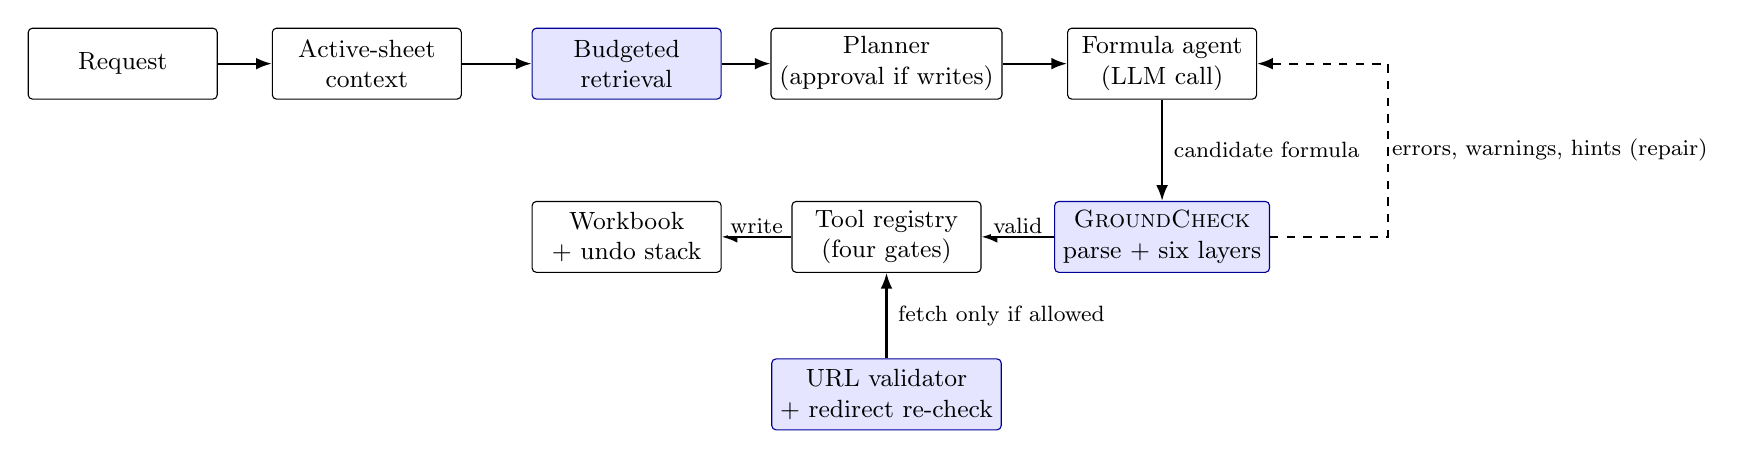
\begin{tikzpicture}[
  box/.style={draw, rounded corners=1.5pt, minimum height=9mm, minimum width=24mm, align=center, font=\small, inner sep=3pt},
  hl/.style={box, fill=blue!10, draw=blue!60!black},
  arr/.style={-{Latex[length=2mm]}, thick},
  lbl/.style={font=\footnotesize, fill=white, inner sep=1pt}
]
\node[box] (req) at (0,0) {Request};
\node[box] (ctx) at (3.1,0) {Active-sheet\\context};
\node[hl] (ret) at (6.4,0) {Budgeted\\retrieval};
\node[box] (plan) at (9.7,0) {Planner\\(approval if writes)};
\node[box] (agent) at (13.2,0) {Formula agent\\(LLM call)};
\node[hl] (ver) at (13.2,-2.2) {\gc\\parse + six layers};
\node[box] (tool) at (9.7,-2.2) {Tool registry\\(four gates)};
\node[box] (wb) at (6.4,-2.2) {Workbook\\+ undo stack};
\node[hl] (ssrf) at (9.7,-4.2) {URL validator\\+ redirect re-check};
\draw[arr] (req) -- (ctx);
\draw[arr] (ctx) -- (ret);
\draw[arr] (ret) -- (plan);
\draw[arr] (plan) -- (agent);
\draw[arr] (agent) -- (ver) node[lbl, midway, right=1mm] {candidate formula};
\draw[arr] (ver) -- (tool) node[lbl, midway, above] {valid};
\draw[arr] (tool) -- (wb) node[lbl, midway, above] {write};
\draw[arr] (ssrf) -- (tool) node[lbl, midway, right=1mm] {fetch only if allowed};
\draw[arr, dashed] (ver.east) -- ++(1.5,0) |- (agent.east) node[lbl, pos=0.25, right] {errors, warnings, hints (repair)};
\end{tikzpicture}}
\caption{Request flow. Shaded boxes are evaluated in this paper: retrieved cross-sheet context, the grounded verifier with its repair feedback, and the URL validator in front of the fetch tool.}
\label{fig:arch}
\end{figure*}


\subsection{Grounded verification (\gc)}
\label{sec:gc}
Each candidate formula is parsed into a typed AST by a small recursive-descent parser (the earlier verifier matched regular expressions against raw text) and checked in six deterministic layers that read only the open workbook:
\begin{enumerate}\itemsep0pt\topsep0pt
\item \textbf{Structural.} Leading \code{=}, balanced quotes and parentheses outside string literals, injection patterns, successful parse.
\item \textbf{Symbols.} Referenced sheets exist (case-insensitively, as in Sheets); a bare identifier is a function, named range or \code{LET}/\code{LAMBDA} variable (a header used as a name is rejected with the column's letters as a hint); function names within edit distance 1--2 of a real one are errors with ``did you mean'', other unknown names are warnings (custom functions); \code{QUERY} column letters exist.
\item \textbf{Bounds.} Each reference is checked against the extent of \emph{the sheet it points at}. A range wholly beyond the used columns is an error; one that merely extends past the last data row is headroom (a note); \code{COUNTA}, \code{COUNTBLANK} and \code{ISBLANK} may point at empty cells.
\item \textbf{Shape.} Argument counts for about 90 functions, lookup indices beyond the lookup range, literal \code{INDEX} positions, unequal range sizes in \code{SUMIFS}, \code{COUNTIFS}, \code{SUMIF}, \code{SUMPRODUCT}.
\item \textbf{Grounding.} Numeric aggregates over a text column; criteria and lookup keys that never occur in the column they search. The workbook proves neither impossible, so they are \emph{suspicious}: warnings with the column's real values as the hint, optionally sent to repair.
\item \textbf{Circularity.} The target cell lies inside a referenced range (\code{=SUM(F2:F81)} typed into F81, \code{=SUM(F:F)} into column F) or on a dependency chain through other formulas, where range dependencies are expanded to the formula cells inside them; \code{ROW}, \code{ROWS}, \code{COLUMN}, \code{COLUMNS} read only geometry and add no dependency.
\end{enumerate}
\begin{figure*}[!t]
\centering
\resizebox{\textwidth}{!}{%
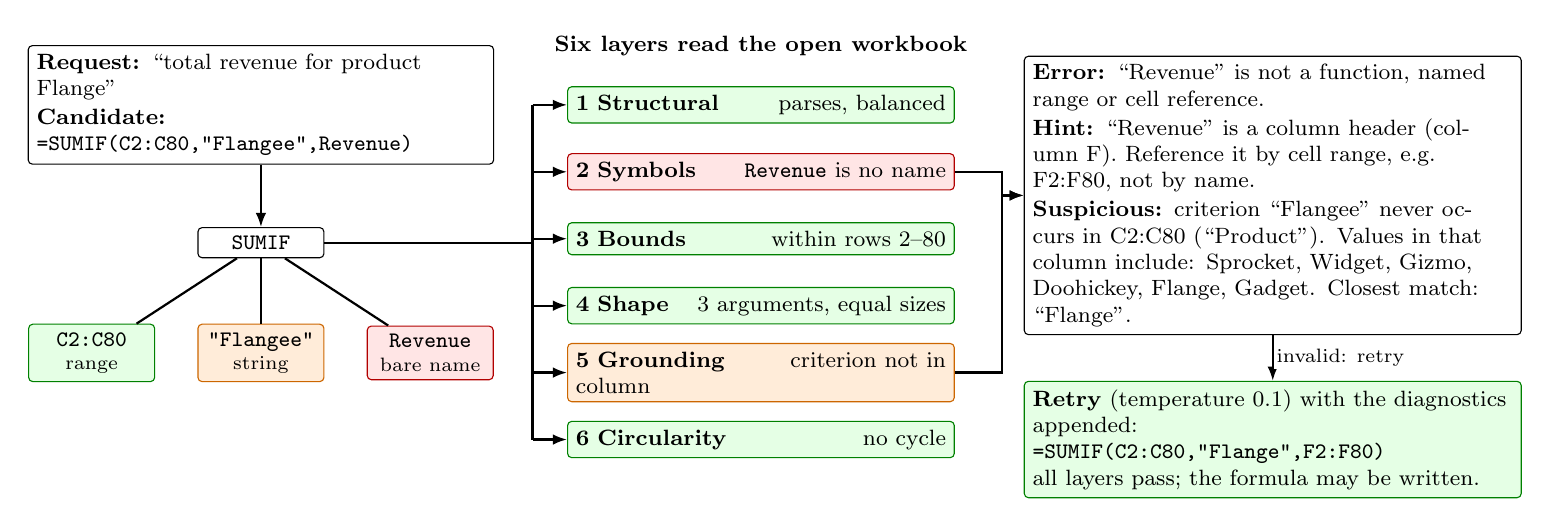
\begin{tikzpicture}[
  box/.style={draw, rounded corners=1.5pt, align=left, font=\footnotesize, inner sep=3pt},
  okb/.style={box, draw=green!50!black, fill=green!10},
  badb/.style={box, draw=red!70!black, fill=red!10},
  wrnb/.style={box, draw=orange!80!black, fill=orange!15},
  hl/.style={box, fill=blue!8, draw=blue!60!black},
  arr/.style={-{Latex[length=1.8mm]}, thick},
  lbl/.style={font=\scriptsize, fill=white, inner sep=1pt}
]
% candidate and its syntax tree
\node[box, text width=5.7cm] (req) at (2.85,0) {\textbf{Request:} ``total revenue for product Flange''\\[1pt]\textbf{Candidate:} \texttt{=SUMIF(C2:C80,"Flangee",Revenue)}};
\node[box, minimum width=1.6cm, align=center] (f) at (2.85,-1.75) {\texttt{SUMIF}};
\node[okb, align=center, minimum width=1.6cm] (a1) at (0.7,-3.15) {\texttt{C2:C80}\\[-1pt]\scriptsize range};
\node[wrnb, align=center, minimum width=1.6cm] (a2) at (2.85,-3.15) {\texttt{"Flangee"}\\[-1pt]\scriptsize string};
\node[badb, align=center, minimum width=1.6cm] (a3) at (5.0,-3.15) {\texttt{Revenue}\\[-1pt]\scriptsize bare name};
\draw[arr] (req) -- (f);
\draw[thick] (f) -- (a1); \draw[thick] (f) -- (a2); \draw[thick] (f) -- (a3);
% layers
\node[box, draw=none, font=\footnotesize\bfseries] at (9.2,0.75) {Six layers read the open workbook};
\node[okb, text width=4.7cm] (l1) at (9.2,0) {\textbf{1~Structural} \hfill parses, balanced};
\node[badb, text width=4.7cm] (l2) at (9.2,-0.85) {\textbf{2~Symbols} \hfill \texttt{Revenue} is no name};
\node[okb, text width=4.7cm] (l3) at (9.2,-1.7) {\textbf{3~Bounds} \hfill within rows 2--80};
\node[okb, text width=4.7cm] (l4) at (9.2,-2.55) {\textbf{4~Shape} \hfill 3 arguments, equal sizes};
\node[wrnb, text width=4.7cm] (l5) at (9.2,-3.4) {\textbf{5~Grounding} \hfill criterion not in column};
\node[okb, text width=4.7cm] (l6) at (9.2,-4.25) {\textbf{6~Circularity} \hfill no cycle};
\draw[thick] (f.east) -- (6.3,-1.75);
\draw[thick] (6.3,0) -- (6.3,-4.25);
\foreach \y/\n in {0/l1,-0.85/l2,-1.7/l3,-2.55/l4,-3.4/l5,-4.25/l6} \draw[arr] (6.3,\y) -- (\n.west);
% messages and retry
\node[box, text width=6.1cm] (msg) at (15.7,-1.15) {\textbf{Error:} ``Revenue'' is not a function, named range or cell reference.\\[1pt]\textbf{Hint:} ``Revenue'' is a column header (column~F). Reference it by cell range, e.g.\ F2:F80, not by name.\\[1pt]\textbf{Suspicious:} criterion ``Flangee'' never occurs in C2:C80 (``Product''). Values in that column include: Sprocket, Widget, Gizmo, Doohickey, Flange, Gadget. Closest match: ``Flange''.};
\node[okb, text width=6.1cm] (fix) at (15.7,-4.25) {\textbf{Retry} (temperature 0.1) with the diagnostics appended:\\\texttt{=SUMIF(C2:C80,"Flange",F2:F80)}\\ all layers pass; the formula may be written.};
\draw[arr] (l2.east) -- ++(0.6,0) |- (msg.west);
\draw[arr] (l5.east) -- ++(0.6,0) |- (msg.west);
\draw[arr] (msg.south) -- (fix.north) node[lbl, midway, right] {invalid: retry};
\end{tikzpicture}}
\caption{Worked example. The candidate formula mistypes a criterion and uses a column header as a name. GroundCheck parses it, reads the workbook's sheets, headers and column values, rejects it, and returns the column letter and the real values as repair feedback; the second attempt passes. The messages are the verifier's own output for a generated workbook (\texttt{eval/worked\_example.js}).}
\label{fig:anatomy}
\end{figure*}

Errors make a formula \emph{invalid} and trigger a retry (Figure~\ref{fig:anatomy} walks through an example). The verifier cannot know whether a formula answers the question: \code{=SUM(Quantity)} over the wrong numeric column is valid and wrong. After a failed attempt the formula and the layers' errors, warnings and hints (``Column ``Revenue'' is column D'', ``values in that column include East, West, North'') are appended to the conversation; temperature decays from 0.2 to 0.1 to 0 over at most two retries.

\subsection{What a workbook can decide}
\label{sec:levels}
A candidate formula can be wrong in ways that differ in how much of the workbook is needed to see it (Table~\ref{tab:levels}). Whether it parses, whether the names it uses exist, whether its ranges lie inside the data, whether its arguments fit the function, and whether it sits on a cycle can all be decided from the workbook alone. Whether a criterion matches the data can be decided only as a \emph{suspicion}, since a value missing from a column may be intended. Whether a valid formula answers the user's question cannot be decided without the user's intent: \code{=SUM(Quantity)} over the wrong numeric column parses, names real things, fits, is acyclic and matches the data. \gc{} works on the first five levels and leaves the last to the user. The experiments probe exactly this boundary, and we use the distinction between \emph{loud} faults (the cell shows an error) and \emph{silent} ones (a plausible but wrong value) to measure it.

\begin{table}
\caption{What a workbook can decide about a candidate formula, from syntax to intent, with the share of \sheetfault{} faults of that kind that each verifier blocks/flags (\%). The first four levels are decidable from the workbook alone; the data level is decidable only as a suspicion; whether a valid formula answers the question is not decidable without the user's intent.}
\label{tab:levels}

\centering\footnotesize
\begin{adjustbox}{max width=\columnwidth}\begin{tabular}{>{\raggedright\arraybackslash}p{3.7cm} c r cc}
\toprule
\textbf{Level of correctness} & \textbf{Decidable} & \textbf{n} & \textbf{Shipped} & \textbf{\gc} \\
\midrule
Syntax: does it parse? & yes & 3{,}173 & 100/100 & \textbf{100/100} \\
Names and extent: do the sheets, functions, headers and ranges it uses exist, within the data? & yes & 3{,}423 & 29/81 & \textbf{90/99} \\
Shape: do the arguments fit the function? & yes & 468 & 0/27 & \textbf{100/100} \\
Dependencies: is the target cell on a cycle? & yes & 4{,}320 & 40/60 & \textbf{100/100} \\
Data: do criteria and types match the column? & in part & 948 & 0/25 & \textbf{0/100} \\
Intent: does it compute what was asked? & no & 1{,}024 & 0/32 & \textbf{4/4} \\
\bottomrule
\end{tabular}\end{adjustbox}
\end{table}


\subsection{Retrieval and the fetch boundary}
\label{sec:retrieval}
A deterministic analyzer splits the workbook into tables with inferred types and statistics, builds a formula dependency graph, and emits one chunk per table listing each column's \emph{letter}, type and statistics and the data-row span (a first version listed headers only; Section~\ref{sec:e5} shows why that failed). Seven signals score chunks against the request (active sheet, referenced by the active cell's formula, lexical overlap, shared headers, neighbouring table, graph proximity, conversation overlap) and a greedy knapsack fills a token budget. In the original add-on this context reached the planner but not the formula agent; we pass it on.

As a secondary component, the same idea of checking before acting applies where an LLM-chosen string leaves the add-on, the fetch tool, the setting of server-side request forgery (SSRF)~\cite{owaspssrf}. The original filter matched regular expressions against the whole URL. Our validator parses it and classifies the \emph{host}: IPv4 in any \code{inet\_aton} form, IPv6 including IPv4-mapped, NAT64 and 6to4, the reserved ranges of RFC~6890~\cite{rfc6890}, single-label and internal-only names, wildcard-DNS services, embedded credentials, and characters on which URL parsers disagree. Redirects are not auto-followed: every hop is re-validated. A static check cannot see DNS rebinding.

\section{Evaluation Design}
\label{sec:method}

The add-on's source files run as shipped in a sandbox that stubs only the Apps Script globals. Every generator is seeded. Four questions structure the evaluation: how much of a benchmark's failure the checks stop (RQ1), whether this carries over to formulas people actually wrote (RQ2), whether verification-guided repair helps real models (RQ3), and whether repair makes failures safer or only less visible (RQ4).

\subsection{\sheetfault}
\label{sec:benchmark}
\begin{figure*}[!t]
\centering
\resizebox{\textwidth}{!}{%
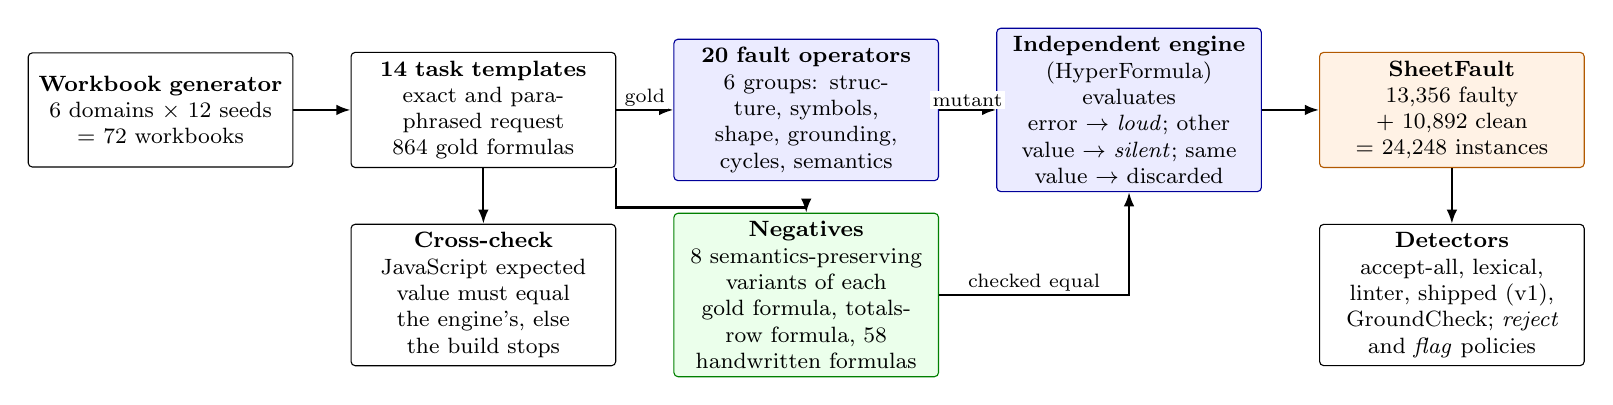
\begin{tikzpicture}[
  box/.style={draw, rounded corners=1.5pt, align=center, font=\footnotesize, inner sep=3pt, text width=3.15cm, minimum height=1.45cm},
  hl/.style={box, fill=blue!8, draw=blue!60!black},
  neg/.style={box, fill=green!8, draw=green!50!black},
  outb/.style={box, fill=orange!10, draw=orange!70!black},
  arr/.style={-{Latex[length=1.8mm]}, thick},
  lbl/.style={font=\scriptsize, fill=white, inner sep=1pt}
]
\node[box] (wb) at (0,0) {\textbf{Workbook generator}\\6 domains $\times$ 12 seeds\\= \nBenchWorkbooks{} workbooks};
\node[box] (task) at (4.1,0) {\textbf{14 task templates}\\exact and paraphrased request\\\nBenchGold{} gold formulas};
\node[hl] (flt) at (8.2,0) {\textbf{\nBenchClasses{} fault operators}\\6 groups: structure, symbols,\\shape, grounding, cycles, semantics};
\node[hl] (eng) at (12.3,0) {\textbf{Independent engine}\\(HyperFormula) evaluates\\error $\to$ \emph{loud}; other value $\to$ \emph{silent}; same value $\to$ discarded};
\node[outb] (bm) at (16.4,0) {\textbf{SheetFault}\\\nBenchFaults{} faulty\\+ \nBenchClean{} clean\\= \nBenchTotal{} instances};
\node[neg] (var) at (8.2,-2.35) {\textbf{Negatives}\\8 semantics-preserving variants of each gold formula, totals-row formula, 58 handwritten formulas};
\node[box] (det) at (16.4,-2.35) {\textbf{Detectors}\\accept-all, lexical, linter, shipped (v1), GroundCheck; \emph{reject} and \emph{flag} policies};
\node[box] (chk) at (4.1,-2.35) {\textbf{Cross-check}\\JavaScript expected value must equal the engine's, else the build stops};
\draw[arr] (wb) -- (task);
\draw[arr] (task) -- (flt) node[lbl, midway, above] {gold};
\draw[arr] (flt) -- (eng) node[lbl, midway, above] {mutant};
\draw[arr] (eng) -- (bm);
\draw[arr] (task.south) -- (chk.north);
\draw[arr] (task.south east) -- ++(0,-0.5) -| (var.north);
\draw[arr] (var.east) -| (eng.south) node[lbl, pos=0.25, above] {checked equal};
\draw[arr] (bm) -- (det);
\end{tikzpicture}}
\caption{Construction of \sheetfault. Labels come from an independent spreadsheet engine, never from the verifier under test; mutants that preserve the value are discarded as equivalent, and semantics-preserving variants are checked against the engine before they are used as negatives.}
\label{fig:bench}
\end{figure*}

\paragraph{Workbooks, tasks and gold formulas}
Figure~\ref{fig:bench} summarises how the benchmark is built. A seeded generator produces workbooks from \accDomains{} domains (a main table of 24--120 rows, a lookup sheet, a summary sheet with live formulas, and in 40\% of workbooks a named range), \accSeeds{} seeds per domain, so \accDomains{} $\times$ \accSeeds{} = \accWorkbooks{} workbooks. For each workbook, \accTasksPerWb{} tasks are drawn with replacement from a weighted pool of 14 templates (aggregates, conditional sums and counts, \code{SUMIFS}, cross-sheet lookups, ratios, ranks, \code{INDEX/MATCH}), giving \accWorkbooks{} $\times$ \accTasksPerWb{} = \accGold{} gold formulas. Each task has a request in two forms, one with the exact header words and one paraphrased with no shared word, a gold formula, and an expected value computed in JavaScript. We require it to agree with HyperFormula~\cite{hyperformula}, an independent open-source engine; the build stops at the first disagreement, and all \nBenchGold{} gold formulas pass.

\paragraph{Faults and labels}
Twenty operators in six groups corrupt a gold formula (Appendix~\ref{app:bench}): structural damage, hallucinated symbols, shape errors, ungrounded values and types, circular references, and two \emph{semantic} swaps (wrong numeric column, wrong aggregation) that yield valid formulas answering another question. The labels use information independent of the verifier under test. A candidate is \emph{faulty} if the engine returns an error or a value different from gold; it is \emph{loud} if the engine returns an error and \emph{silent} if it returns a plausible wrong value. A mutation that preserves the value by coincidence is an \emph{equivalent mutant} and is discarded. The \code{QUERY} class is labelled by construction, since HyperFormula has no \code{QUERY}. HyperFormula follows Excel, not Google Sheets; Section~\ref{sec:limitations} and Appendix~\ref{app:gsheets} describe how far that matters and the harness for checking it in Google Sheets itself.

\paragraph{Negatives, accounting and detectors}
The \nBenchClean{} clean instances are \accGold{} gold formulas, \accVariants{} semantics-preserving variants (eight kinds, such as absolute and whole-column references, lowercase, spacing, own-sheet prefix, \code{IFERROR}, named range and headroom, each kept only if the engine confirms it equal to gold), \accTotals{} ordinary totals-row formulas (\accCircPerWb{} per workbook), \accQuery{} valid \code{QUERY} formulas (\accQueryPerWb{} per workbook), and \accExtra{} + \accCustom{} handwritten formulas exercising syntax a parser must accept, \accHandPerWb{} per workbook, two of which call a custom function. The \nBenchFaults{} faults are the per-class counts of Table~\ref{tab:e1-classes}: each operator is applied once to each gold formula it applies to (counts below \accGold{} are operators that do not apply to every formula, for example the unbalanced-quote operator needs a string literal), and the circular and \code{QUERY} classes are generated per workbook. In all, \nBenchTotal{} instances over \nBenchWorkbooks{} workbooks. We compare accepting everything; a lexical check; a linter that also rejects functions outside the official Sheets list~\cite{googlefunctions}; the verifier shipped at commit \code{44a3f4f} (``v1''); and \gc. \emph{Reject} counts a detection only if the formula is blocked, \emph{flag} also counts warnings; the false-positive rate (FPR) is measured on the clean set under the same policy.

\subsection{Real-world formulas}
\label{sec:rwmethod}
From Sheetpedia~\cite{tian2025sheetpedia} (Enron, FUSE, forum files) we draw three disjoint sets of 300 workbooks that load, have formulas, and are at most 600\,kB, 1{,}500 rows, 60 columns and 12 sheets, shuffled with a fixed seed. Up to 25 formulas per workbook (no structured or external references) are verified in their own workbook with the target cell emptied. The \emph{development} set came from the first 500\,MB of the release archive and was inspected while fixing the verifier. The \emph{held-out} set came from the same part and was scored once, after which one verifier change was made (Section~\ref{sec:e1b}); its first-pass figures are the ones reported. The \emph{confirmation} set came from a later part of the archive (after the first 540\,MB), so it is disjoint from both. Its protocol was fixed before the data were fetched: the SHA-256 of the verifier sources was recorded, and the scoring script refuses to run if they change. \ifdefined\rwcGFormulas After this run exposed two defect classes and the verifier was extended (Section~\ref{sec:e1b}), a \emph{second confirmation} set from a yet later part of the archive was scored once with the new version, frozen in the same way.\fi{} The release carries no cached results, so there are no labels: we report rejection rates, group the reasons, and use HyperFormula's evaluation of the original formula as supporting evidence. We claim no precision figure.

\subsection{End-to-end study}
\label{sec:e5method}
We draw 360 tasks (24 workbooks, 15 tasks each, from the same 14 templates) and run the production formula agent against two open-weight models, Llama~3.1 8B and Llama~3.2 3B~\cite{dubey2024llama3} (4-bit quantized, served by Ollama), and three hosted models through the Gemini API: Gemini~3.1 Flash-Lite, 3.5 Flash-Lite, and the open-weight Gemma~4 26B-A4B (a 1{,}024-token output cap, a low or minimal thinking level, and the add-on's own request otherwise). Every hosted response carries the model version the API reports, and the result files store it with each task; in every hosted run it equals the requested identifier (\efDVersionMatch{} of \efDVersionCalls{} responses for \efDName, \efEVersionMatch{} of \efEVersionCalls{} for \efEName, \efFVersionMatch{} of \efFVersionCalls{} for \efFName). An earlier pilot requested \code{gemini-3.1-flash-lite-preview}, an identifier Google lists as retired on 25 May 2026; the API still answered it on 2 October 2026, reporting \code{gemini-3.1-flash-lite}, but the pilot did not log versions, so it is not used. Only \code{UrlFetchApp.fetch} is replaced, by a stub that forwards the add-on's Gemini-format request or translates it for Ollama. A candidate is \emph{correct} if HyperFormula evaluates it at the target cell without error to the gold value. Attempt 1 is generated with the shipped active-sheet context (\emph{flat}) and with ranked cross-sheet context added (\emph{retrieved}), in the chunk format shipped before and after column letters were added. From the retrieved attempt 1, up to two repair attempts are forked under five strategies that differ only in the feedback: \emph{resample} (same prompt, no feedback), \emph{generic} (``your formula was invalid, try again''), \emph{v1 feedback}, \emph{\gc{} feedback}, and \emph{\gc{} + suspicious}, which also repairs on suspicious findings. The local models were run with three sampling seeds; hosted models with one. Because the chunk fix followed the first pass, we confirm the final system on 180 tasks from fresh workbooks. Separately, a critic baseline asks the same model, with the same context, whether a formula is VALID or INVALID, on a stratified sample of \sheetfault.

\subsection{Statistics and metrics}
\label{sec:statsmethod}
Benchmark instances share workbooks, so they are not independent. We report workbook-clustered intervals (a bootstrap over the \accWorkbooks{} workbooks, 2{,}000 resamples) next to formula-level Wilson intervals~\cite{wilson1927}, and the same bootstrap over the 300 workbooks of each real-world set. End-to-end comparisons are paired by task: exact McNemar tests~\cite{mcnemar1947}, Holm-adjusted within each model over the four feedback strategies, and paired bootstrap intervals; with several seeds each task's outcome is first averaged over the seeds and the bootstrap runs over tasks. Beyond accuracy we measure what ends up in the cell. A \emph{silent} cell holds a plausible but wrong value, the failure a user cannot see. The \emph{unsafe-repair rate} of a strategy is the share of rejected first attempts whose repaired formula is valid but wrong, that is, repair has turned a visible failure into an invisible one.

\subsection{Retrieval, cost and security}
\emph{Retrieval}: workbooks with about 10 tables plus 0, 10 or 30 distractor tables with overlapping headers; requests are aggregates (A), lookups (B) and ``change \emph{this} formula'' (C, nothing named), with the column named (H) or paraphrased (S); a request is gold-complete if the prompt holds \emph{every} table a correct formula reads; baselines are BM25~\cite{robertson2009bm25}, lexical-only and graph-only variants, random, and the active sheet alone. \emph{Cost}: \code{SpreadsheetApp} calls (each a round trip on Apps Script) and Node CPU time as workbooks grow. \emph{SSRF} (a secondary component): URLs that must be blocked (private, loopback, link-local and metadata addresses in every encoding a resolver accepts, IPv6 forms, authority tricks, internal names, non-HTTP schemes) and URLs that must be allowed (public hosts, addresses next to private ranges, benign URLs containing suspicious substrings).

\section{Results}
\label{sec:results}

\subsection{Fault detection on \sheetfault}
\label{sec:e1}
\begin{table*}[!t]
\caption{Fault detection on \textsc{SheetFault} (13{,}356 faulty and 10{,}892 clean formulas, micro-averaged, \%). \emph{Reject} counts a formula as detected only if it is blocked; \emph{flag} also counts warnings. FPR is the share of clean formulas that is rejected or flagged.}
\label{tab:e1-overall}

\centering\footnotesize
\begin{tabular}{l rrrr rrrr}
\toprule
& \multicolumn{4}{c}{\textbf{Reject policy} (block on error)} & \multicolumn{4}{c}{\textbf{Flag policy} (error or warning)} \\
\cmidrule(lr){2-5}\cmidrule(lr){6-9}
\textbf{Detector} & P & R & F1 & FPR & P & R & F1 & FPR \\
\midrule
Accept all & -- & 0.0 & -- & 0.0 & -- & 0.0 & -- & 0.0 \\
Syntax only & 100.0 & 17.6 & 29.9 & 0.0 & 100.0 & 17.6 & 29.9 & 0.0 \\
Linter & 96.2 & 27.2 & 42.4 & 1.3 & 96.2 & 27.2 & 42.4 & 1.3 \\
Shipped (v1) & 100.0 & 44.2 & 61.3 & 0.0 & 85.2 & 69.2 & 76.4 & 14.7 \\
GroundCheck & \textbf{100.0} & \textbf{83.0} & \textbf{90.7} & 0.0 & \textbf{98.8} & \textbf{92.4} & \textbf{95.5} & 1.3 \\
\bottomrule
\end{tabular}
\end{table*}


A lexical check blocks only \eonesyntaxrejectR\% of faults and a function linter \eonelintrejectR\% (Table~\ref{tab:e1-overall}): most benchmark faults are well formed and name things that do not exist or do not fit the data. The shipped verifier blocks \eonevonerejectR\% (F1 \eonevonerejectF) with no false positives, but \eonevoneflagR\% only if warnings count, and then \eonevoneflagFPR\% of clean formulas are flagged: its row-bounds warning fires on every formula with headroom (\cleanHeadroomVone\% of those) and its function list omits common functions such as \code{AVERAGEIF} and \code{MAXIFS}, so \cleanGoldVone\% of the \emph{gold} formulas are flagged. \gc{} blocks \eonevtworejectR\% (F1 \eonevtworejectF) at \eonevtworejectFPR\% false positives; counting warnings, recall is \eonevtwoflagR\% at FPR \eonevtwoflagFPR\%, and every flagged clean formula is a custom function missing from the official list (a warning by design; Table~\ref{tab:e1-clean}, Appendix~\ref{app:bench}, gives the false-alarm rate for every clean class).

The headline difference is large and does not depend on how uncertainty is counted. Resampling the \clWbN{} workbooks rather than the formulas gives a 95\% interval of [\clVtwoRecallLo, \clVtwoRecallHi]\% for the recall of \gc{} and [\clVoneRecallLo, \clVoneRecallHi]\% for the shipped verifier, a paired difference of \clDiffRecall{} points [\clDiffRecallLo, \clDiffRecallHi], and \gc{} is ahead in \clWbBetter{} of \clWbN{} workbooks. These intervals are narrow because one generator produces every workbook, so they measure sampling noise, not how representative the benchmark is. The benchmark was written with the verifier; Section~\ref{sec:e1b} tests it on real formulas.

Figure~\ref{fig:e1-classes} and Table~\ref{tab:e1-classes} (Appendix~\ref{app:results}) show where the gain comes from. The shipped verifier cannot see a range that contains its own cell (\clsrangecontainsselfvoneReject\% blocked), a whole-column self-inclusion (\clscolumncontainsselfvoneReject\%), a cycle through a range (\clscycleindirectrangevoneReject\%), a header used as a name (\clsheaderasnamevoneReject\%), unequal range sizes (\clsrangesizemismatchvoneReject\%) or an out-of-range lookup index (\clslookupindexoobvoneReject\%): its graph links a range to one node, never to the formula cells inside it, so the totals-row mistake is invisible. \gc{} blocks all of them. Hallucinated function names are blocked only as near-misses (\clsghostfunctionvtwoReject\%) and otherwise warned about (\clsghostfunctionvtwoFlag\% flagged), as intended for a language with custom functions; an absent criterion and an aggregate over text are flagged (\clsghostvaluevtwoFlag\% and \clstypemismatchvtwoFlag\%) but never rejected; the two semantic classes (\clswrongnumericcolN{} and \clswrongfunctionN{} instances) are essentially undetectable, as they must be.

\begin{figure}[t]
\centering
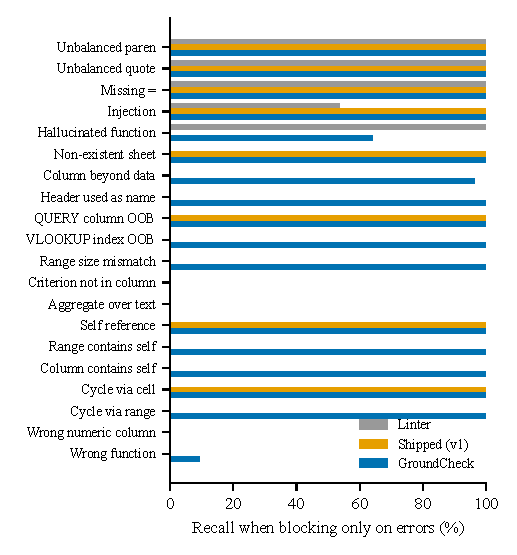
\includegraphics[width=0.95\columnwidth]{figures/fig_e1_classes}
\caption{Recall per fault class when a formula is blocked only on errors.}
\label{fig:e1-classes}
\end{figure}

\begin{table}
\caption{Leave-one-layer-out ablation of the verifier on \textsc{SheetFault} (\%).}
\label{tab:e1-ablation}

\centering\footnotesize
\begin{adjustbox}{max width=\columnwidth}\begin{tabular}{l rr rr}
\toprule
& \multicolumn{2}{c}{\textbf{Reject}} & \multicolumn{2}{c}{\textbf{Flag}} \\
\cmidrule(lr){2-3}\cmidrule(lr){4-5}
\textbf{Configuration} & R & F1 & R & F1 \\
\midrule
All layers & 83.0 & 90.7 & 92.4 & 95.5 \\
$-$ structural + parse & 62.4 & 76.9 & 71.9 & 83.1 \\
$-$ symbols & 66.5 & 79.9 & 73.6 & 84.8 \\
$-$ bounds & 78.5 & 87.9 & 87.9 & 93.0 \\
$-$ shape & 79.2 & 88.4 & 88.6 & 93.4 \\
$-$ grounding & 83.0 & 90.7 & 85.3 & 91.5 \\
$-$ circularity & 50.6 & 67.2 & 66.5 & 79.4 \\
$-$ QUERY columns & 81.9 & 90.1 & 91.3 & 94.9 \\
\bottomrule
\end{tabular}\end{adjustbox}
\end{table}


Removing one layer at a time (Table~\ref{tab:e1-ablation}), circularity matters most (reject recall \eonevtworejectR\% $\to$ \ablcircularRejectR\%), then the parse (\ablstructuralRejectR\%) and symbols (\ablsymbolsRejectR\%). Grounding leaves reject recall unchanged because its findings are warnings. Of the \visloudN{} loud faults \gc{} blocks \visloudvtwoReject\% (shipped: \visloudvoneReject\%); of the \vissilentN{} silent faults, which would write a plausible wrong value into the sheet, it blocks \vissilentvtwoReject\% and flags \vissilentvtwoFlag\% (shipped: \vissilentvoneReject\% and \vissilentvoneFlag\%; Figure~\ref{fig:e1-visibility}). The rest are the semantic swaps: verification turns most silent failures into visible ones but does not make an agent correct.

\begin{figure}[t]
\centering
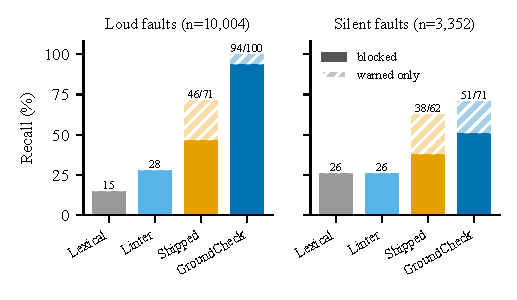
\includegraphics[width=\columnwidth]{figures/fig_e1_visibility}
\caption{Recall on loud and silent faults. Solid: the formula is blocked; hatched: only a warning is raised.}
\label{fig:e1-visibility}
\end{figure}

The result does not depend on the workbook domain (Figure~\ref{fig:e1-domain}): reject recall is \domVtwoMin--\domVtwoMax\% for \gc{} and \domVoneMin--\domVoneMax\% for the shipped verifier in each of the six domains, with \domVtwoFPRMax\% false positives in every one; across the \domWbN{} individual workbooks it ranges from \domWbMin\% to \domWbMax\% (shipped: \domWbVoneMin--\domWbVoneMax\%), so no single workbook accounts for the gain.

\begin{figure}[t]
\centering
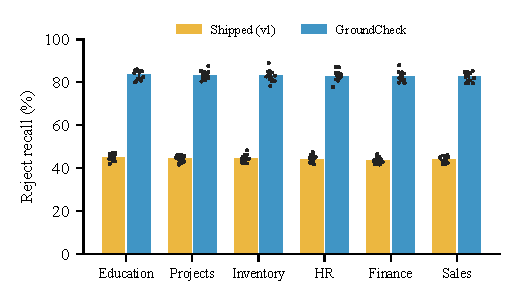
\includegraphics[width=\columnwidth]{figures/fig_e1_domain}
\caption{Reject recall by workbook domain, with 95\% Wilson intervals; each dot is one of the 12 workbooks of the domain.}
\label{fig:e1-domain}
\end{figure}

\subsection{Real-world formulas}
\label{sec:e1b}
\paragraph{Development and held-out sets}
On the development set the first runs exposed two defects in our verifier, a tokenizer gap for row ranges with absolute markers (\code{\$1:\$1}) and a circularity false positive on \code{ROWS(B\$2:B83)} placed in B83, and one in our corpus extraction (Excel defined names were not loaded). After fixing them the development rejection rate is \rwDevvtwoReject\% (shipped verifier: \rwDevvoneReject\%). The held-out set, scored once, gives \rwcTVoneReject\% for the shipped verifier and \rwcTVtwoReject\% for \gc{} on \rwcTFormulas{} formulas from \rwcTWorkbooks{} workbooks (flag policy: \rwvoneFlag\% and \rwvtwoFlag\%). After seeing it we exempted \code{COUNTA}, \code{COUNTBLANK} and \code{ISBLANK} when they point at empty cells, which lowers the rate to \rwvtwoRejectPost\%; the first-pass figure is the held-out result, because the second was tuned on this set.

By rejection rate the two verifiers are not distinguishable: the difference is \rwcTDiff{} points (workbook-clustered 95\% interval [\rwcTDiffLo, \rwcTDiffHi]; Table~\ref{tab:rw-sets}). Rejections are concentrated. Only \rwcTWbRejected{} of the 300 workbooks contain a rejection of a real formula, and the five workbooks with the most rejections hold \rwcTTopfiveShare\% of them, which is why these intervals are far wider than formula-level ones.

\begin{table}
\caption{Share of real-world formulas (\%) rejected, with 95\% intervals from a bootstrap over workbooks (300 workbooks per set). Rejections are concentrated in a few workbooks, so these intervals are much wider than formula-level ones.}
\label{tab:rw-sets}

\centering\footnotesize
\begin{adjustbox}{max width=\columnwidth}\begin{tabular}{l r c c}
\toprule
\textbf{Set} & \textbf{Formulas} & \textbf{Shipped} & \textbf{\gc} \\
\midrule
Held-out, before the change & 5{,}184 & 8.8 [5.8, 12.1] & 8.6 [5.6, 11.8] \\
Confirmation 1, frozen v2 & 5{,}537 & 9.0 [5.6, 12.3] & 10.4 [6.8, 13.9] \\
Confirmation 2, frozen v2.1 & 5{,}277 & 6.4 [3.9, 9.2] & 7.6 [4.8, 10.5] \\
\bottomrule
\end{tabular}\end{adjustbox}
\end{table}


\begin{figure}[t]
\centering
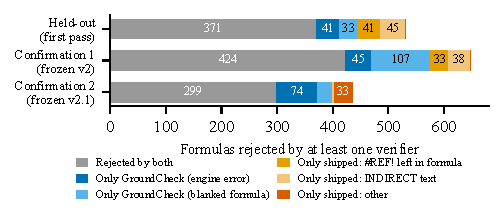
\includegraphics[width=\columnwidth]{figures/fig_rw_overlap}
\caption{Where the two verifiers disagree on real formulas: the formulas rejected by at least one of them, by who rejects them. Formulas blanked by the dataset's PII pass count as artifacts. Confirmation set~2 was scored with the extended verifier.}
\label{fig:rw-overlap}
\end{figure}

\paragraph{Confirmation set, verifier frozen}
The confirmation set (\rwcFFormulas{} formulas from \rwcFWorkbooks{} workbooks), scored once with the frozen verifier, gives \rwcFVoneReject\% for the shipped verifier and \rwcFVtwoReject\% for \gc{}, a difference of \rwcFDiff{} points [\rwcFDiffLo, \rwcFDiffHi]. Of the \rwcFRejected{} rejections by \gc, \rwcFEmpty{} are formulas that the dataset's PII pass blanked to \code{=}; they are not real formulas, and without them the rate is \rwcFVtwoRejectNoEmpty\% [\rwcFVtwoRejectNoEmptyLo, \rwcFVtwoRejectNoEmptyHi]. For \rwcFEngineConfirmedReal{} of the other \rwcFRealRejected{} the independent engine also returns an error (Appendix~\ref{app:results}). Most of the rest reference sheets that do not exist, \rwcFGhostOkMasked{} of them inside \code{IFERROR} or a similar wrapper: the formula is broken and the wrapper hides it, a latent fault that no check on values can see.

The sets show where the two verifiers differ (Figure~\ref{fig:rw-overlap}). Both reject \rwcFOBoth{} formulas. Only \gc{} rejects \rwcFOOnlyVtwoReal{} real formulas (the engine returns an error for \rwcFOOnlyVtwoEngineError{} of them), chiefly circular references and ranges beyond the data. Only the shipped verifier rejects \rwcFOOnlyVone{}. \rwcFOOnlyVoneRefLiteral{} of them contain a literal \code{\#REF!}, a reference deleted from the formula, which the shipped verifier catches by accident because it reads \code{REF!} as a sheet name; \rwcFOOnlyVoneIndirect{} are \code{INDIRECT} calls whose text names a sheet that does not exist, or builds the name by concatenation; these are \gc's misses. The remaining \rwcFOOnlyVoneOther{} is a parsing error of the shipped verifier on a sheet name that contains a quote. Neither class is in \sheetfault, and \gc{} checked neither: a benchmark written with the verifier cannot show a gap that the authors' idea of faults did not include. The held-out set held the same gap (\rwcTORefLiteralInAnyFormula{} formulas with \code{\#REF!}), which we had not examined from this angle. Deleted references are not rare: \rwcFORefLiteralInAnyFormula{} of \rwcFFormulas{} confirmation formulas contain one.

\ifdefined\rwcGFormulas
\paragraph{Closing the gap, and a second confirmation}
We extended \gc{} by two rules: a literal \code{\#REF!} or \code{\#NAME?} in a formula is an error, and an \code{INDIRECT} whose text starts with a sheet name is checked against the workbook's sheets. The rules change none of the \eqInstances{} \sheetfault{} verdicts (\eqDiff{} differ) and can fire on none of the \eqFormulas{} formulas the models generated (\eqHits{} do), so the benchmark and end-to-end results hold for the extended verifier. Scored again on the real formulas, the extended verifier rejects \rwcTPVtwoReject\% of the held-out and \rwcFPVtwoReject\% of the confirmation formulas, but these figures are post hoc, since both sets informed the rules. The confirmatory test is a second confirmation set (\rwcGFormulas{} formulas from \rwcGWorkbooks{} workbooks, from a later part of the archive), scored once with the extended verifier frozen: the shipped verifier rejects \rwcGVoneReject\% and \gc{} \rwcGVtwoReject\% (difference \rwcGDiff{} points [\rwcGDiffLo, \rwcGDiffHi]; without blanked formulas \rwcGVtwoRejectNoEmpty\%). Of the \rwcGOOnlyVone{} formulas that only the shipped verifier rejects, \rwcGOOnlyVoneRefLiteral{} contain \code{\#REF!}; reading all of them, the rest are spurious rejections: it takes parentheses and \code{!} inside text literals for code, and treats an \code{INDIRECT} whose sheet name comes from a named range as a missing sheet (the engine evaluates \rwcGOOnlyVoneEngineOk{} of them without error). The \rwcGOOnlyVtwoReal{} real formulas that only \gc{} rejects all produce an engine error (\rwcGOOnlyVtwoEngineError{}).
\fi

Taken together, between about 6\% and 11\% of real formulas are rejected by either verifier, the rejections sit in a few workbooks, and \gc{} rejects one to two points more than the shipped verifier, a difference whose workbook-clustered interval includes zero in every set. The larger gain that \sheetfault{} shows does not appear in the rejection rate on real formulas. What differs is the kind of rejection. Where the verifiers disagree, the formulas that only \gc{} rejects are engine-confirmed errors (\rwcFOOnlyVtwoEngineError{} of \rwcFOOnlyVtwoReal{} in confirmation set~1\ifdefined\rwcGFormulas, \rwcGOOnlyVtwoEngineError{} of \rwcGOOnlyVtwoReal{} in set~2\fi)\ifdefined\rwcGFormulas, and, once deleted references are covered, the \rwcGOOnlyVone{} formulas that only the shipped verifier rejects in set~2 are all spurious\fi. This is supporting evidence, not a precision figure, since it rests on one engine and on our reading of the formulas. The benchmark measures coverage of the fault classes we designed; real formulas contain some of them rarely and others, such as deleted references, that we had not listed.

\subsection{End-to-end accuracy with real models}
\label{sec:e5}
We run the production formula agent with two local models, \efAName{} and \efBName, and three hosted ones, \efDName, \efEName{} and \efFName{} (Section~\ref{sec:e5method}). With the final system the first attempt is correct for \efAfinal\% of the \efAN{} tasks with \efAName{} and \efBfinal\% with \efBName; the hosted models reach \efDfinal\% (\efDN{} tasks), \efEfinal\% (\efEN) and \efFfinal\% (\efFN).

\paragraph{Retrieved context needs column letters}
\begin{table}
\caption{Attempt-1 execution accuracy (\%) by context. Lookup tasks read a sheet other than the active one; ``Other'' tasks read the active sheet only. The only difference between the two retrieved rows is that table chunks now carry column letters and the data-row span.}
\label{tab:e5-context}

\centering\footnotesize
\begin{adjustbox}{max width=\columnwidth}\begin{tabular}{l l rrr}
\toprule
\textbf{Model} & \textbf{Context} & \textbf{All} & \textbf{Lookup} & \textbf{Other} \\
\midrule
\multirow{3}{*}{Llama~3.1 8B} & Active sheet only & 72.2 & 3.3 & 78.5 \\
 & Retrieved (shipped) & 64.4 & 0.0 & 70.3 \\
 & Retrieved + letters & \textbf{70.8} & 0.0 & 77.3 \\
\midrule
\multirow{2}{*}{Llama~3.2 3B} & Active sheet only & 37.5 & 3.3 & 40.6 \\
 & Retrieved + letters & \textbf{38.9} & 3.3 & 42.1 \\
\midrule
\multirow{2}{*}{Llama~3.1 8B, new tasks} & Active sheet only & 76.7 & 0.0 & 80.7 \\
 & Retrieved + letters & \textbf{72.2} & 0.0 & 76.0 \\
\midrule
\multirow{2}{*}{Gemini~3.1 Flash-Lite} & Active sheet only & 89.2 & 31.8 & 95.0 \\
 & Retrieved + letters & \textbf{96.7} & 95.5 & 96.8 \\
\midrule
\multirow{2}{*}{Gemini~3.5 Flash-Lite} & Active sheet only & 89.9 & 27.3 & 96.0 \\
 & Retrieved + letters & \textbf{95.2} & 95.5 & 95.1 \\
\midrule
\multirow{2}{*}{Gemma~4 26B-A4B} & Active sheet only & 91.1 & 36.7 & 96.1 \\
 & Retrieved + letters & \textbf{95.8} & 96.7 & 95.8 \\
\bottomrule
\end{tabular}\end{adjustbox}
\end{table}

With the shipped active-sheet context \efAName{} reaches \efAflat\% at attempt 1 (Table~\ref{tab:e5-context}). Adding the ranked context in the chunk format the add-on shipped \emph{lowered} accuracy to \efAshipped\% (\efATestshippedvsflatB{} tasks favour the active sheet alone, \efATestshippedvsflatA{} the retrieved context; $p$ \efATestshippedvsflatP, exact McNemar). Those chunks listed columns by header only, so the model guessed letters (a silently wrong numeric column), wrote headers as names (\code{COUNTIF(Lead Time,">31")}) or invented functions. With each column's letter and the data-row span in the chunk, accuracy is \efAfinal\% ($p$ \efATestfinalvsshippedP{} against the shipped format), indistinguishable from the active sheet alone ($p$ \efATestfinalvsflatP): retrieval does not help on tasks that read the active sheet; its purpose is cross-sheet requests. There the first attempt is correct \efAfinalLookup\% of the time on the \efAfinalLookupN{} lookup tasks, because of the prompt rather than the context: \efALkSheetTwo{} of \efALkN{} attempts copied \code{Sheet2} from the agent's own worked example (Section~\ref{sec:discussion}). For the hosted models the retrieved context is what matters: it raises accuracy from \efDflat\%, \efEflat\% and \efFflat\% with the active sheet alone to \efDfinal\%, \efEfinal\% and \efFfinal\%, almost entirely on cross-sheet lookups (\efDflatLookup\% to \efDfinalLookup\% for \efDName).
\ifdefined\efCN
\emph{Held-out confirmation.} On \efCN{} tasks from fresh workbooks the final chunk format gives \efCfinal\% at attempt 1 against \efCflat\% for the active sheet alone ($p$ \efCTestfinalvsflatP), the same picture as on the main set. \gc{} feedback raises it to \efCSvtwofb\% ($+$\efCSvtwofbD{} points, Holm-adjusted $p$ \hmCHolmVtwoRes{} against resampling) and, with suspicious findings, to \efCSvtwofbplussusp\% ($p$ \hmCHolmSuspRes): the same direction with less power.
\fi

\paragraph{What verification sees}
Of the \efAWrong{} formulas \efAName{} gets wrong at attempt 1, \efALoud{} (\efALoudShare\%) are loud and \efASilent{} are silent (Figure~\ref{fig:e5-taxonomy}; Table~\ref{tab:e5-taxonomy}, Appendix~\ref{app:results}). \gc{} rejects \efACaughtTwo{} of them (the shipped verifier \efACaughtOne{}) and flags \efAFlagTwo{} in all; it rejects none of the silent ones and flags \efASilentFlagTwo{}. None of the \efANCorrect{} correct formulas is rejected. The rejections are concentrated: 29 of the 35 are references to a sheet that does not exist (the \code{Sheet2} copies), which both verifiers catch, so the large recall gap of Section~\ref{sec:e1} does not appear here; the natural faults of these models fall mostly in classes that the shipped verifier already handles. Using the verifier as an acceptance gate, the \efAGateAccN{} accepted formulas are correct \efAGateAcc\% of the time and the \efAGateRejN{} rejected ones \efAGateRej\%. The hosted models make \efDWrong, \efEWrong{} and \efFWrong{} wrong first attempts; \gc{} rejects \efDCaughtTwo, \efECaughtTwo{} and \efFCaughtTwo{} of them and no correct formula (\efDFalseAlarm, \efEFalseAlarm{} and \efFFalseAlarm{} false alarms).

\begin{figure}[t]
\centering
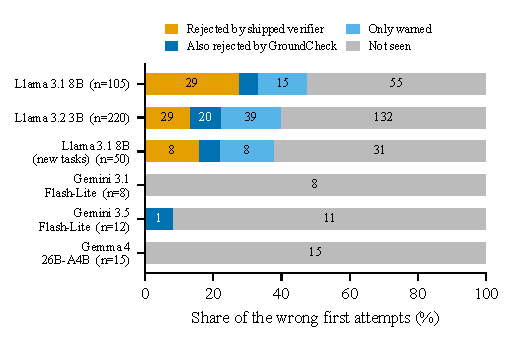
\includegraphics[width=\columnwidth]{figures/fig_e5_taxonomy}
\caption{What verification sees among the formulas each model gets wrong at attempt 1 (final system). Numbers are formulas.}
\label{fig:e5-taxonomy}
\end{figure}

\paragraph{Repair}
\begin{table*}[!t]
\caption{End-to-end execution accuracy (\%) of the production formula agent after up to two repair attempts, by repair strategy, with retrieved context. $\Delta$: percentage points over attempt 1; $p_{\text{Holm}}$: exact McNemar test against plain resampling (same tasks, paired), Holm-adjusted over the four feedback strategies of each model. Models whose first attempts are almost never rejected are omitted: no strategy has anything to repair.}
\label{tab:e5-repair}

\centering\footnotesize
\begin{tabular}{l rrr rrr rrr}
\toprule
& \multicolumn{3}{c}{\textbf{Llama~3.1 8B} (n=360)} & \multicolumn{3}{c}{\textbf{Llama~3.2 3B} (n=360)} & \multicolumn{3}{c}{\textbf{Llama~3.1 8B, new tasks} (n=180)} \\
\cmidrule(lr){2-4}\cmidrule(lr){5-7}\cmidrule(lr){8-10}
\textbf{Condition} & Acc. & $\Delta$ & $p_{\text{Holm}}$ & Acc. & $\Delta$ & $p_{\text{Holm}}$ & Acc. & $\Delta$ & $p_{\text{Holm}}$ \\
\midrule
Attempt 1 (no repair) & 70.8 & -- & -- & 38.9 & -- & -- & 72.2 & -- & -- \\
Resample (no feedback) & 71.1 & +0.3 & -- & 39.2 & +0.3 & -- & 72.8 & +0.6 & -- \\
Generic feedback & 72.2 & +1.4 & .125 & 39.7 & +0.8 & 1.000 & 72.8 & +0.6 & 1.000 \\
Shipped-verifier feedback & 74.2 & +3.3 & .007 & 39.7 & +0.8 & 1.000 & 74.4 & +2.2 & .750 \\
GroundCheck feedback & \textbf{74.4} & +3.6 & .001 & \textbf{40.0} & +1.1 & 1.000 & \textbf{75.0} & +2.8 & .375 \\
GroundCheck + suspicious & \textbf{75.3} & +4.4 & <.001 & \textbf{40.0} & +1.1 & 1.000 & \textbf{76.1} & +3.9 & .125 \\
\bottomrule
\end{tabular}
\end{table*}

Table~\ref{tab:e5-repair} and Figure~\ref{fig:e5} compare feedback strategies from the same first attempt. Asking again without feedback repairs almost nothing (\efASresample\%, $+$\efASresampleD{} points); a generic ``try again'' message gives \efASgeneric\% ($+$\efASgenericD{}); diagnostics from the shipped verifier \efASvonefb\% ($+$\efASvonefbD{}); and \gc{} diagnostics \efASvtwofb\% ($+$\efASvtwofbD{} points, 95\% interval [\efASvtwofbLo, \efASvtwofbHi]; \efASvtwofbFixed{} tasks fixed, none broken), better than resampling (Holm-adjusted $p$ \hmAHolmVtwoRes) and than the generic message ($p$ \hmAHolmVtwoGen). Also repairing on suspicious findings reaches \efASvtwofbplussusp\% ($+$\efASvtwofbplussuspD{}). The feedback of the two verifiers is not distinguishable here ($p$ \hmAHolmVtwoVone; they fix \efASvtwofbFixed{} and \efASvonefbFixed{} tasks), for the reason given above. The ordering is the same with the shipped chunk format (Table~\ref{tab:e5-repair-shipped}). Repair costs about \efAExtravtwofb{} extra model calls per task. The hosted models are absent from Table~\ref{tab:e5-repair} because they rarely give the verifier anything to reject.

\begin{figure}[t]
\centering
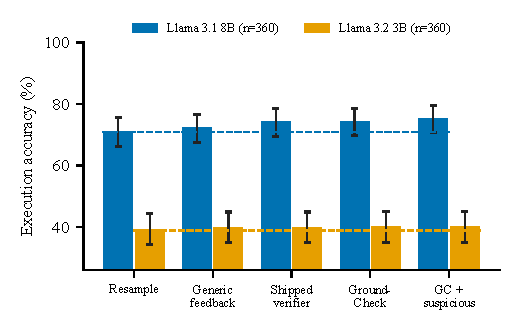
\includegraphics[width=\columnwidth]{figures/fig_e5_repair}
\caption{Execution accuracy after repair (GC: \gc) for the models whose attempts the verifier rejects often enough to compare strategies. Dashed lines: accuracy at attempt 1; error bars: 95\% Wilson intervals.}
\label{fig:e5}
\end{figure}

\paragraph{Run-to-run variation}
\ifdefined\sdASeeds
One sampled trajectory per task could mislead, so we reran the local models on the same tasks with \sdASeeds{} sampling seeds (Table~\ref{tab:e5-seeds}). Accuracy at attempt 1 with retrieved context is \sdARetr\% (SD \sdARetrSD{} points) for \efAName{} and \sdBRetr\% (SD \sdBRetrSD) for \efBName: the seed moves a model's accuracy by about a point, less than the differences between context formats or repair strategies that we interpret. For \efAName{} \gc{} feedback beats plain resampling in \sdASeedsBeat{} of \sdASeeds{} seeds, by \sdADvtwofbresample{} points on average over seeds and tasks (task-clustered 95\% interval [\sdADvtwofbresampleLo, \sdADvtwofbresampleHi]); against the shipped verifier's feedback the difference is \sdADvtwofbvonefb{} points [\sdADvtwofbvonefbLo, \sdADvtwofbvonefbHi]. For \efBName{} \gc{} feedback also beats resampling in \sdBSeedsBeat{} of \sdBSeeds{} seeds, but by only \sdBDvtwofbresample{} points [\sdBDvtwofbresampleLo, \sdBDvtwofbresampleHi]: a small effect that a single run (Table~\ref{tab:e5-repair}) cannot resolve.

\begin{table}
\caption{Run-to-run variation on the 360 main-set tasks: the same tasks rerun with 3 independent sampling seeds. The interval for the repair effect is a paired bootstrap over tasks of each task's outcome averaged over seeds.}
\label{tab:e5-seeds}

\centering\footnotesize
\begin{adjustbox}{max width=\columnwidth}\begin{tabular}{l rr}
\toprule
\textbf{Accuracy, mean (SD) over seeds} & \textbf{\shortstack[r]{Llama~3.1\\8B}} & \textbf{\shortstack[r]{Llama~3.2\\3B}} \\
\midrule
Attempt 1, active sheet only & 72.2 (0.3) & 35.8 (1.5) \\
Attempt 1, retrieved context & 71.4 (0.6) & 39.4 (0.7) \\
Resample (no feedback) & 71.6 (0.4) & 39.7 (0.7) \\
Generic feedback & 73.1 (0.8) & 40.2 (0.6) \\
Shipped-verifier feedback & 74.8 (0.7) & 40.4 (0.9) \\
GroundCheck feedback & 75.6 (1.1) & 40.8 (1.0) \\
GroundCheck + suspicious & 76.2 (0.8) & 41.0 (1.1) \\
\midrule
\gc{} feedback $-$ resample, points [95\% CI] & 4.0 [2.2, 5.9] & 1.1 [0.3, 2.2] \\
\gc{} feedback $-$ shipped feedback, points [95\% CI] & 0.7 [0.1, 1.6] & 0.5 [0.1, 1.0] \\
Seeds in which \gc{} beats resampling & 3 of 3 & 3 of 3 \\
\bottomrule
\end{tabular}\end{adjustbox}
\end{table}

\else
Further sampling seeds were not run for this version.
\fi

\paragraph{Does repair make failures safer?}
Accuracy counts whether the final cell is right and says nothing about what the wrong cells look like. Table~\ref{tab:e5-harm} accounts for every task under three policies. With \efAName, writing the first attempt unchecked leaves \hmAAsIsLoud{} cells that show an error and \hmAAsIsSilent{} that show a plausible wrong value, out of \hmAN. Withholding what \gc{} rejects, without repair, holds back \hmABlockWithheld{} formulas, all of them wrong (\hmAFalseWithheld{} correct formulas withheld), and leaves the silent errors as they were. Repairing with \gc{} feedback (Figure~\ref{fig:e5-fate}) fixes \hmAUnsafeVtwoFixed{} of the \hmAUnsafeN{} rejected attempts, but of the others \hmAUnsafeVtwo{} end as plausible wrong values and \hmAUnsafeVtwoLoud{} still show an error: the \emph{unsafe-repair rate} is \hmAUnsafeVtwoRate\% (shipped feedback: \hmAUnsafeVoneRate\%; resampling: \hmAUnsafeResRate\%, because it rarely changes anything). As a result the silent errors \emph{rise}, from \hmAAsIsSilent{} to \hmARepVtwoSilent, while the visible errors fall from \hmAAsIsLoud{} to \hmARepVtwoLoud. The picture is the same for \efBName{} (silent \hmBAsIsSilent{} to \hmBRepVtwoSilent, unsafe-repair rate \hmBUnsafeVtwoRate\%) and on the held-out tasks (\hmCAsIsSilent{} to \hmCRepVtwoSilent). \ifdefined\sdASeeds It holds across seeds: the unsafe-repair rate of \efAName{} averages \sdAUnsafevtwofb\% over the \sdASeeds{} seeds, ranging from \sdAUnsafevtwofbMin\% to \sdAUnsafevtwofbMax\%.\fi

\begin{table}
\caption{What ends up in the cell, as \% of tasks, under three policies: write the first attempt unchecked; withhold what \gc{} rejects and write the rest (no repair); repair with \gc{} feedback. \emph{Right}: evaluates to the gold value. \emph{Error}: the cell shows an error value. \emph{Silent}: a plausible but wrong value (the failure a user cannot see). \emph{Held}: nothing is written.}
\label{tab:e5-harm}

\centering\footnotesize
\begin{adjustbox}{max width=\columnwidth}\begin{tabular}{l l rrrr}
\toprule
\textbf{Model} & \textbf{Policy} & \textbf{Right} & \textbf{Error} & \textbf{Silent} & \textbf{Held} \\
\midrule
\multirow{3}{*}{Llama~3.1 8B} & Write as is & 70.8 & 18.6 & 10.6 & -- \\
 & Block rejected & 70.8 & 8.9 & 10.6 & 9.7 \\
 & Repair (\gc) & 74.4 & 12.5 & \textbf{13.1} & -- \\
\midrule
\multirow{3}{*}{Llama~3.2 3B} & Write as is & 38.9 & 30.6 & 30.6 & -- \\
 & Block rejected & 38.9 & 16.9 & 30.6 & 13.6 \\
 & Repair (\gc) & 40.0 & 24.2 & \textbf{35.8} & -- \\
\midrule
\multirow{3}{*}{Llama~3.1 8B new tasks} & Write as is & 72.2 & 16.1 & 11.7 & -- \\
 & Block rejected & 72.2 & 10.0 & 11.7 & 6.1 \\
 & Repair (\gc) & 75.0 & 12.2 & \textbf{12.8} & -- \\
\bottomrule
\end{tabular}\end{adjustbox}
\end{table}


Verification-guided repair therefore raises accuracy by turning some visible failures into correct formulas and others into invisible ones: of the visible errors it removes, only part become right. Blocking and showing the diagnostics has no such side effect, and the case for repair rests on how much a user's attention is worth. Since the outcome of a repaired formula is a valid-looking value, we regard an execution check, or showing the computed value next to the request, as the natural next step. An execution check in a scratch cell would catch the cells that show an error (\hmAAsIsLoud{} before repair and \hmARepVtwoLoud{} after, for \efAName) but none of the silent ones, which only the computed value, read against the request, can expose.

\ifdefined\exASame
\emph{Adding an execution check.} The cells that still show an error after repair are loud faults the workbook-state checks did not see. We therefore added a second stage to the pipeline, verify, repair, \emph{execute}: after \gc{} accepts a formula, it is evaluated in the workbook (in the add-on, in a scratch cell) and an error is sent back to the model (Table~\ref{tab:e5-exec}; first attempts regenerated with the same seed reproduced the stored one for \exASame{} of \exATotal{} tasks of \efAName). Of the \exALoudAfter{} cells that still show an error after \gc{} repair, the execution check fixes \exALoudFixed{}, leaves \exALoudStill{} and turns \exALoudToSilent{} into plausible wrong values; overall \exAExecCorrect{} formulas are right against \exAVtwoCorrect{} with repair alone (+\exAGained{}/$-$\exALost{} tasks, $p$ \exAP), and silent errors go from \exAVtwoSilent{} to \exAExecSilent. For \efBName{} (\exBSame{} tasks) the check fixes \exBLoudFixed{} of the \exBLoudAfter{} cells that still show an error after repair and turns \exBLoudToSilent{} into plausible wrong values; silent errors go from \exBVtwoSilent{} to \exBExecSilent. The check removes some visible errors but no silent ones: it cannot see them, and repairing an error can again produce a plausible wrong value, so the number of silent errors does not fall.

\begin{table}
\caption{What ends up in the cell (\% of tasks) when repair is followed by an execution check: after the verifier accepts a formula, the cell is evaluated and an error is sent back to the model. Only tasks whose regenerated first attempt reproduced the stored one are included, so all three policies cover the same tasks.}
\label{tab:e5-exec}

\centering\footnotesize
\begin{adjustbox}{max width=\columnwidth}\begin{tabular}{l l rrr}
\toprule
\textbf{Model} & \textbf{Policy} & \textbf{Right} & \textbf{Error} & \textbf{Silent} \\
\midrule
\multirow{3}{*}{Llama~3.1 8B} & Write as is & 75.2 & 16.2 & 8.6 \\
 & Repair (\gc) & 78.3 & 10.4 & 11.3 \\
 & Repair + execution & 80.1 & 7.6 & \textbf{12.2} \\
\midrule
\multirow{3}{*}{Llama~3.2 3B} & Write as is & 45.1 & 26.3 & 28.6 \\
 & Repair (\gc) & 46.5 & 19.2 & 34.3 \\
 & Repair + execution & 47.8 & 15.2 & \textbf{37.0} \\
\bottomrule
\end{tabular}\end{adjustbox}
\end{table}

\fi

\begin{figure}[t]
\centering
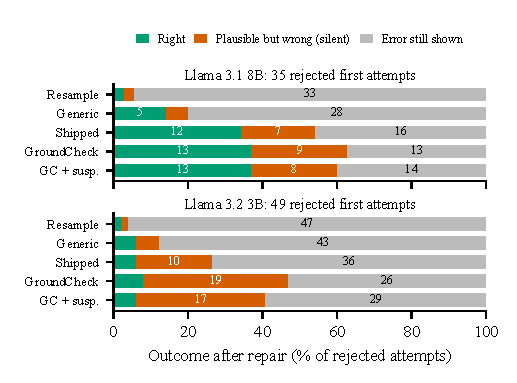
\includegraphics[width=\columnwidth]{figures/fig_e5_repair_fate}
\caption{Outcome of repair for the attempts \gc{} rejected, by strategy: right, a plausible but wrong value (silent), or an error still shown. Numbers are attempts; segments under 9\% are unlabelled.}
\label{fig:e5-fate}
\end{figure}

\paragraph{Where the models fail}
Accuracy by task template (Figure~\ref{fig:e5-templates}, Appendix~\ref{app:results}) shows the pattern behind the totals. The local models fail on the same few templates: \efATemplateZero{} of the \efNTemplates{} templates (the cross-sheet lookup) is solved on fewer than one task in twenty by \efAName{} and \efBTemplateZero{} by \efBName, whereas the hosted models' lowest template accuracies are \efDTemplateMin\%, \efETemplateMin\% and \efFTemplateMin\%. Requests that paraphrase the column names instead of quoting the headers are harder for the two local models on the main set (\efAFormS\% against \efAFormH\% for \efAName, \efBFormS\% against \efBFormH\% for \efBName) but not on the held-out set (\efCFormS\% against \efCFormH\%); we do not read more into it.
\ifdefined\efBN
\paragraph{A smaller model}
\efBName{} is correct at attempt 1 in \efBfinal\% of tasks (\efBflat\% with the active sheet only, $p$ \efBTestfinalvsflatP). It makes more of the errors that only \gc{} sees: the verifier rejects \efBCaughtTwo{} of its \efBWrong{} wrong first attempts, against \efBCaughtOne{} for the shipped one. But it makes little use of the feedback. In the main run repair raises accuracy by \efBSvtwofbD{} points ($p$ \efBSvtwofbP{} against attempt 1; \efBSvtwofbFixed{} tasks fixed), which no strategy distinguishes from resampling (Table~\ref{tab:e5-repair}); only the average over seeds resolves a gain of about a point. Feedback needs a model able to act on it. As an acceptance gate the verifier still separates the two groups: formulas it accepts are correct \efBGateAcc\% of the time and those it rejects \efBGateRej\%.
\fi
\paragraph{Hosted models}
The hosted models are right at attempt 1 on \efDfinal\%, \efEfinal\% and \efFfinal\% of their tasks (\efDflat\%, \efEflat\% and \efFflat\% with the active sheet only), so they leave the verifier almost nothing to do: they make few errors, most of them silent (\efDSilent{} of \efDWrong, \efESilent{} of \efEWrong, \efFSilent{} of \efFWrong), and no repair strategy has anything to repair. For models this accurate on these tasks the verifier is a safety net that costs nothing, and the benefit of the add-on comes from the context it supplies. This is no verdict on the value of verification for stronger models on harder work: \sheetfault{} tasks are single formulas over one or two tables, while workflow-level benchmarks find frontier agents failing far more often~\cite{zhu2026spreadsheetbench2}. The two Gemini runs were capped by the free tier's daily quota, so each covers the first tasks of a fixed hash order (\efDN{} and \efEN{} of the 360), a subset chosen without regard to difficulty; the Gemma run covers \efFN{}.


\ifdefined\sixN
\subsection{Why not ask the model?}
\label{sec:e6}
\begin{table}
\caption{A language-model critic (same model and context as the generator) versus the deterministic verifier on a stratified sample of \sheetfault{}; recall in \% when blocking only on rejection.}
\label{tab:e6}

\centering\footnotesize
\begin{adjustbox}{max width=\columnwidth}\begin{tabular}{l r rrr}
\toprule
\textbf{Fault group} & n & Critic & \gc & Either \\
\midrule
Structural & 25 & 44 & 100 & 100 \\
Symbols & 37 & 65 & 92 & 92 \\
Shape & 15 & 87 & 100 & 100 \\
Grounding & 14 & 29 & 0 & 29 \\
Circularity & 33 & 61 & 100 & 100 \\
Semantic & 16 & 38 & 19 & 38 \\
\midrule
All faults & 140 & 55.7 & 78.6 & 83.6 \\
Clean formulas rejected (FPR) & 161 & 21.1 & 0.0 & 21.1 \\
\bottomrule
\end{tabular}\end{adjustbox}
\end{table}

A critic given the same model and context (\sixN{} sampled instances, \sixFaults{} faulty; Table~\ref{tab:e6}) rejects \sixCriticR\% of faults and \sixCriticFPR\% of clean formulas (F1 \sixCriticF), against \sixVerR\% and \sixVerFPR\% for the verifier on the same sample (F1 \sixVerF). It catches only \sixCriticStructural\% of the structural faults, which a parser sees at no cost, and \sixCriticCircular\% of circular references (verifier: \sixVerCircular\%). It does catch \sixCriticOnlyCaught{} faults the verifier does not (chiefly \sixCriticOnlyWhere), against \sixVerOnlyCaught{} the other way round (the verifier flags the grounding cases but by policy does not reject them); combining the two raises recall to \sixEitherR\% but false positives to \sixEitherFPR\%. Asking the model is a poor replacement for a parser and at best a complement where the workbook cannot adjudicate.
\fi

\subsection{Context retrieval under a token budget}
\label{sec:e2}
When the whole workbook fits the budget, retrieval is moot: at \eTwoZeroFull{} tokens (10 tables) every ranking method, even random, retrieves all gold tables at a 1{,}500-token budget (\eTwoZeroComplete\% for the ranker). It becomes informative as workbooks grow. At \eTwoTables{} tables (\eTwoFull{} tokens, \eTwoReq{} requests, budget 1{,}500, \eTwoReduction\% fewer tokens than sending everything) the ranker keeps all gold tables in \eTwoRankerComplete\% of requests against \eTwoBmComplete\% for BM25 and \eTwoRandComplete\% for random, and the shipped agent's active-sheet context holds none (Table~\ref{tab:e2} and Figure~\ref{fig:e2}, Appendix~\ref{app:results}); at a 500-token budget the figures are \eTwoRankerCompleteSmall\% and \eTwoBmCompleteSmall\%. Adding column letters made every chunk longer, so the same budget holds fewer tables: the cost of the fix in Section~\ref{sec:e5}. Figure~\ref{fig:e2-scale} shows the same budget as the workbook grows: the ranker and BM25 are equal while everything fits, the gap opens as the workbook outgrows the budget, and the active-sheet context never holds the gold tables.

\begin{figure}[t]
\centering
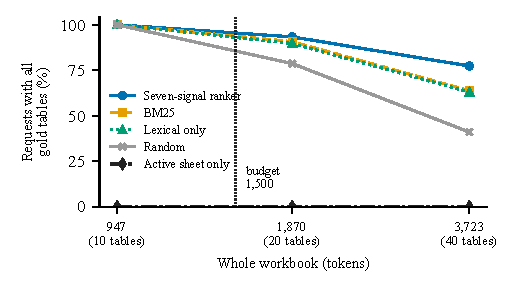
\includegraphics[width=\columnwidth]{figures/fig_e2_scale}
\caption{Share of requests whose prompt contains every gold table at a 1{,}500-token budget, as the workbook grows (10, 20 and 40 tables).}
\label{fig:e2-scale}
\end{figure}

\begin{table}
\caption{Gold-complete rate (\%) by request type at 40 tables, budget 1500. A: aggregate; B: lookup; C: ``change \emph{this} formula\textquotedblright{}. H: names the column; S: paraphrase only.}
\label{tab:e2-type}

\centering\footnotesize
\begin{adjustbox}{max width=\columnwidth}\begin{tabular}{l rrrrr}
\toprule
\textbf{Method} & A-H & A-S & B-H & B-S & C \\
\midrule
Ranker & 100 & 30 & 100 & 57 & 100 \\
Lexical only & 100 & 30 & 100 & 57 & 28 \\
Graph signals only & 28 & 28 & 50 & 50 & 100 \\
Ranker $-$ graph & 100 & 30 & 100 & 57 & 10 \\
BM25 & 100 & 33 & 100 & 57 & 28 \\
Random & 28 & 45 & 47 & 48 & 37 \\
\bottomrule
\end{tabular}\end{adjustbox}
\end{table}

Lexical overlap solves requests that name the data and graph signals those that do not (Table~\ref{tab:e2-type}): for ``change this to an average'' the ranker finds the table in \eTwoRankerC\% of requests, BM25 in \eTwoBmC\%, and the ranker without its two graph signals in \eTwoNoGraphC\%. The graph signals are redundant with each other, so removing one changes nothing. The structural signals add nothing on this benchmark. Paraphrase is the weak spot: with no shared word, \eTwoRankerAS\% (aggregates) and \eTwoRankerBS\% (lookups) of requests are gold-complete.

\subsection{Cost, and the fetch boundary (secondary)}
\label{sec:e3}
Analysis costs about 11 \code{SpreadsheetApp} calls plus \eScaleCallsPerSheet{} per sheet, independent of rows; verifying one formula costs \eScaleVerifyVone{} calls in the shipped verifier and \eScaleVerifyVtwo{} in \gc{} (a constant increase for column profiles, plus \eScaleVerifyPerSheet{} per sheet); CPU time stays below \eScaleMaxAnalyzeMs{} ms for analysis and \eScaleMaxVerifyMs{} ms for verification even at 2{,}000 formulas (Table~\ref{tab:e3} and Figure~\ref{fig:e3-cost}, Appendix~\ref{app:results}; Apps Script latency itself is not measured), negligible next to a model call.

The URL validator is a secondary result, included because the same check-before-acting idea guards the add-on's one outbound channel. On the corpus of Table~\ref{tab:ssrf} (Appendix~\ref{app:results}), the shipped URL filter blocks \ssrfvoneRecall\% of \ssrfBlock{} must-block URLs (\ssrfvoneBypass{} bypasses, including every decimal, hexadecimal and octal encoding of loopback and private addresses, \code{127.1}, and every internal-only name) and wrongly blocks \ssrfvoneFalseBlock\% of \ssrfAllow{} benign URLs, because it matches substrings of the whole URL (\code{https://210.1.2.3/} is rejected for containing \code{10.1.2.3}). The parse-and-classify validator blocks \ssrfvtwoRecall\% (95\% interval lower bound \ssrfvtwoCILo\%) with \ssrfvtwoFalseBlock\% false blocks. The corpus was built by us from known bypass classes, so it measures coverage, not adversarial robustness; one bypass (a backslash before \code{@}) was found by the first run and fixed.

\section{Discussion}
\label{sec:discussion}

\paragraph{The verifier needed verifying}
Replacing regular expressions with a parser and range-aware dependency analysis immediately broke the add-on's own test suite: nearly every fixture inserted \code{=SUM(B2:B3)} into B2, a circular reference the shipped verifier never noticed. The real-world corpus then found two defects in our new verifier, and one in our own corpus extraction, in a single pass, and a confirmation set scored with the verifier frozen found a further gap, deleted references, that the benchmark could not have shown because we had not thought of it. A deterministic check is easy to believe; one that is wrong in either direction silently degrades the agent it guards, so a labelled fault benchmark, a clean-negative corpus and real formulas should accompany any such component, and the real formulas should be scored in a way that cannot be tuned after the fact.

\paragraph{What deterministic checks buy, and where they stop}
On the benchmark nearly all loud faults and most silent ones are stopped or flagged, the contribution concentrated in a few cheap layers; on real formulas the two verifiers reject about the same share, and what differs is the kind of fault. End to end the picture is more modest: a few points for an 8B model, about one for a 3B model that can barely act on feedback, and little advantage over the shipped verifier because these models mostly make errors both catch. The hosted models make almost no errors the workbook can see, so the checks are idle and the context decides accuracy; the checks matter for the models that need them, and cost the others nothing. What remains is what the workbook cannot adjudicate (Section~\ref{sec:levels}): a valid formula over the wrong data.

\paragraph{Repair trades visible for invisible failures}
The most useful result may be the least flattering. Verification-guided repair raises accuracy, yet it also raises the number of plausible-but-wrong values written into the sheet, because a formula repaired into validity is no more likely to be right than the one it replaced, and a wrong value that looks right is the failure a user cannot see. In our runs \hmAUnsafeVtwoRate\% (\efAName) to \hmBUnsafeVtwoRate\% (\efBName) of the rejected attempts end that way. Whether that trade is worth it depends on what a visible error costs: a user sees \code{\#REF!} at once, but may never see a wrong total. A design that holds the rejected formula, shows the diagnostics and lets the user decide has no such side effect; one that repairs should follow with an execution check and show the computed value next to the request. The add-on's approval step, dry run and undo address the problem procedurally.

\paragraph{Policy, latent faults and prompts}
Which findings block is a policy: we block only what the workbook proves impossible or a near-miss of something real, and demote plausible-but-probably-wrong findings to \emph{suspicious}, whose repair is worth a further point (Table~\ref{tab:e5-repair}). Value-based checks, including the execution accuracy used by most benchmarks, cannot see about one percent of real formulas (\rwcFGhostOkMasked{} of \rwcFFormulas{} in the confirmation set) that reference a missing sheet behind \code{IFERROR}. And prompts anchor: one of three worked examples in the add-on's prompt uses a sheet called \code{Sheet2}, and on lookup tasks \efAName{} wrote \code{Sheet2!\dots} in \efALkSheetTwo{} of \efALkN{} first attempts although the request names the real sheet. The symbols layer rejects every such formula and its hint lists the real sheets; repair lifts lookup accuracy from \efALkBase\% to \efALkvtwofb\% (resampling: \efALkresample\%). A verifier is no excuse for a careless prompt, but it turns a systematic prompt defect from a silent wrong answer into a one-step repair.

\paragraph{Evaluating a verifier you wrote}
A benchmark written alongside the component it tests measures coverage of the authors' idea of faults. We used four countermeasures, none sufficient alone: labels from an independent engine, real formulas, a confirmation set scored once with a frozen verifier, and a harness for checking the labels in Google Sheets itself (Appendix~\ref{app:gsheets}). The real-formula result was sobering, and it is the one that exposed the gap.

\section{Limitations and Threats to Validity}
\label{sec:limitations}

\paragraph{The benchmark is synthetic and co-designed with the verifier}
\sheetfault{} workbooks, request templates and fault operators were written by us alongside \gc. Near-perfect recall on a class therefore shows that the class is \emph{covered}, not that the verifier generalizes to faults we did not think of, and the clean negatives are valid by construction. Independent evidence comes from the real-formula sets, which measure rejection rates without ground truth, and from the end-to-end study, where the language models produce their own faults; the confirmation run showed that the benchmark missed a class of real defects. The benchmark has no dates, arrays, text manipulation or formatting, and its natural-language requests are templated. Its workbook-clustered intervals are narrow because one generator produces every workbook; they measure sampling noise, not how representative the workbooks are.

\paragraph{Labels come from HyperFormula, not from Google Sheets}
HyperFormula follows Excel semantics and lacks some Sheets functions (\code{QUERY}, \code{AVERAGEIFS}, \dots). Where products differ, as with unequal \code{SUMIF} ranges, the label may differ from what Google Sheets would do; the \code{QUERY} class is labelled by construction. The system is presented for Google Sheets, so this is a real threat. The repository contains a harness that evaluates a stratified sample of benchmark cases in an actual Google Sheet and compares the answers (Appendix~\ref{app:gsheets}). \ifdefined\gsN Its result is reported there.\else The harness was tested against a mock but has not been run in Google Sheets for this version, so all labels here are HyperFormula labels.\fi{} Scalar-valued tasks only.

\paragraph{No independent human labels for real formulas}
The released Sheetpedia files carry no cached results, so there are no labels: we report rejection rates and use an engine's evaluation of the original formula as supporting evidence, not as ground truth. A rejected formula that the engine evaluates without error may still be broken (a missing sheet behind \code{IFERROR}) or fine (an exempted pattern), and an accepted formula may be wrong in a way neither verifier sees. We therefore claim no precision or recall on real formulas. \ifdefined\annN Independent annotation is reported in Appendix~\ref{app:annotation}.\else A protocol and tooling for blind annotation by two annotators are part of the repository (Appendix~\ref{app:annotation}); the annotation itself is not part of this version.\fi{} A large group of rejections (references to missing sheets) may partly reflect sheets removed by the dataset's PII processing, and some formulas were blanked by it. The corpus is Excel-flavoured and excludes structured and external references.

\paragraph{Verifier changes made after seeing data}
Two changes followed the real-formula sets. One exempted \code{COUNTA}, \code{COUNTBLANK} and \code{ISBLANK} after the first held-out run, and we report the first-pass figure as the held-out result. The other added two rules after the first confirmation run; the figures of that set for the extended verifier are post hoc, and the confirmatory evidence for the extended verifier is the second confirmation set \ifdefined\rwcGFormulas (\rwcGFormulas{} formulas)\else (not yet scored in this version)\fi. Each set measures one draw of workbooks, and rejections are concentrated in few of them.

\paragraph{Few models, simple tasks}
The end-to-end study uses two 4-bit quantized open models served locally, two hosted Gemini models and one hosted open-weight model (Gemma~4); we ran no model from OpenAI or Anthropic, and the hosted runs were limited by a free tier's quotas (the larger Gemini Flash models allow only about twenty requests a day, so we could not use them) and use one sampling trajectory per task. The tasks are single formulas over one or two tables, and the hosted models solve nearly all of them, which leaves the verifier idle; harder, multi-step work, where frontier agents fail far more often~\cite{zhu2026spreadsheetbench2}, is not covered, so the absolute accuracies and the value of repair should not be read as transferable. The local models were run with three seeds; the seed moves accuracy by about a point. The fix to the retrieved table chunks (column letters and the data-row span) was motivated by the first pass over the main task set, so its effect on that set is a post hoc comparison; we therefore confirm it on a fresh held-out set of workbooks. The repair $p$-values are Holm-adjusted within each model but not across models. Model identifiers and the versions the API reported are stored with the results; a hosted model may change or be withdrawn after our runs, and its sampling is not exactly reproducible.

\paragraph{Not measured}
There is no user study, so we do not know how users respond to warnings or repaired formulas, or whether the unsafe repairs we count would have been noticed. Timings are Node CPU time and \code{SpreadsheetApp} call counts, not Apps Script latency. We do not evaluate the planner's approval step, intent routing, or undo and rollback. The function whitelist is the English documentation list and locale-specific argument separators are only partly handled. The SSRF corpus is a secondary result, built from known bypass classes by the authors; it measures coverage, not adversarial robustness, and DNS rebinding is out of scope for a static check.

\section{Ethics and Reproducibility}
\paragraph{Ethics}
We use Sheetpedia, released under CC BY-SA~4.0 after PII processing; we do not redistribute any workbook and report aggregates and generic formula fragments only. Two of the language models are open-weight and ran locally on a consumer GPU; the hosted models received only synthetic workbooks. No user data were collected. The URL corpus consists of standard, publicly documented encodings of private addresses and is intended for defence. The main risk of the system is false assurance: a formula that passes verification may still answer the wrong question, and the add-on sends sheet content (headers, sample values, formulas) to a hosted model when used with one, which users should weigh for sensitive data.

\paragraph{Reproducibility}
Every generator is seeded and every table and number in this paper is produced from result files by a script. The repository accompanying this paper contains the add-on, the 163-test suite, the evaluation harness, the raw trajectories and the scripts that regenerate all tables and figures, and a script that audits the built paper (references, citations, floats, macros). Software versions: Node.js 24.14, HyperFormula 3.4.0, Ollama with \code{llama3.1:8b} (digest \code{46e0c10c039e}) and \code{llama3.2:3b} (digest \code{a80c4f17acd5}); the hosted models are \code{gemini-3.1-flash-lite}, \code{gemini-3.5-flash-lite} and \code{gemma-4-26b-a4b-it}, accessed on 2 October 2026, with the version string of every response stored. The shipped verifier compared throughout is commit \code{44a3f4f}. The Sheetpedia sets are drawn with a fixed seed from three disjoint parts of the release archive by the extraction script, and the verifier that scored the confirmation sets is identified by the SHA-256 hashes recorded before the data were fetched.


\bibliographystyle{IEEEtran}
\bibliography{refs}

\appendices
% In the appendix, single-column tables may be set where they occur instead of being queued to column tops.
\makeatletter\renewcommand{\fps@table}{!htb}\makeatother

\section{Benchmark details}
\label{app:bench}

\paragraph{Fault operators}
Table~\ref{tab:ops} lists the operators. Each is applied to a gold formula; the result is kept as a fault only if the independent engine returns an error or a different value. Circular classes are generated at the position where users make them: the totals row under a numeric column, so the target cell lies inside the used column span. The \code{QUERY} class is generated from scratch and labelled by construction.

\begin{table}[t]
\caption{Fault operators and semantics-preserving variants used by \sheetfault.}
\label{tab:ops}
\centering\footnotesize
\begin{tabular}{>{\raggedright\arraybackslash}p{1.35cm} >{\raggedright\arraybackslash}p{2.75cm} >{\raggedright\arraybackslash}p{4.0cm}}
\toprule
\textbf{Group} & \textbf{Class} & \textbf{Operator} \\
\midrule
Structural & unbalanced parenthesis / quote & delete the final \code{)} / one \code{"} \\
 & missing \code{=} & drop the leading \code{=} \\
 & injection & append \code{+DDE("cmd|...")} or use a \code{HYPERLINK} to a \code{javascript:} URL \\
Symbols & hallucinated function & rename to a plausible invented name (\code{SUMIFF}, \code{COUNTWHERE}, \code{MEAN}, \code{NTHLARGEST}, \dots) \\
 & non-existent sheet & singular/plural variant, \code{Sheet2}, \code{Data}, \code{<name>\_old}, or prefix an own-sheet range with a missing sheet \\
 & column beyond data & move a range to a column 1--6 past the last used column \\
 & header used as name & replace a range by its column's header text (\code{=SUM(Revenue)}) \\
 & \code{QUERY} column OOB & select a column letter beyond the range's width \\
Shape & lookup index too large & \code{VLOOKUP} index = number of lookup columns + 3 \\
 & range size mismatch & shorten the last range of a multi-range function by 5--15 rows \\
Grounding & criterion absent & alter a string criterion (\code{"East"} $\to$ \code{"Easts"}, \code{"Northeast"}) \\
 & aggregate over text & replace the aggregated numeric range by a categorical column \\
Circularity & self reference & add the target cell to the formula \\
 & range / column contains self & totals-row range \code{F2:F81} or whole column \code{F:F} in \code{F81} \\
 & cycle via cell / range & the formula reads a helper cell whose formula reads the target cell / a range containing it \\
Semantic & wrong numeric column & swap one numeric range for another numeric column \\
 & wrong function & \code{SUM}$\leftrightarrow$\code{AVERAGE}, \code{MAX}$\leftrightarrow$\code{MIN}, \code{SUMIF}$\leftrightarrow$\code{AVERAGEIF}, \dots \\
\midrule
Benign variants & (negatives) & rows of headroom; absolute references; whole-column references; lowercase function names; extra spacing; own-sheet prefix; \code{IFERROR} wrapper; named range \\
\bottomrule
\end{tabular}
\end{table}

\paragraph{Task templates}
Fourteen templates: aggregate (\code{SUM/AVERAGE/MAX/MIN}), record count, conditional sum, conditional count, conditional average, two-condition \code{SUMIFS}/\code{COUNTIFS}, cross-sheet \code{VLOOKUP}, share of total, count above a threshold, \code{MAXIFS}, \code{SUMPRODUCT}, rounded average, $k$-th largest, and \code{INDEX/MATCH} for the row with the largest value. Each has an exact-header surface form (\emph{Sum Revenue where Region is East.}) and a paraphrase form (\emph{What is the total sales for the East territory?}) whose column mentions share no token with the headers.

\begin{table}
\caption{Share of clean formulas rejected or flagged, by class (\%). Every class is valid by construction or confirmed equivalent to the gold formula by the engine; custom functions cannot be checked and are only warned about.}
\label{tab:e1-clean}

\centering\footnotesize
\begin{adjustbox}{max width=\columnwidth}\begin{tabular}{l r rr rr}
\toprule
& & \multicolumn{2}{c}{\textbf{Shipped (v1)}} & \multicolumn{2}{c}{\textbf{\gc}} \\
\cmidrule(lr){3-4}\cmidrule(lr){5-6}
\textbf{Clean class} & n & Rej. & Flag & Rej. & Flag \\
\midrule
Gold formula & 864 & 0.0 & 15.3 & 0.0 & 0.0 \\
Rows of headroom & 396 & 0.0 & 100.0 & 0.0 & 0.0 \\
Absolute references & 783 & 0.0 & 16.9 & 0.0 & 0.0 \\
Whole-column references & 304 & 0.0 & 1.0 & 0.0 & 0.0 \\
Lowercase function names & 864 & 0.0 & 2.4 & 0.0 & 0.0 \\
Extra spacing & 751 & 0.0 & 17.6 & 0.0 & 0.0 \\
Own-sheet prefix & 783 & 0.0 & 16.9 & 0.0 & 0.0 \\
\code{IFERROR} wrapper & 864 & 0.0 & 15.3 & 0.0 & 0.0 \\
Named range & 99 & 0.0 & 19.2 & 0.0 & 0.0 \\
Ordinary totals-row formula & 864 & 0.0 & 0.0 & 0.0 & 0.0 \\
Valid \code{QUERY} & 144 & 0.0 & 0.0 & 0.0 & 0.0 \\
Handwritten valid syntax & 4{,}032 & 0.0 & 8.9 & 0.0 & 0.0 \\
Custom (non-Sheets) function & 144 & 0.0 & 100.0 & 0.0 & 100.0 \\
\bottomrule
\end{tabular}\end{adjustbox}
\end{table}


\section{Verifier details}
\label{app:verifier}

The function list holds 520 names: the 513 functions of the official Sheets list~\cite{googlefunctions} plus seven that exist but are missing from that table. The shipped list held 150 names and omitted 365 of the 513 official functions, including \code{PRODUCT}, \code{AVERAGEIF}, \code{AVERAGEIFS}, \code{MAXIFS}, \code{GEOMEAN} and \code{COUNTUNIQUE}. A function is a hard error only if it is within edit distance 2 of a known name (1 for names shorter than six characters). Arity entries cover about 90 functions; we compared them with the documented syntax and corrected two. The grounding layer reads at most 500 rows per referenced column and judges a column as categorical only if it was read completely or has at most 25 distinct values. Layer switches live in \code{CONFIG.VERIFICATION.LAYERS} and the repair policy in \code{CONFIG.VERIFICATION.REPAIR\_ON\_SUSPICIOUS}.

\section{Prompts}
\label{app:prompts}
The formula agent's system prompt is: \emph{``You are an expert Google Sheets formula engineer. [memory hints] RULES: 1. Output ONLY the raw formula starting with =. No markdown, no backticks, no explanation. 2. Use the spreadsheet context below to scope ranges correctly. 3. If data goes to row N, use that exact row number (not open-ended ranges unless appropriate). 4. Use the column letters and header names from the context. 5. If the user references a previous formula, check the conversation history.''} followed by three worked examples and the context block. After a failed verification the appended user turn has the form:
\begin{quote}\small\ttfamily
Your formula failed verification on attempt 2:\\
Formula: =SUM(Revenue)\\
HARD ERRORS (must fix):\\
\hspace*{1em}$\times$ "Revenue" is not a function, named range or cell reference.\\
CORRECTION HINTS:\\
\hspace*{1em}$\rightarrow$ "Revenue" is a column header (column D). Reference it by cell range, e.g. D2:D80, not by name.
\end{quote}

\section{Additional results}
\label{app:results}

\paragraph{Detection by fault class}
Table~\ref{tab:e1-classes} gives reject/flag recall for every fault class. \gc{} rejects every structural fault, every circular class, and the non-existent-sheet, header-as-name and lookup-index classes; where it only flags (criterion absent from its column, aggregation over a text column) this is the policy of Section~\ref{sec:gc}. The two semantic classes are valid formulas that answer the wrong question; the few hits in the last row coincide with the share of mutants that are loud.

\begin{table}
\caption{Recall per fault class, as reject/flag \%. \emph{Loud}: the independent engine returns an error value (the user would see it); otherwise the wrong formula evaluates silently to a plausible but wrong value. The two semantic classes are valid formulas that answer the wrong question; no verifier that cannot see the user's intent can reject them.}
\label{tab:e1-classes}

\centering\footnotesize
\begin{adjustbox}{max width=\columnwidth}\begin{tabular}{l c r ccc}
\toprule
\textbf{Fault class} & \textbf{Loud} & \textbf{n} & \textbf{Linter} & \textbf{Shipped} & \textbf{\gc} \\
\midrule
\multicolumn{6}{l}{\emph{Structural}} \\
~~Unbalanced parenthesis & yes &864 & 100/100 & 100/100 & \textbf{100/100} \\
~~Unbalanced quote & yes &581 & 100/100 & 100/100 & \textbf{100/100} \\
~~Missing \texttt{=} & no &864 & 100/100 & 100/100 & \textbf{100/100} \\
~~Injection (DDE/JS) & 54\% &864 & 54/54 & 100/100 & \textbf{100/100} \\
\addlinespace[2pt]
\multicolumn{6}{l}{\emph{Symbols}} \\
~~Hallucinated function & yes &864 & 100/100 & 0/100 & \textbf{64/100} \\
~~Non-existent sheet & yes &860 & 0/0 & 100/100 & \textbf{100/100} \\
~~Column beyond data & 43\% &772 & 0/0 & 0/100 & \textbf{97/97} \\
~~Header used as name & yes &783 & 0/0 & 0/17 & \textbf{100/100} \\
~~QUERY column out of range & yes &144 & 0/0 & 100/100 & \textbf{100/100} \\
\addlinespace[2pt]
\multicolumn{6}{l}{\emph{Shape}} \\
~~VLOOKUP index too large & yes &81 & 0/0 & 0/0 & \textbf{100/100} \\
~~Range size mismatch & yes &387 & 0/0 & 0/33 & \textbf{100/100} \\
\addlinespace[2pt]
\multicolumn{6}{l}{\emph{Grounding}} \\
~~Criterion absent from column & 30\% &505 & 0/0 & 0/23 & \textbf{0/100} \\
~~Aggregate over text column & 30\% &443 & 0/0 & 0/28 & \textbf{0/100} \\
\addlinespace[2pt]
\multicolumn{6}{l}{\emph{Circularity}} \\
~~Self reference & yes &864 & 0/0 & 100/100 & \textbf{100/100} \\
~~Range contains own cell & yes &864 & 0/0 & 0/100 & \textbf{100/100} \\
~~Whole column contains own cell & yes &864 & 0/0 & 0/0 & \textbf{100/100} \\
~~Cycle via other cell & yes &864 & 0/0 & 100/100 & \textbf{100/100} \\
~~Cycle via other range & yes &864 & 0/0 & 0/0 & \textbf{100/100} \\
\addlinespace[2pt]
\multicolumn{6}{l}{\emph{Semantic (undetectable by design)}} \\
~~Wrong numeric column & no &617 & 0/0 & 0/20 & \textbf{0/0} \\
~~Wrong aggregation function & 9\% &407 & 0/0 & 0/52 & \textbf{9/9} \\
\bottomrule
\end{tabular}\end{adjustbox}
\end{table}


\paragraph{Real-world rejections}
Table~\ref{tab:e1b} divides the \rwRejTotal{} rejections of the held-out sample by reason, and Table~\ref{tab:e1b-fresh} the \rwcFRejected{} of the confirmation set. The independent engine returns an error for \rwRejEngineErr{} and \rwcFEngineConfirmed{} of them; \rwcTEmpty{} and \rwcFEmpty{} of these are formulas the dataset's PII pass blanked to \code{=}, so without them the engine confirms \rwcTEngineConfirmedReal{} of \rwcTRealRejected{} and \rwcFEngineConfirmedReal{} of \rwcFRealRejected{}. Of the ghost-sheet rejections for which the engine returns a value (\rwGhostOk{} and \rwcFGhostOk{}), \rwGhostOkMasked{} and \rwcFGhostOkMasked{} sit under an \code{IFERROR} wrapper that turns the missing sheet into a plausible fallback, which is the failure the verifier is meant to surface. In the held-out set the ranges beyond the used columns are mostly \code{COUNTA} on empty cells, which we exempted after seeing them; the frozen verifier of the confirmation set contains that exemption, and the \rwcFCatcol{} rejections of that kind that remain all produce an engine error. The unknown function names are near misses such as \code{SORTBY} and \code{ACONCAT}, which are not Sheets functions, and add-in stubs such as \code{\_FV}, which are rejected as a near miss of \code{FV}: a false positive of the rule that a near miss is a typo. The argument mismatches are \code{SUMIF} with unequal ranges, where spreadsheet products differ.

\begin{table}
\caption{What GroundCheck rejects among 5{,}184 real-world formulas in the held-out Sheetpedia sample (8.6\% rejected). \textquotedblleft{}Engine\textquotedblright{} is HyperFormula evaluating the original formula in its workbook. No cached results exist in the release, so there are no ground-truth labels; rejections are adjudicated by category (Appendix~\ref{app:results}).}
\label{tab:e1b}

\centering\footnotesize
\begin{adjustbox}{max width=\columnwidth}\begin{tabular}{l r r r}
\toprule
\textbf{Rejection reason (\gc)} & \textbf{n} & \textbf{Engine error} & \textbf{Engine ok} \\
\midrule
Sheet absent from workbook & 371 & 319 & 52 \\
Range beyond used columns & 14 & 2 & 12 \\
Empty formula (\texttt{=}) & 33 & 33 & 0 \\
Syntax error & 3 & 3 & 0 \\
Unresolved bare name & 1 & 1 & 0 \\
Unknown function name & 21 & 13 & 8 \\
Argument / range mismatch & 2 & 2 & 0 \\
\midrule
\textbf{Total rejected} & 445 & 373 & 72 \\
\bottomrule
\end{tabular}\end{adjustbox}
\end{table}


\begin{table}
\caption{What GroundCheck rejects among 5{,}537 real-world formulas of the confirmation set, scored once with the frozen verifier (10.4\% rejected). \textquotedblleft{}Engine\textquotedblright{} is HyperFormula evaluating the original formula in its workbook.}
\label{tab:e1b-fresh}

\centering\footnotesize
\begin{adjustbox}{max width=\columnwidth}\begin{tabular}{l r r r}
\toprule
\textbf{Rejection reason (\gc)} & \textbf{n} & \textbf{Engine error} & \textbf{Engine ok} \\
\midrule
Sheet absent from workbook & 355 & 201 & 154 \\
Circular reference & 84 & 84 & 0 \\
Range beyond used columns & 18 & 18 & 0 \\
Empty formula (\texttt{=}) & 107 & 107 & 0 \\
Syntax error & 1 & 1 & 0 \\
Unresolved bare name & 2 & 2 & 0 \\
Unknown function name & 4 & 4 & 0 \\
Argument / range mismatch & 3 & 3 & 0 \\
Other & 2 & 2 & 0 \\
\midrule
\textbf{Total rejected} & 576 & 422 & 154 \\
\bottomrule
\end{tabular}\end{adjustbox}
\end{table}


\paragraph{Cost}
Table~\ref{tab:e3} reports the cost of workbook analysis and of verifying one formula. Analysis makes a fixed number of \code{SpreadsheetApp} calls per sheet and its CPU time grows with the number of formulas but stays far below the latency of a model call. Verification grows linearly with the number of sheets for both verifiers; \gc{} adds a constant 19 calls over the shipped verifier for column profiles.

\begin{table}
\caption{Cost of workbook analysis (CPU ms in Node; SpreadsheetApp calls) and SpreadsheetApp calls per formula verification, as workbooks grow.}
\label{tab:e3}

\centering\footnotesize
\begin{adjustbox}{max width=\columnwidth}\begin{tabular}{rrr rr rr}
\toprule
& & & \multicolumn{2}{c}{\textbf{Analyze}} & \multicolumn{2}{c}{\textbf{Verify} (calls)} \\
\cmidrule(lr){4-5}\cmidrule(lr){6-7}
\textbf{Rows} & \textbf{Sheets} & \textbf{Fml} & ms & calls & v1 & v2 \\
\midrule
100 & 3 & 0 & 1.0 & 35 & 12 & 31 \\
500 & 3 & 0 & 3.2 & 35 & 12 & 31 \\
1{,}000 & 3 & 0 & 5.5 & 35 & 12 & 31 \\
2{,}000 & 3 & 0 & 11.4 & 35 & 12 & 31 \\
500 & 3 & 500 & 5.6 & 35 & 12 & 31 \\
2{,}000 & 3 & 2{,}000 & 20.9 & 35 & 12 & 31 \\
500 & 10 & 100 & 6.2 & 91 & 33 & 52 \\
500 & 20 & 100 & 10.9 & 171 & 63 & 82 \\
500 & 40 & 100 & 15.4 & 331 & 123 & 142 \\
\bottomrule
\end{tabular}\end{adjustbox}
\end{table}


\begin{figure}[!t]
\centering
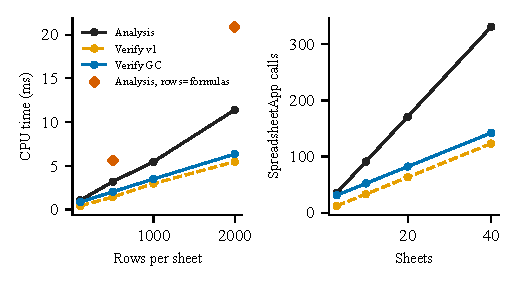
\includegraphics[width=\columnwidth]{figures/fig_e3_cost}
\caption{Cost of workbook analysis and of verifying one formula. Left: CPU time against rows per sheet (three sheets; diamonds: as many formulas as rows). Right: \code{SpreadsheetApp} calls against the number of sheets (500 rows per sheet). The data are those of Table~\ref{tab:e3}.}
\label{fig:e3-cost}
\end{figure}

\paragraph{SSRF corpus}
Table~\ref{tab:ssrf} lists the \ssrfBlock{} must-block and \ssrfAllow{} must-allow URLs by category. The shipped substring filter misses every decimal, hexadecimal, octal and otherwise encoded form of loopback and private addresses and every internal-only name, catches few IPv6-mapped and link-local addresses, and over-blocks benign URLs that contain a private-looking substring; the parse-and-classify validator is correct on all categories.

\begin{table}
\caption{SSRF corpus: URLs handled correctly (blocked if $\ast$, allowed otherwise) by the shipped substring filter (v1) and the parse-and-classify validator (v2).}
\label{tab:ssrf}

\centering\footnotesize
\begin{adjustbox}{max width=\columnwidth}\begin{tabular}{l r rr}
\toprule
\textbf{Category} & \textbf{n} & \textbf{v1} & \textbf{v2} \\
\midrule
$\ast$ loopback (dotted) & 6 & 2 & \textbf{6} \\
$\ast$ loopback (decimal/hex/octal) & 8 & 0 & \textbf{8} \\
$\ast$ loopback (IPv6) & 7 & 3 & \textbf{7} \\
$\ast$ unspecified & 4 & 3 & \textbf{4} \\
$\ast$ localhost names & 5 & 5 & \textbf{5} \\
$\ast$ private v4 (dotted) & 7 & 7 & \textbf{7} \\
$\ast$ private v4 (encoded) & 7 & 0 & \textbf{7} \\
$\ast$ link-local / metadata & 12 & 4 & \textbf{12} \\
$\ast$ IPv6-mapped / translated private & 6 & 2 & \textbf{6} \\
$\ast$ userinfo / authority tricks & 6 & 6 & \textbf{6} \\
$\ast$ wildcard-DNS names for private IPs & 6 & 3 & \textbf{6} \\
$\ast$ internal-only names & 6 & 0 & \textbf{6} \\
$\ast$ non-http schemes & 6 & 6 & \textbf{6} \\
$\ast$ unicode / formatting & 6 & 3 & \textbf{6} \\
public hosts & 8 & 8 & \textbf{8} \\
public IPs & 5 & 5 & \textbf{5} \\
boundary public addresses & 12 & 12 & \textbf{12} \\
public IPs with private-looking digits & 7 & 4 & \textbf{7} \\
benign URLs with suspicious substrings & 12 & 4 & \textbf{12} \\
IDN / unusual but public & 4 & 4 & \textbf{4} \\
\bottomrule
\end{tabular}\end{adjustbox}
\end{table}


\paragraph{Retrieval by budget}
Figure~\ref{fig:e2} shows gold-table completeness as the budget grows and Table~\ref{tab:e2} breaks down the 40-table setting by method. The seven-signal ranker is ahead of BM25 at every budget below that of the whole workbook; removing the lexical signal costs more than removing the graph signals.

\begin{figure}[!t]
\centering
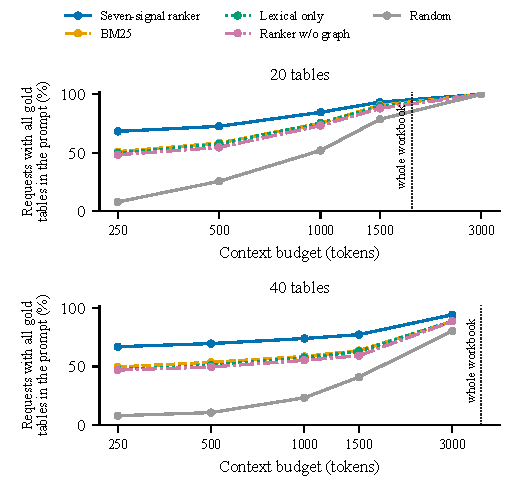
\includegraphics[width=\columnwidth]{figures/fig_e2_budget}
\caption{Share of requests whose prompt contains every gold table, by context budget, for workbooks with 20 and 40 tables. Dotted line: size of the whole workbook.}
\label{fig:e2}
\end{figure}

\begin{table}
\caption{Context retrieval on workbooks with 40 tables (300 requests). \emph{Complete}: share of requests whose prompt contains \emph{all} gold tables (\%); \emph{Recall}: mean fraction of gold tables retrieved (\%); \emph{Tokens}: mean prompt tokens spent on context.}
\label{tab:e2}

\centering\footnotesize
\begin{adjustbox}{max width=\columnwidth}\begin{tabular}{l rrr rrr}
\toprule
& \multicolumn{3}{c}{\textbf{Budget 1500}} & \multicolumn{3}{c}{\textbf{Budget 500}} \\
\cmidrule(lr){2-4}\cmidrule(lr){5-7}
\textbf{Method} & Complete & Recall & Tokens & Complete & Recall & Tokens \\
\midrule
Seven-signal ranker (shipped) & \textbf{77.3} & 77.3 & 1{,}488 & 69.7 & 69.7 & 487 \\
BM25 & 63.7 & 63.7 & 1{,}489 & 53.7 & 53.7 & 488 \\
Lexical (Jaccard) only & 63.0 & 63.0 & 1{,}488 & 51.0 & 51.0 & 487 \\
Ranker without graph signals & 59.3 & 59.3 & 1{,}488 & 49.7 & 49.7 & 488 \\
Ranker without lexical signal & 51.3 & 51.3 & 1{,}492 & 33.3 & 33.3 & 490 \\
Random & 41.0 & 41.0 & 1{,}487 & 10.7 & 10.7 & 490 \\
Active sheet only (as shipped to the agent) & 0.0 & 0.0 & 42 & 0.0 & 0.0 & 42 \\
Everything (no budget) & 100.0 & 100.0 & 3{,}723 & 100.0 & 100.0 & 3{,}723 \\
\bottomrule
\end{tabular}\end{adjustbox}
\end{table}


\paragraph{End-to-end study}
Table~\ref{tab:e5-taxonomy} gives the counts behind Figure~\ref{fig:e5-taxonomy}, and Table~\ref{tab:e5-repair-shipped} repeats the repair comparison with the chunk format the add-on shipped. Figure~\ref{fig:e5-templates} shows attempt-1 accuracy for every task template and model; the templates the local models fail are those that need a cross-sheet reference, a ranking or a conditional average. Table~\ref{tab:e5-cost} gives the generation cost.

\begin{table}
\caption{What verification sees among the formulas the model got wrong on its first attempt (final system). Flagged = rejected or warned.}
\label{tab:e5-taxonomy}

\centering\footnotesize
\begin{adjustbox}{max width=\columnwidth}\begin{tabular}{l rrrrrr}
\toprule
\textbf{Wrong at attempt 1} & \textbf{\shortstack[r]{Llama~3.1\\8B}} & \textbf{\shortstack[r]{Llama~3.2\\3B}} & \textbf{\shortstack[r]{Llama~3.1 8B\\new tasks}} & \textbf{\shortstack[r]{Gemini~3.1\\Flash-Lite}} & \textbf{\shortstack[r]{Gemini~3.5\\Flash-Lite}} & \textbf{\shortstack[r]{Gemma~4\\26B-A4B}} \\
\midrule
Wrong formulas & 105 & 220 & 50 & 8 & 12 & 15 \\
~~loud (engine error) & 67 & 110 & 29 & 1 & 3 & 4 \\
~~silent (wrong value) & 38 & 110 & 21 & 7 & 9 & 11 \\
Rejected by shipped verifier & 29 & 29 & 8 & 0 & 0 & 0 \\
Rejected by GroundCheck & 35 & 49 & 11 & 0 & 1 & 0 \\
Flagged by GroundCheck & 50 & 88 & 19 & 0 & 1 & 0 \\
Correct formulas rejected & 0/255 & 0/140 & 0/130 & 0/233 & 0/236 & 0/345 \\
\bottomrule
\end{tabular}\end{adjustbox}
\end{table}


\begin{table}
\caption{The repair comparison of Table~\ref{tab:e5-repair} repeated with retrieved context in the chunk format the add-on shipped (no column letters), forked from that arm's attempt 1.}
\label{tab:e5-repair-shipped}

\centering\footnotesize
\begin{adjustbox}{max width=\columnwidth}\begin{tabular}{l rr}
\toprule
& \multicolumn{2}{c}{\textbf{Llama~3.1 8B} (n=360)} \\
\textbf{Condition} & Acc. & $p_{\text{rs}}$ \\
\midrule
Attempt 1 & 64.4 & -- \\
Resample (no feedback) & 65.0 & -- \\
Generic feedback & 66.4 & .125 \\
Shipped-verifier feedback & 69.2 & <.001 \\
GroundCheck feedback & 70.3 & <.001 \\
GroundCheck + suspicious & 73.1 & <.001 \\
\bottomrule
\end{tabular}\end{adjustbox}
\end{table}


\begin{figure}[!t]
\centering
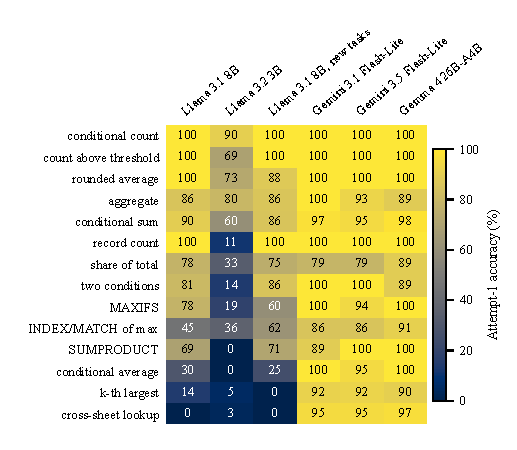
\includegraphics[width=\columnwidth]{figures/fig_e5_templates}
\caption{Attempt-1 accuracy with retrieved context by task template (rows) and model (columns); each cell is 11 to 58 tasks on the main set, 7 to 29 on the held-out set and at most 39 for each hosted model.}
\label{fig:e5-templates}
\end{figure}

\begin{table}
\caption{Generation cost per task by model: prompt tokens with the shipped active-sheet context and with retrieved context, wall-clock seconds for the first attempt (local models on one consumer GPU; hosted model over the network), and the extra model calls and seconds that repair with \gc{} feedback adds (--: not recorded in that pass).}
\label{tab:e5-cost}

\centering\footnotesize
\begin{adjustbox}{max width=\columnwidth}\begin{tabular}{l rrrrrr}
\toprule
\textbf{Per task} & \textbf{\shortstack[r]{Llama~3.1\\8B}} & \textbf{\shortstack[r]{Llama~3.2\\3B}} & \textbf{\shortstack[r]{Llama~3.1 8B\\new tasks}} & \textbf{\shortstack[r]{Gemini~3.1\\Flash-Lite}} & \textbf{\shortstack[r]{Gemini~3.5\\Flash-Lite}} & \textbf{\shortstack[r]{Gemma~4\\26B-A4B}} \\
\midrule
Prompt tokens, active sheet only & -- & 564 & 554 & 615 & 616 & 617 \\
Prompt tokens, retrieved context & 942 & 952 & 944 & 1{,}049 & 1{,}049 & 1{,}050 \\
Seconds, attempt 1 & 2.7 & 0.9 & 2.6 & 3.3 & 1.1 & 6.2 \\
Extra calls, \gc{} feedback & 0.13 & 0.21 & 0.10 & 0.00 & 0.00 & 0.00 \\
Extra seconds, \gc{} feedback & 0.4 & 0.2 & 0.3 & 0.0 & 0.0 & 0.0 \\
\bottomrule
\end{tabular}\end{adjustbox}
\end{table}


\section{Checking the labels in Google Sheets}
\label{app:gsheets}

The labels of \sheetfault{} come from HyperFormula, which follows Excel, while the system targets Google Sheets. To check that the labels carry over, the repository holds a validation harness: a stratified sample of \gsPackCases{} benchmark cases over \gsPackWorkbooks{} workbooks (\gsPackPerFault{} per fault class, \gsPackPerClean{} per clean class), an Apps Script that builds each case's workbook in a Google Sheet, puts the formula in the target cell and records what the cell shows, and a script that compares the two engines' answers case by case and re-derives the faulty/clean label under Google Sheets. The harness stops and resumes within the Apps Script time limit. Its control flow, resumption and comparison were tested against a mock of the Apps Script services backed by HyperFormula, on which all cases agree, as they must; that test says nothing about Google Sheets.

\ifdefined\gsN
Run in Google Sheets, the two engines give the same answer (an error in both, or the same value) for \gsSame\% of the \gsN{} cases: HyperFormula errs where Sheets does not in \gsHfErrOnly{}, Sheets errs where HyperFormula does not in \gsGsErrOnly{}, and the values differ in \gsDiffValues{}. The faulty/clean label is identical under both engines for \gsLabelSame\% of the cases (\gsFlipFault{} faulty under HyperFormula only, \gsFlipClean{} faulty under Sheets only). On the sampled faults \gc{} rejects \gsvtwoRecallHF\% under HyperFormula labels and \gsvtwoRecallGS\% under Google Sheets labels (shipped verifier: \gsvoneRecallHF\% and \gsvoneRecallGS\%), and rejects \gsvtwoFPRGS\% of the clean cases under Sheets labels.
\else
The run in Google Sheets is not part of this version of the paper, so every label here is a HyperFormula label. The harness reports the same quantities as the benchmark tables, so a run adds one paragraph to this appendix.
\fi

\section{Independent annotation of real formulas}
\label{app:annotation}

The real-formula sets have no labels (Section~\ref{sec:rwmethod}). The repository holds a protocol and tooling for blind annotation: a sample of 400 confirmation-set formulas stratified by the verifiers' decisions (\gc{} rejects, \gc{} only warns, only the shipped verifier rejects, both accept), shuffled and stripped of all verifier output, with the formula, its workbook's sheet names and sizes, the neighbourhood of the target cell and the sheets the formula names; written guidelines (defect Y/N/U, loud or silent, a category); a scorer that reports agreement between two annotators (raw and Cohen's $\kappa$), takes adjudicated labels for disagreements, and reports weighted precision, recall and false-positive rate of each verifier with workbook-clustered intervals. The tooling was tested on synthetic annotations only.

\ifdefined\annN
Two annotators labelled \annOf{} formulas independently; they agreed on \annAgree\% (Cohen's $\kappa$ \annKappa{}; \annKappaYN{} for defect against no defect) and settled \annDisagree{} disagreements together, leaving \annN{} formulas scored. Weighted back to the population, \annPrevalence\% of formulas are defective. On this ground truth the shipped verifier's rejections have precision \annVoneP\% [\annVonePLo, \annVonePHi] and recall \annVoneR\% [\annVoneRLo, \annVoneRHi]; \gc's have precision \annVtwoP\% [\annVtwoPLo, \annVtwoPHi] and recall \annVtwoR\% [\annVtwoRLo, \annVtwoRHi], with false-positive rates of \annVoneF\% and \annVtwoF\%.
\else
No annotation is part of this version: the numbers of Section~\ref{sec:e1b} are rejection rates, with an engine's evaluation as supporting evidence, and we claim no precision or recall on real formulas.
\fi


\end{document}
